%%%%%%%%%%%%%%%%%%%%%%%%%%%%%%%%%%%%%%%%%%%%%%%
%%																																	%%
%%  						Main file for my MSc Bioinformatics Dissertation										%%
%%																																	%%
%% 		Bioinformatics Analysis of a Phenol-Treated Acute Myeloid Leukaemia Cell Line 	%%
%% 																																	%%
%%%%%%%%%%%%%%%%%%%%%%%%%%%%%%%%%%%%%%%%%%%%%%%

%% Template used - https://github.com/jp-um/university_of_malta_LaTeX_dissertation_template

\RequirePackage[l2tabu, orthodox]{nag} % tells you of any bad LaTeX usage, must be first thing in class

%% There is one option you should define; oneside or twoside
%% Use twoside for your viva docs (examiners hate long docs they need to carry around)
%% and oneside for the final thing you submit to the library.  Note that margins will
%% change accordingly

\documentclass[twoside]{um}  % custom University of Malta project/dissertation/thesis 

%% **************** Packages start ******************

% \listfiles % uncomment this to know which packages you are using
              % the list of packages will be in the bottom of the .log file
\usepackage{booktabs}
\usepackage{listings}
\usepackage{xcolor}
\usepackage{hyperref}
\usepackage{float}
\usepackage{array}
\usepackage{changepage}
\usepackage{caption}

%New colors defined below
\definecolor{codegreen}{rgb}{0,0.6,0}
\definecolor{codegray}{rgb}{0.5,0.5,0.5}
\definecolor{codepurple}{rgb}{0.58,0,0.82}
\definecolor{backcolour}{rgb}{0.95,0.95,0.92}

% Sets list line spacing
\usepackage{enumitem}
\setlist[enumerate]{itemsep=0mm}

%Code listing style named "mystyle"
\lstdefinestyle{mystyle}{
		language=bash,
		backgroundcolor=\color{backcolour}, 
		commentstyle=\color{codegreen},
		keywordstyle=\color{magenta},
		stringstyle=\color{codepurple},
		numberstyle=\tiny\color{codegray},
		basicstyle=\ttfamily\footnotesize,
		captionpos=b,                    
		keepspaces=true,                 
		numbers=left,                    
		numbersep=5pt,                  
		showspaces=false,                
		showstringspaces=false,
		showtabs=false,                  
		tabsize=1
}

\lstset{style=mystyle}

\newcommand{\mkbibnodate}{n\adddot d\adddot}


%% Note that packges may already be loaded from the um (and memoir) classes.
%% Do not add your packages to the template, but rather add them here.

%% ***************** Packages end *******************

%% **************** (Your) Data (Start) ******************

\title{RNA-seq Analysis of an \\ Acute Myeloid Leukaemia \\ Cell Line Treated with \\ Phenolic Compounds}  % use \\ here otherwise you get a justified title
                                     % note capitalization of the title (only common words in lower case)
%\tagline{Do I need this here?}
\author{Matthew Pace} 
\authorID{372098M}
\supervisor{Dr Lucienne Vassallo Gatt}
\cosupervisor{Dr Jean-Paul Ebejer\\and Dr Marion Zammit Mangion }           
\department{Centre for Molecular Medicine & Biobanking}   
\faculty{Faculty of Health Sciences}       
\degreeName{M.Sc.\ in Bioinformatics}       % note the \ after the dot, so not to consider it a fullstop
\doctype{dissertation}
\degreeDate{\monthyeardate\today}    % when did you submit (officially after your corrections)
%\subjectcode{MMB5010}                % currently not used

%% ***************** (Your) Data (End) *******************


%% ******** (Your) Document Settings (Start) *************

% You should have an images directory in every chapX subdir
% NOTE:  Trailing / for subdirs is required.
\graphicspath{{./images/}{./intro/images/}{./lit_review/images/}{./method/images/}{./conclusion/images/}{./evaluation/images/}{./results/images/}}   
% Paths where to look for images, if defined "images" must always be there as it holds the images in-use by the template.

\makeindex

%% ********* (Your) Document Settings (End) **************

% DOCTOR'S (JP) ORDERS: MAKE SURE TO READ MY TWO BLOG ENTRIES WITH
% CONTENT AND LaTeX TIPS FOR YOUR WRITE-UP.  THESE ARE BASED ON  
% EXAMINER'S FEEDBACK
%
% URLS:
% https://bitsilla.com/blog/2019/03/content-tips-for-your-dissertation-or-project-write-up/
% https://bitsilla.com/blog/2019/01/latex-tips-for-your-dissertation-or-project-write-up/

% end the preamble and start the document

\begin{document}
\frontmatter 
    % \maketitle
    % \begin{copyrightenv}
\end{copyrightenv}
       
    % \begin{originality}
\end{originality}    
    % \begin{dedication}
{\large{To The Avengers}}\\[5mm]
You know, for saving the world.
\end{dedication}

        % include a dedication.tex file
    % \begin{acknowledgements}
\textbf{These are the acknowledgements.}
\end{acknowledgements}   % include an acknowledgements.tex file
     % %% For tips on how to write a great abstract, have a look at
%%	-	https://www.cdc.gov/stdconference/2018/How-to-Write-an-Abstract_v4.pdf (presentation, start here)
%%	-	https://users.ece.cmu.edu/~koopman/essays/abstract.html
%%	-	https://search.proquest.com/docview/1417403858
%%  - 	https://www.sciencedirect.com/science/article/pii/S037837821830402X

\begin{abstract}
\textbf{This is the abstract.} 
It is hard to overstate the revolutionary changes brought about by Next-generation sequencing to the realm of biomedical research.


\end{abstract}\if@openright\cleardoublepage\else\clearpage\fi
    \tableofcontents*\if@openright\cleardoublepage\else\clearpage\fi
    \listoffigures*\if@openright\cleardoublepage\else\clearpage\fi
    %\listoftables*\if@openright\cleardoublepage\else\clearpage\fi
    \chapter*{List of Abbreviations}
% Fix spacing

\markboth{List of Abbreviations}{List of Abbreviations}
               
\begin{acronym}\itemsep-20pt\parsep-20pt %% if you remove these spacing params this list becomes huge!
\acro{AML}{Acute Myeloid Leukaemia}
\acro{QC}{Quality Control}
\acro{ATRA}{all-\textit{trans} retinoic acid}
\acro{TMM}{Trimmed Mean of \textit{M}-values}
\acro{RIN}{RNA Integrity Number}
\acro{PCR}{Polymerase Chain Reaction}
\acro{FAB}{French-American-British}
\acro{WHO}{World Health Organisation}
\acro{EMBL}{European Molecular Biology Laboratory}
\acro{HPLC}{High-Performance Liquid Chromatography}
\acro{HSC}{Hematopoietic Stem Cells}
\acro{LLE}{Liquid-Liquid Extraction}  
\acro{STAR}{Spliced Transcripts Alignment to a Reference}
\acro{NGS}{Next-Generation Sequencing}
\acro{TPM}{Transcripts Per Million}
\acro{SNP}{Single Nucleotide Polymorphism}
\acro{DEG}{Differentially Expressed Genes}
\acro{DGE}{Differential Gene Expression}
\acro{BCV}{Biological Coefficient of Variance}
\acro{MMP}{Maximum Mappable Prefix}
\acro{FDR}{False Discovery Rate}
\acro{GO}{Gene Ontology}
\acro{KEGG}{Kyoto Encyclopedia of Genes and Genomes}
\acro{GSEA}{Gene Set Enrichment Analysis}
 
\end{acronym}

\iffalse
\usepackage{glossaries}

\makeglossaries
               
\newglossaryentry{AML}{name=AML, description={Acute Myeloid Leukaemia}}
\newglossaryentry{QC}{name=QC, description={Quality Control}}
\newglossaryentry{ATRA}{name=ATRA, description={all-\textit{trans} retinoic acid}}
\newglossaryentry{TMM}{name=TMM, description={Trimmed Mean of \textit{M}-values}}
\newglossaryentry{FAB}{name=FAB, description={French-American-British}}
\newglossaryentry{WHO}{name=WHO, description={World Health Organisation}}
\newglossaryentry{EMBL}{name=EMBL, description={European Molecular Biology Laboratory}}
\newglossaryentry{HPLC}{name=HPLC, description={High-Performance Liquid Chromatography}}
\newglossaryentry{HSC}{name=HSC, description={Hematopoietic Stem Cells}}
\newglossaryentry{LLE}{name=LLE, description={Liquid-Liquid Extraction}}
\newglossaryentry{STAR}{name=STAR, description={Spliced Transcripts Alignment to a Reference}}
\newglossaryentry{NGS}{name=NGS, description={Next-Generation Sequencing}}
 \newglossaryentry{TPM}{name=TPM, description={Transcripts Per Million}}
 \newglossaryentry{SNP}{name=SNP, description={Single Nucleotide Polymorphism}}
 \newglossaryentry{DEG}{name=DEG, description={Differentially Expressed Genes}}
\newglossaryentry{DGE}{name=DGE, description={Differential Gene Expression}}
 \newglossaryentry{BCV}{name=BCV, description={Biological Coefficient of Variance}}
 \newglossaryentry{FDR}{name=FDR, description={False Discovery Rate}}
 \newglossaryentry{GO}{name=GO, description={Gene Ontology}}
\newglossaryentry{KEGG}{name=KEGG, description={Kyoto Encyclopedia of Genes and Genomes}}
 
\printglossaries
\fi\if@openright\cleardoublepage\else\clearpage\fi
    %\lstlistoflistings

%% Note: always use \input as you cannot nest \includes (amongst other things)
\pagestyle{umpage}
\floatpagestyle{umpage}
\mainmatter 
    \chapter{Introduction}
\label{intro}
Leukaemia is a cancer of the hematopoietic system, and is classified according to the affected cell lineage and according to its rate of development, thus \textit{acute myeloid leukaemia} refers to a particularly aggressive and rapidly proliferating class of leukaemia which affects the myeloid cell line. This occurs when undifferentiated myeloid cells called myeloblasts acquire mutations which hinder further differentiation but allow for their rapid clonal proliferation \citep{Khwaja2016}. The causative genetic or cytogenetic abnormalities which induce cancer are expressed in the cell's transcriptome, which can be quantified into discrete transcripts using RNA sequencing (RNA-seq). 

RNA-seq is the application of \ac{NGS} techniques to measure the quantity of RNA sequences in a biological sample, in a given moment \citep{zhong2009}. It has gradually replaced microarrays as the standard method of measuring a cell's RNA profile, offering less technical noise, high throughput of transcriptomic data, and a lower overall cost for the mapping of large transcriptomes \citep{zhao2014comparison, rao2019comparison}. 

In this dissertation we will use this technology to detect whether a phenolic treatment was successful in inducing differentiation in HL-60 cells, an \ac{AML} cell-line. If differentiation can be induced in \ac{AML}, the undifferentiated myeloid cells will be forced to take an epigenetic path (e.g. towards becoming a monocyte), culminating in apoptosis \citep{santos2000expression, mark2017transcriptomes}. This fundamental transformation of the cells is reflected in their transcriptome. A 'snapshot' of the cell's transcriptomes will be taken at three time-points (1hr, 6hr, 12hr) after the administration of the treatment, which will be compared to the transcriptome of a fourth sample, the negative control (which may be regarded as the time-point '0hr') through differential gene expression analysis. If the treatment was successful, we should expect to see differential expression in genes involved in pathways related to apoptosis, cancer and differentiation.



\section{Motivation} 
Despite incremental improvements in treatment over the past few decades, average \ac{AML} 5-year survival rates remain at 28\% for affected individuals, which decreases with age and unfavourable cytogenetics, according to the SEER database \citep{sasaki2021novo}. Chemotherapy is currently standard practice for the treatment of \ac{AML}, despite its indiscriminate cytotoxic effects and resultant physiological consequences on the patient. As a result of their frail state, older adults usually cannot withstand the side-effects of this treatment and are instead put under palliative care with abysmal chances of even short-term survival \citep{lancet2018overall}. 

Recent decades have seen rapid progress in high-throughput sequencing techniques and our understanding of cancer biology, which have lead to the development of novel targeted treatments. One of these relatively recent approaches is differentiation therapy, where a pharmacological agent encourages differentiation in cancer cells. This alters the cancer's immature, stem-cell like state, halting its ability to rapidly proliferate and metastasise. The differentiation agent \ac{ATRA} has been particularly successful in treating the \ac{AML} subtype of acute promyelocytic leukaemia (APL), managing to achieve a 90\% survival rate, while avoiding the severe cytotoxic side-effects of chemotherapy \citep{kim2015selection}. This dissertation is an attempt to use recent developments in RNA-seq technology to potentially identify a similarly acting compound to further increase our arsenal in our war against cancer, specifically against \ac{ATRA}-resistant strains of \ac{AML}, whilst sparing the patient of the severe side-effects associated with chemotherapy.


\section{An Introduction to RNA-seq}

The specifics of the RNA-seq workflow are highly variable, with many competing techniques for many steps in the process currently in use. A generic representation of the wet-lab processes involved can be seen in Figure \ref{fig:rnaseq_biorender}. An essential step common to every workflow is the extraction of RNA from the sample tissue or cells. This is a particularly tricky endeavour as RNA is chemically unstable due to the hydroxyl groups at the 2' and 3' positions, facilitating RNase activity (RNA-degrading enzymes) \citep{green2019win}. This issue is compounded by the ubiquity and chemical resilience of RNAses, meaning that special care must be taken to avoid contamination of glassware and instruments that interact with the RNA \citep{green2019win}. The sample is lysed to extrude the contents of the cell, and DNA and proteins are removed via phase separation between two immiscible liquids. The end result should be the high-quality RNA in an aqueous solution. The resulting RNA is composed of messenger RNA (mRNA), transfer RNA (tRNA) and various other categories of non-coding RNA (ncRNA), most notably ribosomal RNA which makes up 95\% of the total RNA and is irrelevant to our analysis \citep{kukurba2015rna}. This bulky rRNA is removed using oligo-dT primer beads or commercially available kits specific to the removal of rRNA \citep{peano2013efficient}. The next chronological step is library preparation, where RNA strands are fragmented, converted to their complimentary DNA (cDNA) strands and ligated to adapter sequences \citep{zhong2011high}. This adapter-ligated cDNA library is typically attached to a flow-cell, amplified and sequenced in a high-throughput sequencing platform which typically results in a FASTQ \citep{cock2010sanger} file. % Include more detail here?
This contains the nucleotide sequence of the cDNA in a text-based format. Each nucleotide base call is also assigned an ASCII character as a quality score. Phred quality scores are among the most widely used, which are numerical scores generally ranging from 10 to 60, logarithmically related to the probability of an erroneous base-call, represented as a single ASCII character \citep{ewing1998base}.

\begin{figure}[ht!]
  \centering
  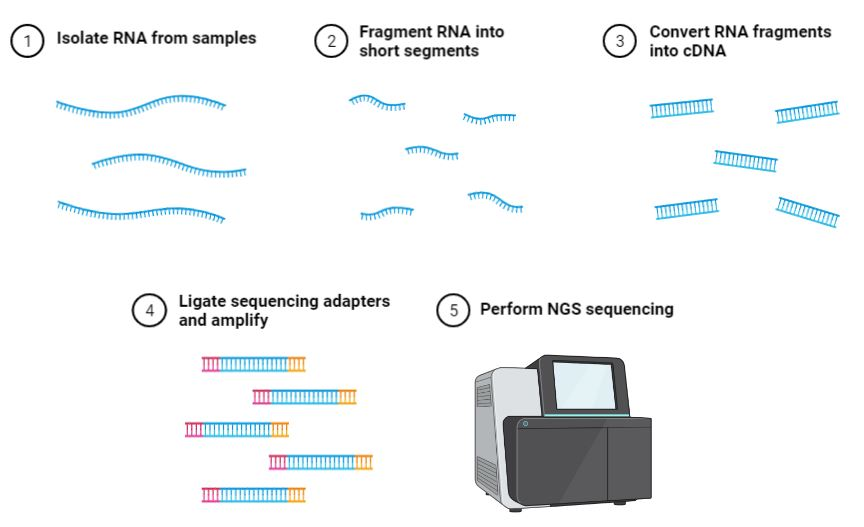
\includegraphics[width=0.9\linewidth]{rnaseq_biorender}
  \caption[Summary of the wet-lab processes which occur prior to RNA-seq data analysis.]{Summary of the wet-lab processes which occur prior to RNA-seq data analysis. Created using \href{https://biorender.com/}{BioRender.com}.}
  \label{fig:rnaseq_biorender}
\end{figure}

This brings us to the part of RNA-seq which was performed during this dissertation: the data analysis. This involves the construction of a pipeline consisting of multiple tools stitched together with the aim of gaining insight on the differentially expressed genes between samples. As a result of the decentralised nature of bioinformatics, and the potential variability of the data and goals of the researcher, there is no one-size-fits-all tool. The researcher constructing the pipeline must take into account a myriad of trade-offs for each tool for each step of the pipeline. However the steps to an RNA-seq pipeline protocol can be generalised as:
\begin{enumerate}
\item \textbf{Quality Control} - This involves the visualisation of the sequencing data to assess its quality, identifying any potential sequencing errors. This step translates the quality scores embedded in FASTQ files into something more interpretable such as a line graph. Other common quality metrics may include GC content, the number of \textit{N} symbols and presence of adapter sequences. Recognising certain patterns in data quality visualisation is essential to identifying the source of the problem \citep{stoler2021sequencing}.
\item \textbf{Preprocessing} - This is an optional step performed only if \ac{QC} indicates that there are issues with the data. Adapter sequences, low-complexity regions and low Phred scores are considered \textit{low-quality}, thus have a high probability of being erroneous and are discarded \citep{martin2011cutadapt, prinseq++}. Other metrics (e.g. GC content) are harder to amend, and may be indicative of a deeper problem further upstream in the process. 
\item \textbf{Alignment} - Reads are compared to a reference genome or reference transcriptome and aligned to the regions of highest similarity. Aligners typically first find an exact match between the two, which they use as a \textit{seed}. The seed is extended through an implementation of dynamic programming to find the optimal alignment.
\item \textbf{Quantification} - This step produces a gene count matrix containing the number of reads which fall within the coordinates of a particular gene. Typically, the row names would be gene IDs and column names would be the sample IDs, with each cell representing the number of reads which fall within that gene region.
\item \textbf{Normalisation} - Confounding variables which are not biologically relevant and induce differences between samples and between genes must be accounted for for an unbiased comparison of samples. The main factors to account for are sequencing depth \citep{robinson2010scaling}, gene length \citep{oshlack2009transcript} and GC content \citep{risso2011gc}. This step may be fused with the previous or following one depending on the tool. 
\item \textbf{Differential Expression} - Statistical tests are performed to see whether a significant difference exists between the normalised sample read counts and a benchmark sample considered to be 'normal' or 'healthy'. Every compared gene typically produces two values: the $log_{2}$ fold-change (logFC) and the p-value (adjusted for multiple testing). A threshold is applied to each of these to determine which genes should be considered as differentially expressed. If the logFC is positive, the gene is up-regulated, while if it is negative, the gene is considered down-regulated when compared to the benchmark sample.
\item \textbf{Downstream analysis} - Typically involves some form of visualisation of the \ac{DEG} to gain biological insight, but further analysis depends greatly on the research question. Possible routes are gene expression clustering, pathway analysis and functional term over-representation analysis \citep{conesa2016survey, chung2021best}.
\end{enumerate}

\section{Aim and Objectives} 
\label{Aim and Objectives}
This dissertation shall be performing RNA-seq analysis on data generated during a PhD thesis by \cite{Gatt2016}. During this preliminary study, an \ac{ATRA}-resistant HL-60 cell line was used to model \ac{AML}, and was treated with a phenolic mixture across four time-points (further detail in the Section \ref{method:prelim study}). The general aim of this dissertation is to provide insight into the molecular mechanism of differentiation caused by the phenol treatment on the \ac{ATRA}-resistant HL-60 cells over time through bulk RNA-seq analysis. To achieve this, six objectives must be attained:

\begin{enumerate}
\item Determine which bioinformatics tools are best suited to be used in this RNA-seq pipeline given the current data
\item Perform quality control checks on the data files at various stages of analysis to identify and adjust poor quality data
\item Assign genes to each read through the alignment to a recent human reference genome or transcriptome release
\item Conduct differential expression analysis between the treated samples and the untreated control
\item Annotate, visualise and interpret the gene expression data in its biological context to provide insight into which gene-sets are being affected by the phenol treatment over time
\end{enumerate}


%\begin{figure}[ht!] % supposedly places it here ...
%  \centering
%  
\includegraphics[width=0.6\linewidth]{test_image_goku}
%  \caption[This is the short caption for List of Figures]{A test figure.  This caption is huge, but in the list of figures only the smaller version in the square brackets will appear.\index{Goku il-king}}
%  \label{fig:test1}
%\end{figure}
%A test figure is shown in Figure~\ref{fig:test1}.

%\begin{figure}[!ht]
%    \centering
%    \subbottom[Goku]{
\includegraphics[width=0.3\textwidth]{test_image_goku}}\qquad
%    \subbottom[More Goku]{
\includegraphics[width=0.3\textwidth]{test_image_goku}}%
%    \caption[Short Caption]{The same super saiyan. Two times.} 
%  \label{fig:test2}
%\end{figure}

%Two figures shown side by side are shown in Figure~\ref{fig:test2}.

\section{Our Approach}
The first step to achieve the stipulated aim was a thorough literature review to become acquainted with commonly used tools in RNA-seq analysis and their respective limitations and trade-offs. This allowed for the identification of the optimal tools suited for our dataset, which can be described as a time series with four time points, with a single sample per time point.

FastQC is an essential starting point in any Omic data analysis, due to its provision of extensive quality metrics. FastQScreen \citep{wingett2018fastq} added another layer of information by checking the sequences against multiple reference genomes, human and non-human, to check for contamination. Cutadapt \citep{martin2011cutadapt} was used to trim adapter sequences and short reads. Prinseq++ \citep{prinseq++} was then used to remove ambiguous reads and regions of low-complexity. The trimmed and filtered FASTQ files were aligned to the GRCh38.p13 reference genome \citep{ref} using the \ac{STAR} aligner \citep{Dobin2013}. \ac{STAR} was called through RSEM \citep{li2011rsem}, which after alignment, estimates gene and isoform expression levels. 

The four gene count files, containing the gene IDs and expected read counts, were imported into R \citep{R} to follow the edgeR \citep{edger} workflow, including \ac{TMM} normalisation. A negative control sample (which may be referred to as the '0 hour' time point) was used as the baseline to which the three other time points where compared to in a pairwise comparison fashion. Due to budget constraints, there were a lack of replicates in this study. While a common and often unavoidable consequence of the high costs associated with RNA-seq experiments, severely restricted the possible options for differential expression analysis. The statistical tests used by the leading \ac{DGE} tools edgeR and DESeq2 \citep{love2014moderated} both require the estimation of dispersion, which cannot be calculated using a single sample. As a workaround, the edgeR vignette\footnote{https://www.bioconductor.org/packages/release/bioc/vignettes/edgeR/inst/doc/edgeRUsersGuide.pdf} suggests an approximated value for the Biological Coefficient of Variation (BCV) based on similar studies, from which we can derive the dispersion. This approach, although inaccurate, was deemed as the most suitable method of \ac{DGE} given this dataset. These \ac{DEG}s were annotated and visualised for an overview of the differences between the samples, particularly how the transcriptome of the untreated samples changed over time with treatment. Pathway analysis was performed with a particular focus on those infamously deranged by cancer to gain further biological insight on the differentiation process occurring.

% Revisit this part later

\section{Document Structure}
This chapter has provided a surface-level introduction to the theory behind this project, why it was undertaken and what it hopes to achieve.

In the following chapter, the \textbf{Background and Literature Overview} we will delve deeper into what is currently known about \ac{AML} and RNA sequencing techniques. It will provide an overview of the relevant literature, in particular recent studies which made use of RNA-seq analysis pipelines, and how their methods and findings influenced this project.

\textbf{Methodology} will focus on the work done to achieve the aforementioned aim and objectives. We will summarise the preliminary wet-lab work performed by Dr Vassallo Gatt  \citep{Gatt2016}, and describe in detail the steps taken to construct the RNA-seq pipeline to transform the data in four FASTQ files.

In the \textbf{Results \& Discussion}, we will present the outputs of the steps described in the previous chapter, followed by a detailed interpretation. will describe the reasoning behind the construction of the RNA-seq pipeline, and justify the choice of tools and their chosen parameters. It will also compare and contrast our results with the results of previous literature, particularly the top \ac{DEG}s and deranged pathways found in this study, with those associated with \ac{AML}. 

The final chapter, the \textbf{Conclusion}, will revisit the aim and objectives and discuss if there were achieved to a satisfactory degree. Here we will give a final summary of our interpretation of the results, what could have been improved, and proposals for future work on the topic.

 
    \chapter{Background \& Literature Overview}
\label{lit review}

The typical multicellular organism stores its genetic code as deoxyribonucleic acid (DNA), found identically in all its somatic cells (unless \textit{de novo} mutations occur). DNA is a biological polymer, consisting of a double-stranded polynucleotide chain. Each nucleotide monomer consists of a phosphate group, deoxyribose (a five-carbon sugar), and one of four nucleobases: adenine (A), cytosine (C), guanine (G), or thymine (T). These two strands are held together with a series of hydrogen bonds between the nucleobases, forming Watson-Crick base pairs. %On opposite strands, adenine and thymine form double hydrogen bonds, while guanine and cytosine form a stronger triple hydrogen bond.

DNA is just the general starting point in a series of information transfers described by the \textit{Central Dogma of Molecular Biology}, which the cell uses to ultimately produce its molecular products \citep{cobb201760}. Through the process of \textit{transcription}, the code from one strand of DNA is transferred onto a primary ribonucleic acid (RNA) transcript. RNA is similar to DNA except that it is single-stranded, has ribose as its five-carbon sugar and uses the nucleobase \textit{uracil} instead of \textit{thymine}. This primary transcript is modified into ribosomal RNA (rRNA), transfer RNA (tRNA) or messenger RNA (mRNA). All three are involved in \textit{protein synthesis}, although mRNA is especially relevant to this project since the protein sequence can be deduced from the mRNA sequence. These molecular products shape the cell's appearance, define how it interacts with external or internal stimuli, and allows it to perform its intended functions. They give each cell type a characteristic RNA profile which can be measured through RNA-seq. Using this technology, we can detect the presence or absence of certain transcriptomic hallmarks of cancer.

% the intro for this is pretty good: https://www.nature.com/articles/s41368-021-00146-0#:~:text=Bulk%20RNA-seq%20studies%20average%20global,next%20generation%20of%20RNA%20sequencing.

%\clearpage
%\section{Differentiation Pathways in the Haematopoietic System}
%. Acute leukaemia occurs earlier in the differentiation pathway, allowing the blasts to divide more rapidly. \autoref{fig:cell_differentiation} shows the mature cell types that result from myeloid and lymphoid cell lineages, which both share \ac{HSC} as the common progenitor cell type.

\clearpage
\section{Acute Myeloid Leukaemia}

%good resource: https://btep.ccr.cancer.gov/wp-content/uploads/RNA-seq_BETP_2019rev.pdf

\ac{AML} is an aggressive form of cancer of the haematopoietic system (\autoref{fig:cell_differentiation}) which is characterised by its rapid proliferation of myeloblasts. This occurs when undifferentiated myeloid cells acquire mutations which hinder further differentiation but allows for their clonal proliferation \citep{Khwaja2016}. This comes at the expense of the production of their healthy, differentiated counterparts: erythrocytes, platelets and granulocytes \citep{Khwaja2016}. It is an exception to cancers in that it does not form a tumour, which is usually analysed to determine the severity. Instead \ac{AML} is staged according to its subtype and other variables \citep{ACS2018}. It is the most common form of acute leukaemia, with an incidence rate of 4.3 per 100,000 in the United States \citep{Kouchkovsky2016}. One of the main risk factors is age, with a median age of diagnosis of 70 years, and with a slight male predominance \citep{juliusson2009age, Khwaja2016}. Acute myeloid leukaemia is synonymous with acute myelogenous leukemia, acute myelocytic leukemia, or acute nonlymphocytic leukemia.

%Summary of leukaemia: https://www.cancer.net/cancer-types/leukemia-acute-myeloid-aml/introduction

\begin{figure}[!h]
    \centering
    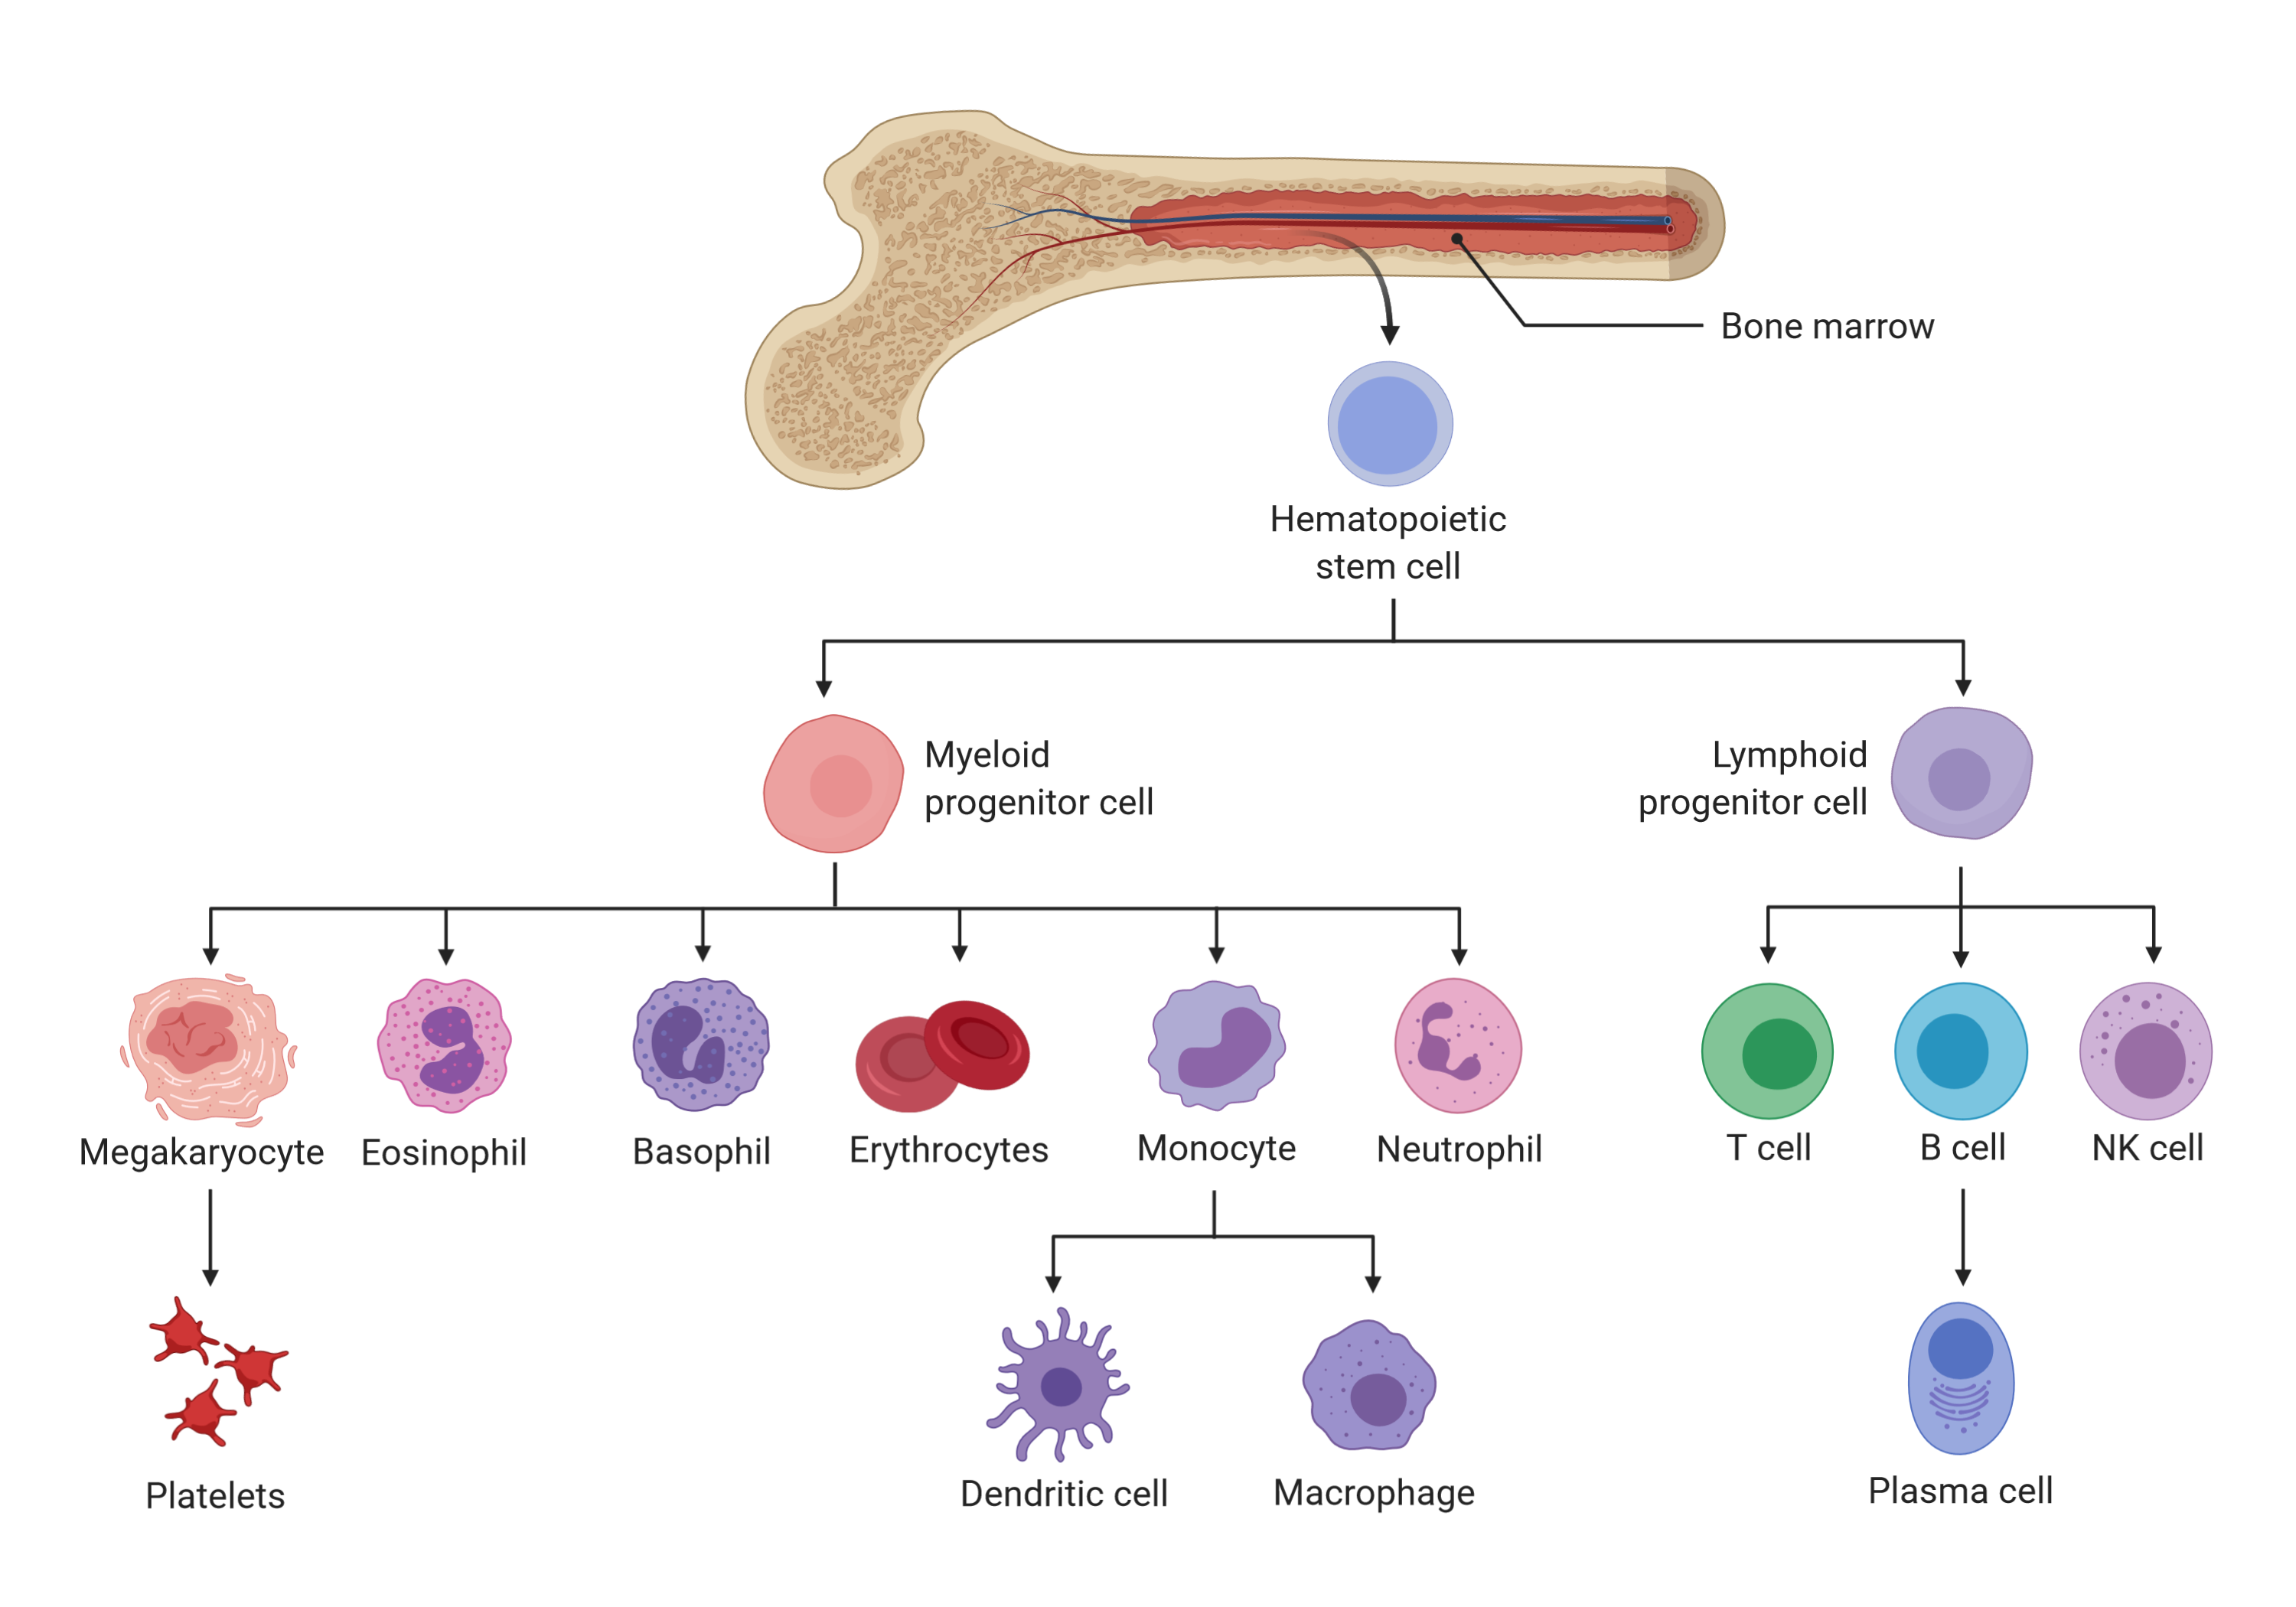
\includegraphics[width=1\textwidth]{cell_differentiation}
    \caption[Stem cell differentiation]{An overview of the main branches of haematopoietic stem cell differentiation pathways showing the myeloid and lymphoid lineages. Created using \href{https://biorender.com/}{BioRender.com}. } 
    \label{fig:cell_differentiation}
\end{figure}

\subsection{Classification and Subtypes}
\label{Classification and Subtypes}
\ac{AML} is one of four main branches of leukaemia classification, the others being Acute Lymphoblastic Leukaemia (ALL), Chronic Myeloid Leukaemia (CML) and Chronic Lymphoblastic Leukaemia (CLL) \citep{leukaemiabook}. Despite their cytogenic differences, there have been multiple reports of chronic leukaemia types transitioning into the more aggressive, acute form over time \citep{kaur2016rapid, frenkel1981acute, jacobs1984acute}. Treatment may vary depending on the subtype of the disease, which is why a rigid classification system and correct identification is important \citep{leukaemiabook}.

Each of these four leukaemia subtypes is subdivided into more specific classifications. \ac{AML} in particular is genetically and morphologically heterogeneous and can involve any single or a combination of myeloid lineages \citep{whoclassification, Kouchkovsky2016}. 

\subsubsection{The FAB classification system}
The \ac{FAB} classification, first produced in 1976, was an early attempt to distinguish subtypes of \ac{AML} \citep{bennett1976proposals}. The divisions were based on cell morphology and the relative quantities of myeloblasts and erythroblasts \citep{ACS2018}.

%Maybe lookup cool table latex tutorials to make it nicer (colours maybe?)
\begin{table}[h]
\centering
\caption{The FAB classification of AML.}
\label{tab:FABclassification}
\begin{tabular}{lll}
\hline
M0 & Undifferentiated acute myeloblastic leukemia        &  \\ 
M1 & Acute myeloblastic leukemia with minimal maturation &  \\
M2 & Acute myeloblastic leukemia with maturation         &  \\
M3 & Acute promyelocytic leukemia (APL)                  &  \\
M4 & Acute myelomonocytic leukemia                       &  \\
M5 & Acute monocytic leukemia                            &  \\
M6 & Acute erythroid leukemia                            &  \\
M7 & Acute megakaryoblastic leukemia                     &  \\ \hline
\end{tabular}
\end{table}

% AML categories are extremely heterogeneous, probably due to high genetic diversity

\subsubsection{The WHO classification system}

A more modern, and now more widely used system, is that devised in the \textit{\ac{WHO} Classification of Tumors of Hematopoietic and Lymphoid Tissues}, now in its revised 4th edition \citep{whoclassification}. \ac{AML} is here defined as having >20\% of the cells in the bone marrow being myeloblasts. The \ac{WHO} based their classification on a mixture of genetic, morphological and cytochemical criteria and based on the presence of other conditions. They define seven subcategories:

\begin{enumerate} \itemsep-0.5em
\item AML with recurrent genetic abnormalities
\item AML with myelodysplasia-related changes (MRC)
\item Therapy-related myeloid neoplasms (t-MN)
\item AML related to previous chemotherapy or radiation
\item Myeloid sarcoma (also known as granulocytic sarcoma or chloroma)
\item Myeloid proliferations related to down syndrome (DS)
\item AML with chromosomal translocations and inversions
\end{enumerate}

These may be further classified according to their specific genetic or karyotypic abnormalities \citep{whoclassification}. Cases which do not fall into any of the above groups, are labelled as 'AML, not otherwise specified (NOS)' and are subject to a form of classification similar to the \ac{FAB} \citep{ACS2018}. Cases classified as having 'recurrent genetic abnormalities' are often sub-categorised and described according their their abnormality (similar to Table \ref{tab:karyotype}, although not all are officially recognised as 'recurring abnormalities').

%https://emedicine.medscape.com/article/2006750-overview?reg=1
%https://www.ncbi.nlm.nih.gov/books/NBK560490/

\subsection{Pathogenesis}
\label{Pathogenesis}
The genetic abnormalities leading to \ac{AML} are heterogeneous and complex, meaning that there are many different combinations of causative genetic or cytogenetic abnormalities which may lead to the \ac{AML} phenotype \citep{lindsley2015acute, whoclassification}. The genetic and karyotypic profile can have profound prognostic impact, affecting both therapeutic strategy and survival rate \citep{mrozek2000prognostic, whoclassification}. 

\subsubsection{Cytogenic Abnormalities}
Approximately 55\% of \ac{AML} patients have at least one cytogenic abnormality \citep{meyer2014translational}.  \cite{stolzel2016karyotype} note that patients with 3 unrelated cytogenic abnormalities, have a worse overall survival rate than \ac{AML} patients with a normal karyotype, and that the patients at most risk had $ \geq $4 unrelated cytogenic abnormalities. There are some exceptions, where the presence of certain abnormalities actually \textit{increases} survival rate with good response to treatment (Table \ref{tab:karyotype}). 

\begin{landscape}
	\pagestyle{empty} % to remove headers on the side	
\begin{table}[h]

    \centering
    \caption{Recurrent abnormalities in AML and their effects. This table makes use of the International System for Human Cytogenomic Nomenclature (ISCN) to describe chromosomal abnormalities \citep{ISCN}. The information given prior to the parentheses denotes the type of chromosomal abnormality (for example \textit{t} for translocation, and \textit{inv} for inversion). The contents of the first pair of parenthesis refer to the affected chromosome(s). The second pair of parentheses, if present, refers to the specific part of the respective chromosome(s) affected (the short arm \textit{p} or the long arm \textit{q}, and which region or band of these arms).}
    \label{tab:karyotype}
    \begin{tabular}{lllllllllllll}
    \toprule
        \textbf{Aberration} & \textbf{Prognosis} & \textbf{Fusion Genes} & \textbf{Note} & \textbf{Reference}  & ~ \\ \midrule
        t(8;21)(q22;q22) & Favourable & RUNX1, RUNX1T1 & Common (\textasciitilde 5\% of all AML) & \cite{reikvam2011acute}  & ~ \\ 
        ~ & ~ & ~ & ~ & \cite{peterson20048}  & ~ \\ \hline
        inv(16)(p13;q22) & Favourable & CBFB, MHY11 & Common & \cite{plantier1994inv}  & ~ \\ 
        t(16;16)(p13;q22) & ~ & ~ & ~ & \cite{shigesada2004mechanism}  & ~ \\ \hline
        t(15;17)(q24;q21) & Favourable & PML, RARA  & Common (\textasciitilde 10\% of adult AML) & \cite{de2014rara}  & ~ \\ 
        ~ & ~ & ~ & ~ &   & ~ \\ \hline
        t(9;11)(p22;q23) & Poor & KMT2A, MLLT3 & Frequency decreases with age & \cite{chandra2010acute}  & ~ \\ 
        ~ & ~ & ~ & ~ & \cite{metzler2004emergence}  & ~ \\ \hline
        t(6;9)(p23;q34) & Poor & DEK, CAN/NUP214 & Rare, associated with an internal tandem & \cite{chi2008acute}  & ~ \\ 
        ~ & ~ & ~ &  duplication (ITD) mutation on FLT3 &   & ~ \\ \hline
        inv(3)(q21.3;q26.2) & Poor & RPN1, MECOM & Rare, low response to standard  & \cite{sitges2020acute} & ~ \\ 
        t(3;3)(q21.3;q26.2) & ~ & ~ & chemotherapy & ~ & ~ \\ \hline
        t(1;22) (p13;q13) & Poor & RBM15, MKL1 & Rare, almost exclusively found in infants   & \cite{carroll1991t} & ~ \\ 
        ~ & ~ & ~ &  with acute megakaryocytic leukaemia & \cite{bernstein2000nineteen} & ~ \\ \hline
        Monosomy  & Very poor & / & Loss of chromosome, frequency increases & \cite{breems2008monosomal} & ~ \\ 
        ~ & ~ & ~ &  with age &   & ~ \\ \bottomrule
    \end{tabular}
\end{table}
\end{landscape}


%t(8;21) is a frequently oc­curring aberration in acute AML. It involves the fusion of the RUNX1 (runt-related transcription factor 1) gene on chromosome 21q22 and the RUNX1T1 (runt-related transcription factor 1; translocated to 1) gene on chromosome 8q22, resulting in the formation of the hybrid gene RUNX1/RUNX1T1. AML with t(8;21)(q22;q22), RUNX1/RUNX1T1 generally shows maturation in the myeloid lineage and is found in approximately 5\% of cases of AML. cite:https://atlasgeneticsoncology.org/haematological/1019/t(8;21)(q22;q22)-runx1-runx1t1

% SUMMARY OF CHROMOSOMAL TRANSLOCATIONS AND THEIR OUTCOMES: https://www.cancer.org/cancer/acute-myeloid-leukemia/detection-diagnosis-staging/how-classified.html


\subsubsection{Genetic Abnormalities}

If we reduce our frame of reference to the genetic level, we find that the aforementioned structural variants (Table \ref{tab:karyotype}) can trigger the activation of an \textit{oncogene}, or their fusion products (Table \ref{tab:karyotype}) can become an oncogene themselves. Some genes have the potential to cause cancer under abnormal conditions and are called \textit{proto-oncogenes}, and if said conditions are met, become the carcinogenic oncogenes. This carcinogenicity can be triggered by either a structural variant, a \ac{SNP} or gene amplification \citep{tabin1982mechanism}. This can cause up-regulation, over-activity or a change in function of the respective protein \citep{tabin1982mechanism}. These proteins are often the targets of cancer drugs \citep{liu2004new}.

Cells have evolved mechanisms to prevent carcinogenesis, through \textit{tumour suppressor genes}. These genes are typically involved in the regulation of cell division, DNA repair or induction of apoptosis. While proto-oncogenes require their up-regulation to induce cancer, tumour suppressor genes require down-regulation or complete deactivation. \cite{knudson1971mutation} suggested a 'two-hit hypothesis', that most tumour suppressor genes require the deactivation of both alleles for carcinogenesis to occur. Knudson theorised that early onset retinoblastoma (cancer of the retina) was caused by an inherited mutation (the first 'hit') and a second acquired mutation (the second 'hit'). Knudson explained late-onset of the disease as being non-inherited, with both 'hits' being acquired. 

%The TP53 gene is the most frequently mutated gene (>50%) in human cancer, indicating that the TP53 gene plays a crucial role in preventing cancer formation.[6] https://doi.org/10.2147%2FOTT.S53876
\clearpage
\begin{table}[H]
    \centering
    \caption{Recurring genetic abnormalities in \ac{AML}. Compiled and adapted from \cite{dinardo2016mutations} and \cite{lindsley2015acute}.}
	\label{tab:genetic abnormalities}
    \begin{tabular}{llllllllll}
    \toprule
\textbf{Role} & \textbf{Role description} & \textbf{Mutated genes} &  &  \\ \midrule
Signalling pathways & Internal or external & NRAS, KRAS, PTPN11, &  &  \\
 & chemical communication & NF1, CBL, KIT, FLT3 &  &  \\ \hline
DNA methylation & Epigenetic modifier, adds & DNMT3A, TET2, IDH1, &  &  \\
 & methyl groups to DNA & IDH2 &  &  \\ \hline
Chromatin modifiers & Epigenetic modifier, & ASXL1, EZH2, BCOR &  &  \\
 & remodels chromatin &  &  &  \\ \hline
Transcription factors & Involved in transcribing & CEBPA, RUNX1, GATA2 &  &  \\
 & DNA into RNA &  &  &  \\ \hline
Tumour suppressors & DNA repair, initiation of & TP53 &  &  \\
 & apoptosis, halting cell growth &  &  &  \\ \hline
Spliceosome complex & Ribonucleoprotein complex & SRSF2, U2AF1, SF3B1, &  &  \\
 & involved in splicing RNA & ZRSR2 &  &  \\ \hline
Cohesin complex & Protein complex involved in & STAG2, SMC3, SMC1A, &  &  \\
 & chromatid cohesion & RAD21 &  &  \\ \hline
Others & Other proto-oncogenes & WT1, PHF6, TP53, &  &  \\
 &  & NPM1 &  &  \\ \bottomrule
    \end{tabular}
\end{table}

%\subsection{Transcriptomic abnormalities}
%Pathways

\subsection{ Treatment Methods}
\label{Treatment Methods}
Surgery, chemotherapy, radiotherapy, immunotherapy and hormone therapy are common treatments used to kill cancer cells. While the specifics are partly dependent on the particular \ac{AML} subtype and the patient's condition, some variation of chemotherapy is standard practice. Treatment is typically split into four phases spread over a period of 2-3 years \citep{malard2020acute}:  

\begin{enumerate}
\item \textbf{Induction}\hspace{0.2cm}Uses chemotherapeutic drugs with the intention of achieving complete remission (no symptoms or signs of cancer) and restore normal cellular activity. Cytarabine (AraC) is one of the most commonly used chemotherapeutic drugs for \ac{AML}, often used in conjunction with others such as daunorubicin \citep{Robak2009}.
\item \textbf{Consolidation}\hspace{0.2cm}Consists of several short sequential courses of chemotherapy every two weeks, usually using stronger doses.
\item \textbf{Intensification}\hspace{0.2cm}Also called reinduction therapy, includes drugs similar to those used during the induction phase.
\item \textbf{Long-term maintenance}\hspace{0.2cm}Chemotherapy is performed for 2-3 years after complete remission to prevent, or slow down, the growth of any cancer remnants. At times, a bone marrow or stem cell transplant is sometimes necessary to replenish the supply of healthy hematopoietic cells
\end{enumerate}

In recent decades, advances in our knowledge of cancer biology and the development of more efficient high-throughput sequencing techniques, have lead to the identification of novel treatments which specifically target cancer cells, such as differentiation therapy. A key characteristic of cancer cells is remaining in a stem-cell like state, which allows for their rapid proliferation. Differentiation therapy is a relatively modern approach which attempts to induce the process of differentiation, where the malignant cells mature and lose their ability to proliferate, rendering them virtually harmless. The first successful differentiation agent was \ac{ATRA}, also known as tretinoin, used to treat acute promyelocytic leukaemia (APL) \citep{chomienne1990all}. This revolutionary drug managed to achieve a 90\% survival rate in APL patients, without the severe cytotoxic side-effects of traditional non-targeted chemotherapy \citep{kim2015selection}. There have been many attempts to emulate this with other compounds, with mixed results \citep{nowak2009differentiation}.

\subsection{The Model Cell Line: HL-60 }
A 36-year-old Caucasian woman was being treated for \ac{AML} at the MD Anderson Cancer Center in Texas, 1977, when she consented to being part of a study on her disease. Researchers took a blood sample, from which they extracted blasts for their analysis. Three years later, \cite{gallagher1979characterization} would describe for the first time the HL-60 cell line, now one of the most widely used \ac{AML} cell lines. The cells were described as having primarily neutrophilic and promyelocytic morphology, and thus initially placed into the \ac{FAB}-M3 'acute promyelocytic leukemia' category (see Section \ref{Classification and Subtypes}). Subsequent analysis of the cells' karyotype, performed by \cite{dalton1988hl}, revealed that they lacked the t(15;17) translocation characteristic of \ac{FAB}-M3, and were categorised as \ac{FAB}-M2, but development in nomenclature led the cell-line to finally being placed in the 'AML with maturation' category, using the \ac{WHO} system.

Early karyotypic studies had identified the t(5;17) \citep{von1990double} and t(9;14) translocations, together with a complex structural variant between chromosomes 5, 7, and 16 \citep{liang1999spectral}. A more recent study by \cite{jacobson2020hi} used genome wide chromatin conformation capture (Hi-C) and RNA-seq to study structural variants in HL-60 genetic branches. They have shown the heterogeneity in HL-60 cell lines, but identified novel structural variants thought to be found in the original HL-60 sample: t(5;7)(q31.2;q32.3), t(5;16)(q33.3;q23.2-q23.3), t(7;16)(q32.3;q24.1), t(9;14)(q31.1;q23.2), and t(5;17)(q11.2;p11.2).

As mentioned in Section \ref{Treatment Methods}, \ac{ATRA} has been a success story in \ac{AML} differentiation therapy, and since its discovery, has been extensively used on HL-60 cells. This has led to the evolution of an ATRA-resistant branch of the HL-60 cell line, which was used during the study \citep{Gatt2016} that laid the foundation for this dissertation. \cite{fu2005effects} were successful in reverting this resistance through gene knockdown of MCL-1, which seems to produce the protein responsible for \ac{ATRA} resistance.

%Pathway analysis
%Read Lucienne's papers and their references

\clearpage
\section{RNA-seq: \textit{in vitro}}
RNA sequencing (RNA-seq) is the application of a \ac{NGS} technique to measure the quantity of RNA sequences in a biological sample, in a given moment \citep{zhong2009}. Since its first publications in 2008 \citep{nagalakshmi2008transcriptional, lister2008highly, cloonan2008stem}, RNA-seq has gradually been replacing microarrays as the standard technology in molecular biology to analyse \ac{DGE}. Its main advantage is that it allows for the sequencing of the entire transcriptome, while microarrays only allow for predefined regions to be sequenced \citep{rao2019comparison}. 

Sanger sequencing is considered as the first generation in a series of changes in sequencing technology, developed in 1977 and dominated the nucleic acid sequencing industry for over 30 years \citep{behjati2013next}. Next-generation sequencing (or second generation sequencing) revolutionised the industry, its massively parallel capabilities allowing for greatly increased throughput, sequencing millions of fragments at a time instead of Sanger sequencing's just one. At the time of writing, we are currently in the process of transitioning into the third generation of nucleic acid sequencing, which allows for longer reads (>1000 bp as opposed to 35-600 bp). Longer reads translate to greater overlap between the reads, and thus greater certainty during assembly or alignment, particularly when considering regions of low-complexity or structural variants \citep{rhoads2015pacbio}. 

We should make a distinction between two popular types of RNA-seq: the classic bulk RNA-seq, and single-cell RNA-seq (scRNA-seq). Bulk RNA-seq, which this project has made use of, takes the average gene expression of a sample, which may be composed of many cell types, while scRNA-seq investigates the transcriptome of each individual cell. RNA-seq is traditionally used to profile transcriptomes, but it may be used in the identification of expressed SNPs, identification of novel transcripts, the detection of fused genes and alternative splicing \citep{han2015alternative, zhao2014comparison}. 

The following section is an overview of the techniques used to transform the nucleotide sequences residing inside living cells into letters on a screen. While this project deals with the data analysis part of RNA-seq, some background on the origins of said data is essential. 

% great summary of rna sequencing: https://www.sciencedirect.com/science/article/pii/S0090825818312836#bb0080
% also really good https://www.thieme-connect.com/products/ejournals/html/10.1055/s-0039-1688446

\subsection{Experimental Design}

%https://genomebiology.biomedcentral.com/articles/10.1186/s13059-015-0697-y: 
%https://www.ncbi.nlm.nih.gov/pmc/articles/PMC4878611/

An RNA-seq experiment is customised according to research goals and often limited by the budget. Since the following options are an accuracy/expense trade-off, the researcher should be knowledgeable on the options to effectively allocate funds. This section was placed here to retain the chronological order in which an RNA-seq experiment would take place, although some of the below descriptions include some technical detail which will be explained in future sections.

\begin{itemize}

\item[] \textbf{Read length} \hspace{0.15cm} Before sequencing, it is possible to specify the number of base-pairs of the DNA fragments each read would contain. A distinction is made between reads which emerge from second-generation sequencing machines (short-reads) and third-generation sequencing machines (long-reads). Smaller reads lead to greater ambiguity during alignment as they have a greater probability of being multi-mapped, and partly determine the optimal alignment algorithm \citep{albert2020biostar}. This is especially true in regions of low-complexity or in the presence of structural variants \citep{rhoads2015pacbio}. The exception to this rule is in the study of small RNAs, where read lengths drop to <30bp \citep{albert2020biostar}.

\item[] \textbf{Strandedness} \hspace{0.15cm} In generic RNA-seq, information on the strand of origin is lost when the transcript is reverse transcribed into cDNA. Reports demonstrate that the strand-specific protocol produces more reliable results \citep{zhao2015comparison} and is recommended for novel transcript discovery \citep{kukurba2015rna}. Sequences from stranded libraries may originate from either the sense or antisense DNA strands \citep{lu2012strand}.

\item[] \textbf{Depth of coverage} \hspace{0.15cm} Coverage is the average number of reads that will cover a given sequence, meaning that it is determined by the read length and number of reads. It is commonly denoted with an \textit{x}, e.g. 30x coverage means that a nucleotide is covered by an average of 30 reads. Low coverage is susceptible to ambiguity and sequencing errors.

\item[] \textbf{Paired-end reads} \hspace{0.15cm} Fragments of cDNA are typically longer than the read length, so some sequencing information may be lost. Paired-end sequencing, as opposed to single-end sequencing, allows both ends of the cDNA fragment to be sequenced. The distance between each paired-end read is known, which is fed into alignment algorithms that use this information to improve alignment. This especially improves regions of low complexity \citep{albert2020biostar}.

\item[] \textbf{Sample replicates} \hspace{0.15cm} Technical replicates originate from the same biological source to produce multiple samples which are all processed in the same manner. This gives isolates the non-biological variation, allowing for the evaluation of the instruments and methodology used. Biological replicates originate from different biological sources and are meant to test the biological variance of the samples. A mixture of the two types may be used, however given a limited budget, biological replicates are preferred in RNA-seq because technical variation is minimal \citep{bullard2010evaluation}, by far outweighed by biological variation \citep{liu2014rna}. \cite{schurch2016many} found that using three biological replicates gave 20\% to 40\% of the \ac{DEG}s (varies according to the tool) compared to a full set of 42 replicates (representing the 'true' population). This rises to >85\% when considering genes with a log$_2$ fold change of >2.
\end{itemize}


\subsection{RNA extraction}
The first step in any RNA-seq workflow is the extraction of RNA from the biological sample. This is complicated by the chemical instability of RNA due to its hydroxyl groups at the 2' and 3' positions, facilitating RNase activity (RNA-degrading enzymes) \citep{green2019win}. This issue is compounded by the ubiquity and chemical resilience of RNAses, meaning that special care must be taken to avoid contamination of glassware and instruments that interact with the RNA \citep{green2019win}. One method uses liquid nitrogen to deactivate any RNase enzymes and freeze the samples, which are pulverised to extrude the cell contents \citep{wang1994extraction}. 

The data serving as the basis for this dissertation was provided by \cite{Gatt2016}, who followed the RNeasy® Mini kit \citep{RNeasy} which makes use of an extraction technique called \textit{acid guanidinium thiocyanate-phenol-chloroform} (AGPC) extraction \citep{chomczynski1987single}. This is based on \ac{LLE} \citep{mazzola2008liquid}, where under acidic conditions the cell's RNA partitions into the aqueous phase while the DNA, proteins and lipids partition into the organic phase, aided by centrifugation. The organic phase is composed of phenol (which dissolves the protein) and chloroform (which dissolves the lipids). Guanidinium thiocyanate is part of the kit's buffer solution, and acts as a chaotropic agent, meaning it disrupts water's hydrogen bonds. This is added to the organic phase to disrupt the hydrophobic properties of protein (including RNases), aiding in their denaturation. Ethanol is added to precipitate the RNA and any residual DNA. A spin-column is used to bind nucleic acids to a silica membrane, and wash away any proteins, carbohydrates, fatty acids and any traces of salts, aided by centrifugation \citep{matson2009microarray}. The end-result is a purified aqueous nucleic acid solution. 

RNA concentration is commonly checked through quantitation using a spectrophotometer, which measures the ability of the sample to absorb UV light at wavelengths of 260nm and 280nm. A score is assigned to the sample's ability to absorb each of the two wavelengths, and the purity of the sample is often quantified using the ratio between the two scores (A260/280 ratio). A pure RNA sample should yield an A260/280 ratio of ~2.0 \citep{scientific2013t042}.

An additional quality metric commonly checked before sequencing, is the integrity of the RNA. This can be quantified via the \ac{RIN} algorithm, applied to the results of capillary electrophorisis, which separates the RNA fragments based on their length \citep{schroeder2006rin}. In most labs, the electrophoresis and computation of the \ac{RIN} is performed automatically in an electropherogram \citep{chamieh2015quantitative}. A poor \ac{RIN} may indicate RNase contamination during extraction, that could have degraded the RNA.

\subsection{Library Preparation}
'RNA' is a generic term, which includes both coding and non-coding RNA. Ribosomal RNA (rRNA) is a form of non-coding RNA which comprises 80\% to 95\% of the total RNA \citep{o2013ribosomal, kukurba2015rna} and must be removed before sequencing. 

There are two main competing methods available, each with their unique advantages and restraints: poly-A enrichment and rRNA depletion. The 3' end of messenger RNA (mRNA) undergoes polyadenylation prior to transcription, meaning that a long chain of adenine nucleotides called the \textit{poly-A tail} is added. With poly-A enrichment, RNA fragments with a poly-A tail are enriched with oligo (dT) primers, thus selecting for the mRNA \citep{zhao2014comparison}. The alternative approach is an active removal of the rRNA using commercially available kits, such as the Illumina \textit{Ribo-Zero Plus rRNA Depletion Kit}. These kits use oligonucleotides complementary to the rRNA sequences to reduce their abundance \citep{griffith2015informatics, peano2013efficient}. 

The next two steps are conversion to complimentary DNA (cDNA) and fragmentation, potentially introducing fragmentation bias \citep{poptsova2014non}. The order of these steps may vary, but in the Truseq Illumina workflow, the RNA strands were first fragmented, and reverse transcribed to their cDNA counterparts \citep{pease2012rapid}. A short, artificially synthesised oligonucleotide called an \textit{adapter} sequence is ligated to each of the cDNA fragments, using the ligase enzyme, together with sequence motifs such as barcode sequences \citep{pease2012rapid} (\autoref{fig:ngs_clonal_amp}).

%This adapter-ligated cDNA library is typically attached to a flow-cell, amplified and sequenced in a high-throughput sequencing platform which typically results in a FASTQ \citep{cock2010sanger} file. % Include more detail here?

%cDNA synthesis and preparation 
%of an adaptor-ligated sequencing library. The library is 
%then sequenced to a read depth of 10–30 million reads 
%per sample on a high-throughput platform (usually 
%Illumina)

\begin{figure}[!h]
    \centering
    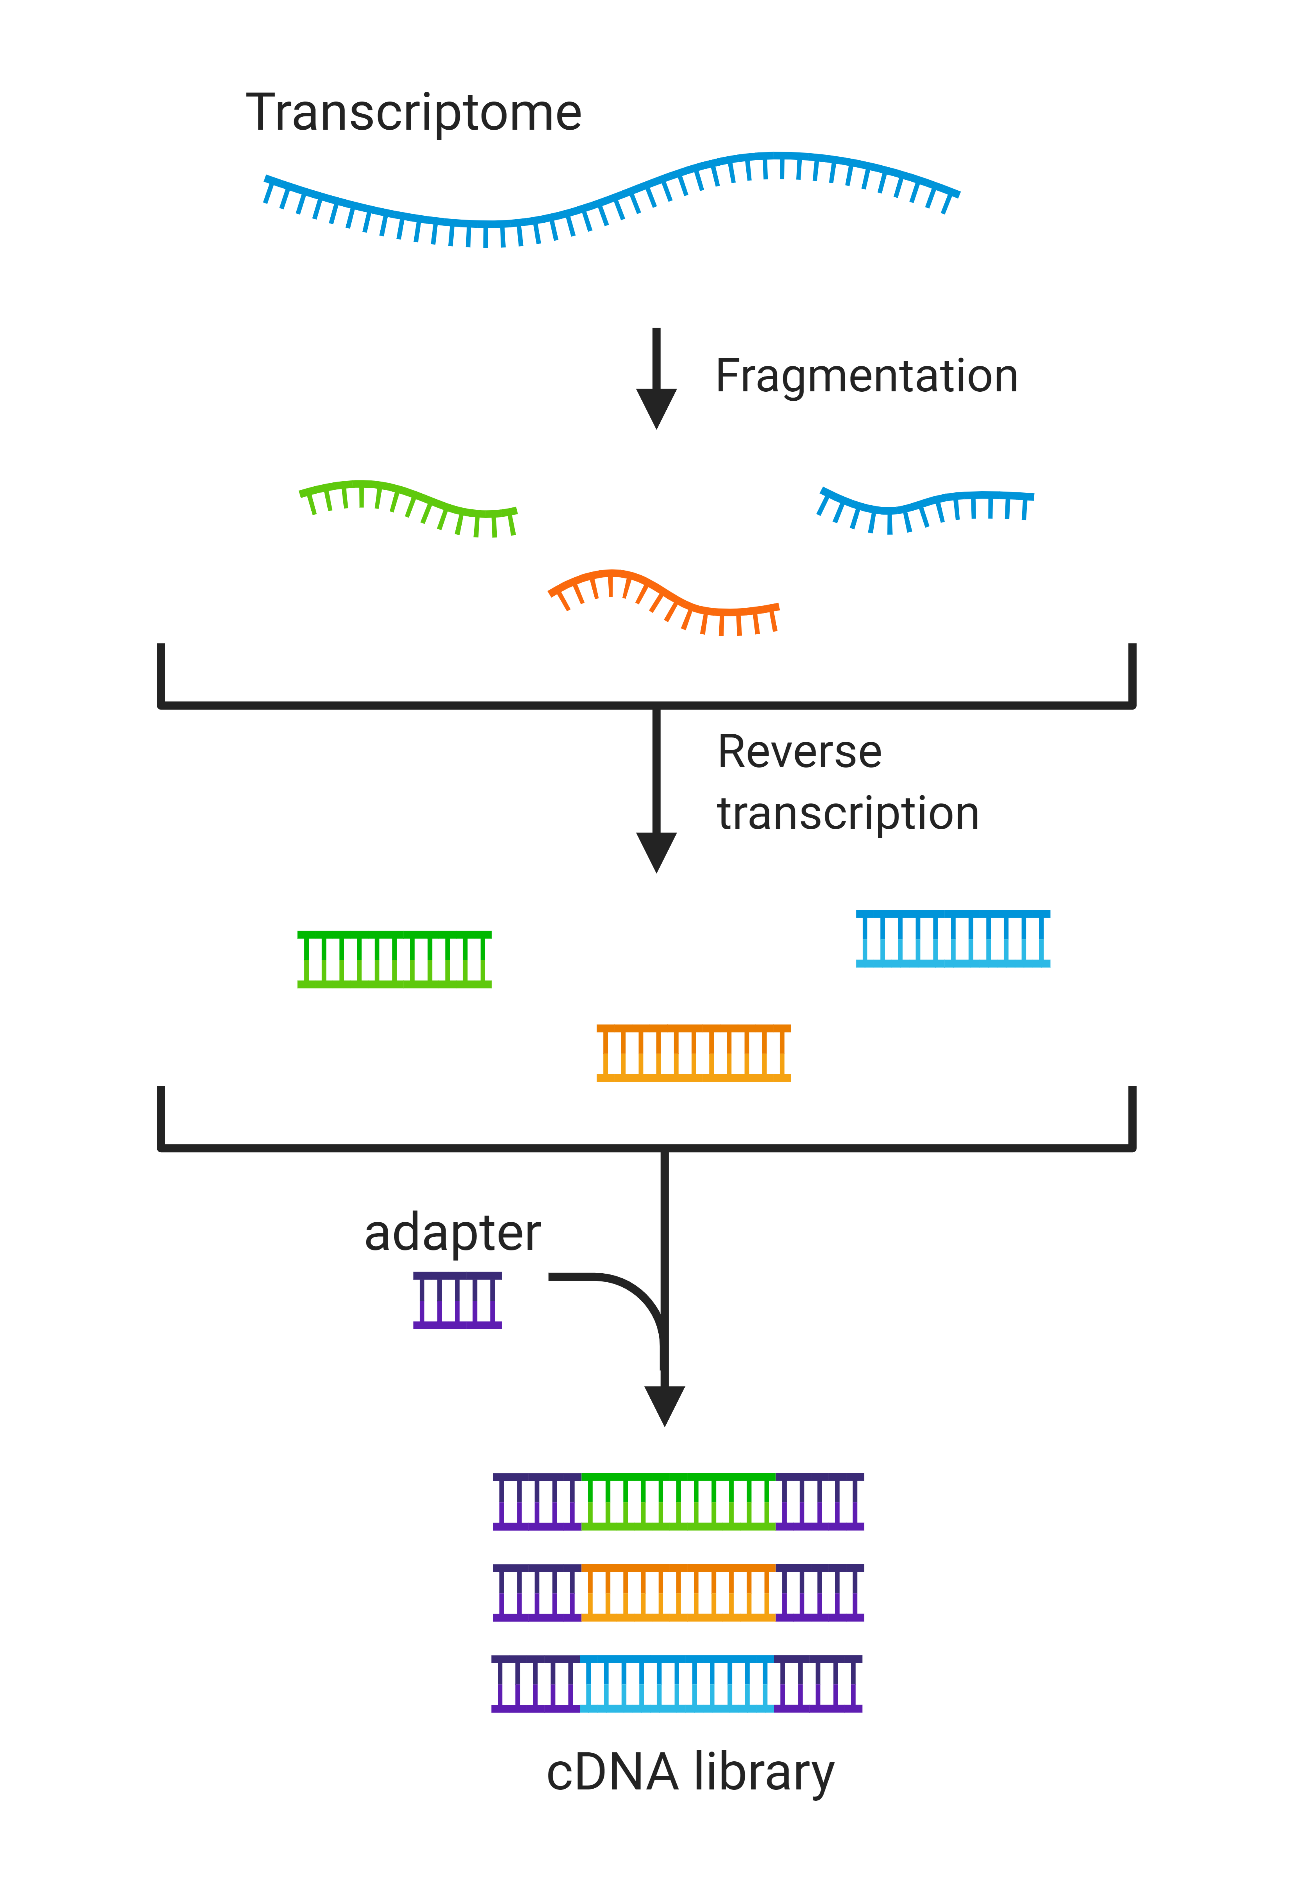
\includegraphics[width=8cm]{ngs_lib_prep}
    \caption[Library preparation]{Illumina library preparation. Created using \href{https://biorender.com/}{BioRender.com}. } 
    \label{fig:ngs_lib_prep}
\end{figure}
%\clearpage

\subsection{Clonal amplification}
The following step amplifies the fragments of the cDNA library to a level detectable by the sequencing machine, using a form of \ac{PCR}. The Illumina Sequencing by Synthesis technology makes use of the flow-cell-based method of \textit{bridge amplification} \citep{illumina2010}, as opposed to emulsion PCR, a similar technology used in Ion Torrent Semiconductor Sequencing which makes use of bead surfaces \citep{williams2006amplification}.

In bridge amplification \citep{illumina2010}, the previously prepared adapter-ligated cDNA library is attached to a flow cell, which is a hollow glass slide with multiple channels, coated with a lawn of oligonucleotides (called oligos in short) complimentary to the sequences which form part of the adapters. Strands of cDNA bind to these oligos, and polymerase creates the complement of the hybridised strand. Each double-stranded cDNA molecule is then denatured and enters a number of bridge-amplification cycles. Each molecule is amplified, forming clusters of identical cDNA sequences adjacent to each other (\autoref{fig:ngs_clonal_amp}).

\begin{figure}[!h]
    \centering
    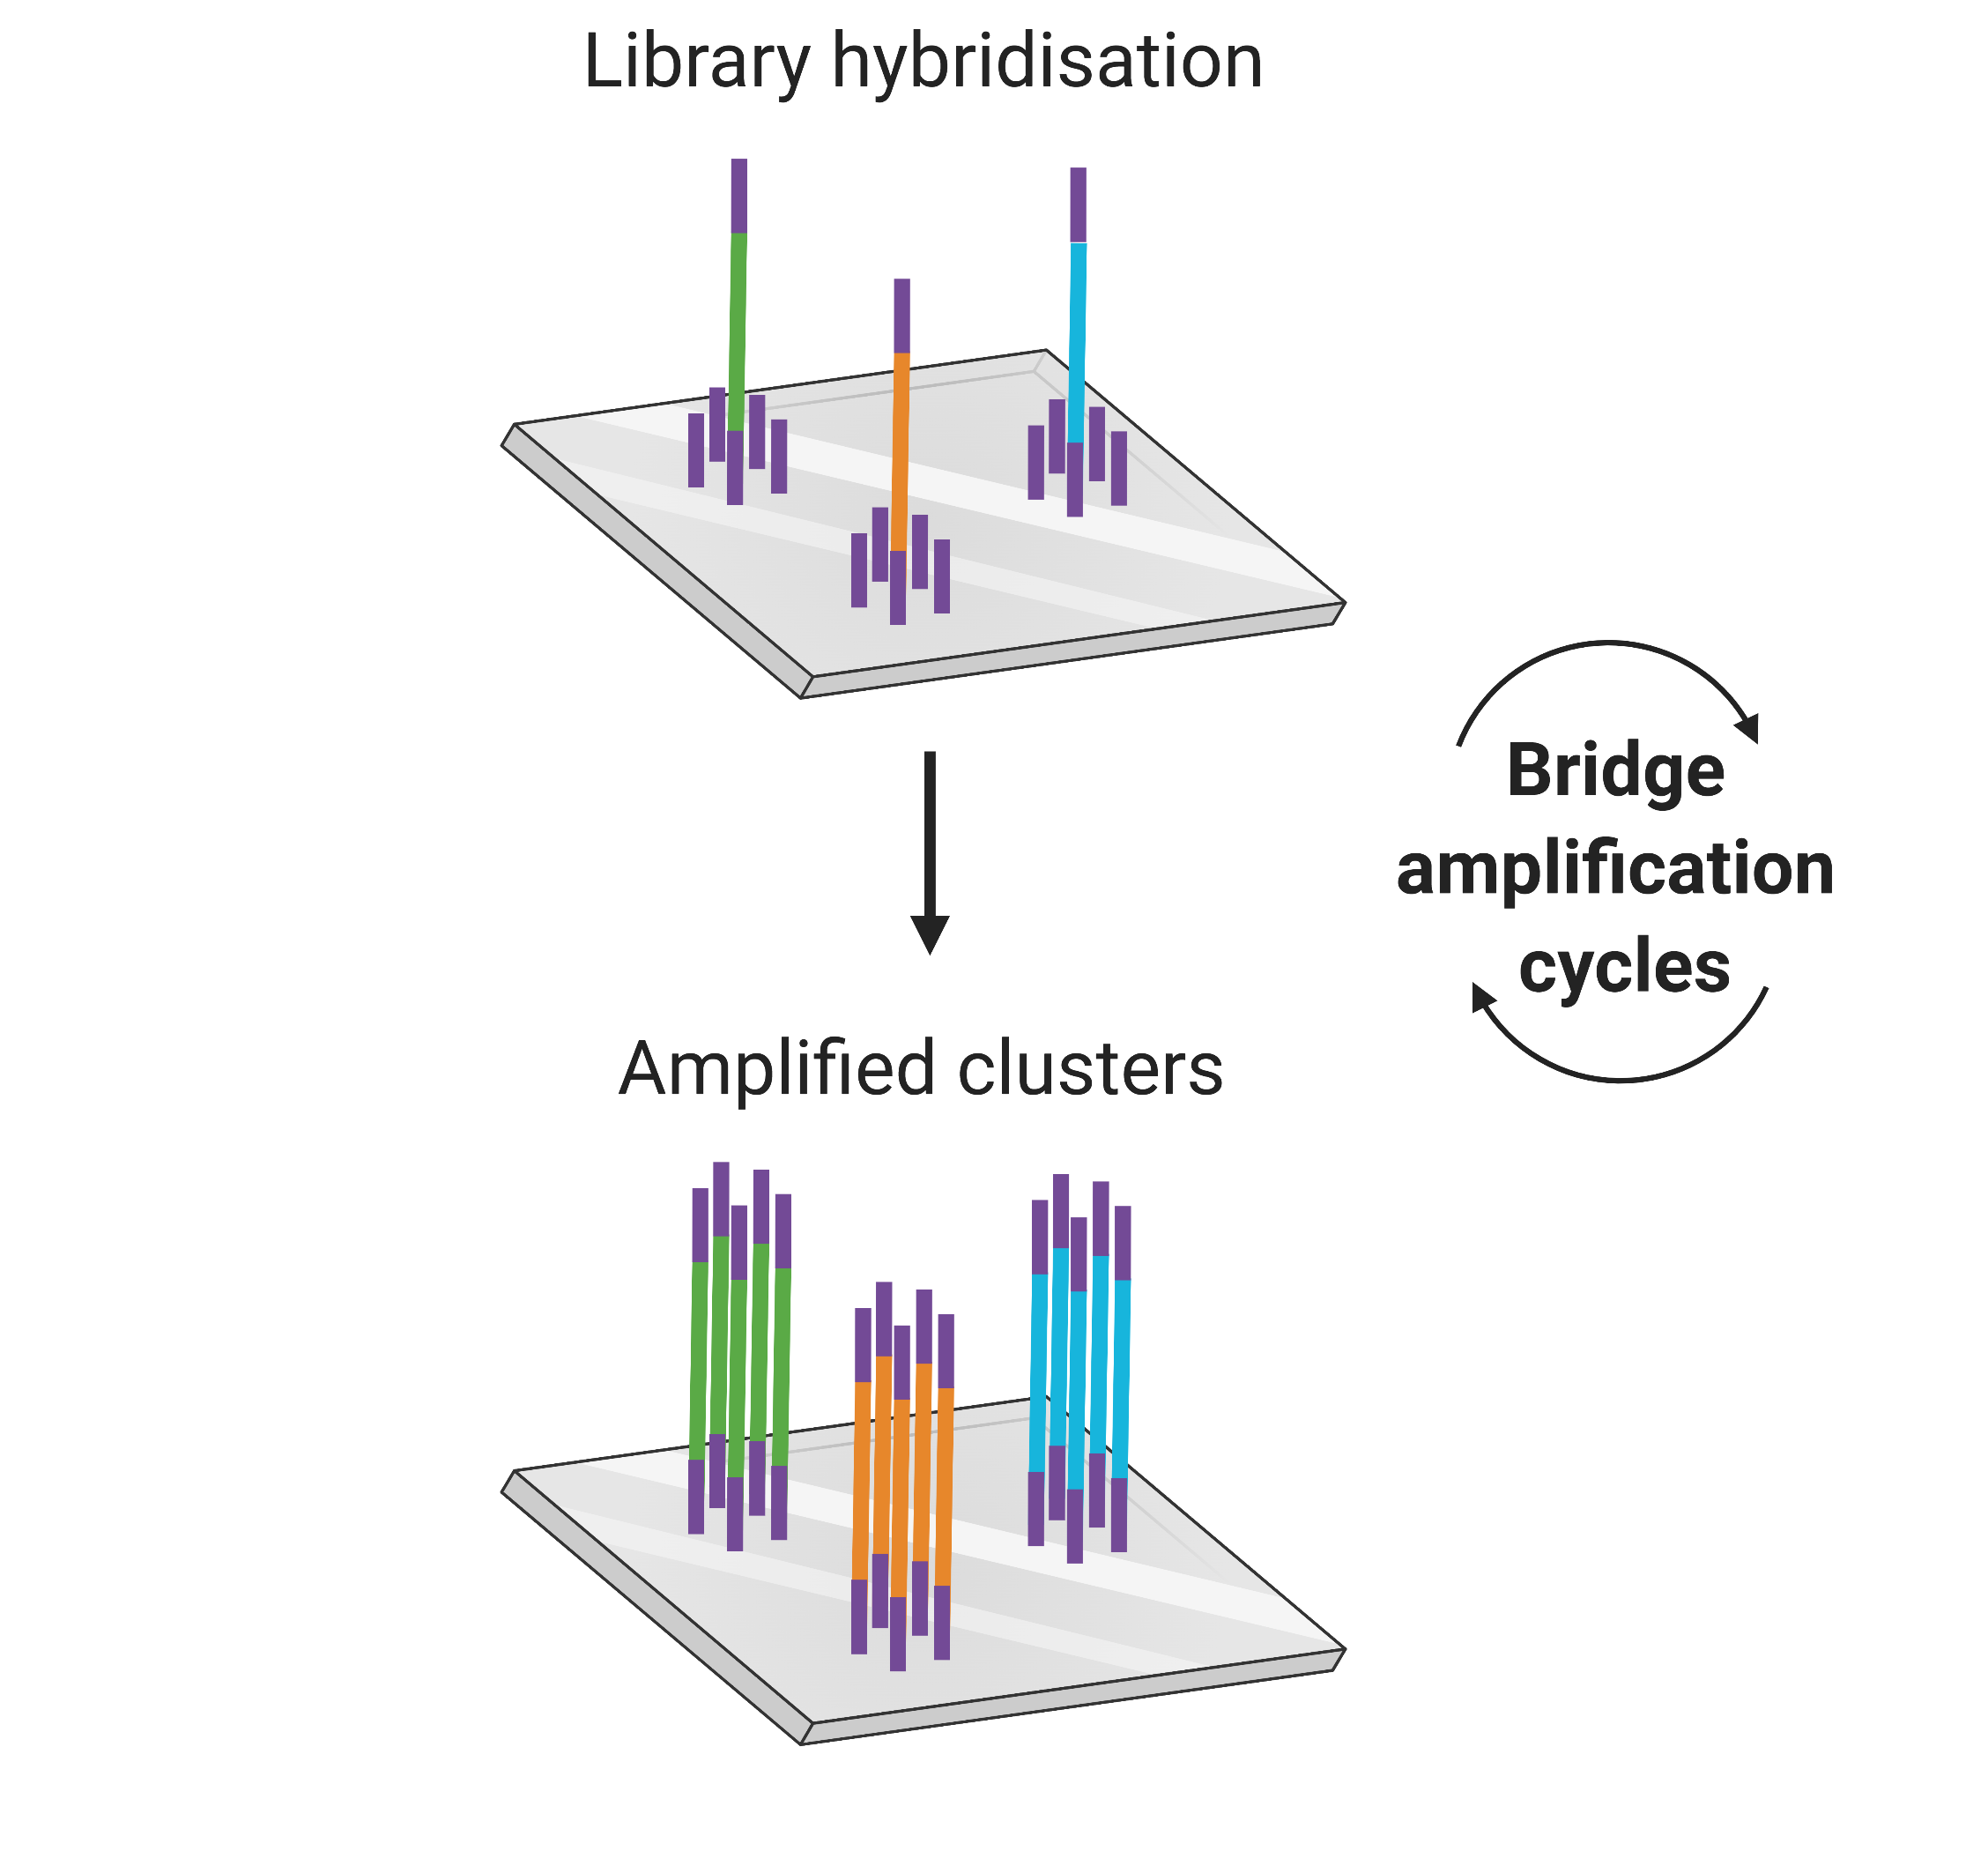
\includegraphics[width=8cm]{ngs_clonal_amp}
    \caption[Illumina clonal amplification]{Illumina clonal amplification. Created using \href{https://biorender.com/}{BioRender.com}. } 
    \label{fig:ngs_clonal_amp}
\end{figure}
%\clearpage

\subsection{Sequencing and Nucleobase Detection}
Sequencing by Synthesis \citep{illumina2010} makes use of fluorescently-labelled deoxynucleoside triphosphate (dNTP). Each sequencing cycle binds a dNTP molecule to the millions of clusters in parallel, with each of the four nucleotides emitting a different coloured light upon binding and laser excitation. The sequencing machine captures the light being emitted from the flow cell as an image and identifies the first base of each fragment. The cycle repeats itself for the second base, third base, and so on, until the end of the sequence (\autoref{fig:ngs_sequencing}). The raw sequencing data is stored as Binary Base Call (BCL) files.

Multiple samples may be sequenced simultaneously during a single run, where they are multiplexed by the machine, meaning they are pooled into a single data stream. Unique identifiers called barcode sequences (added to the cDNA fragments during library preparation) allow for the recognition of the different samples, and demultiplexing of the BCL files into text-based FASTQ files \citep{cock2010sanger}. These are immediately compressed to reduce costs associated with data storage and data transfer. While the \textit{de facto} data compression format used is gzip \citep{deutsch1996gzip}, and bzip is used on occasion \citep{seward1996bzip2}, the underlying compression algorithms used are unspecialised and inefficient for genomic data.

\begin{figure}[!h]
    \centering
    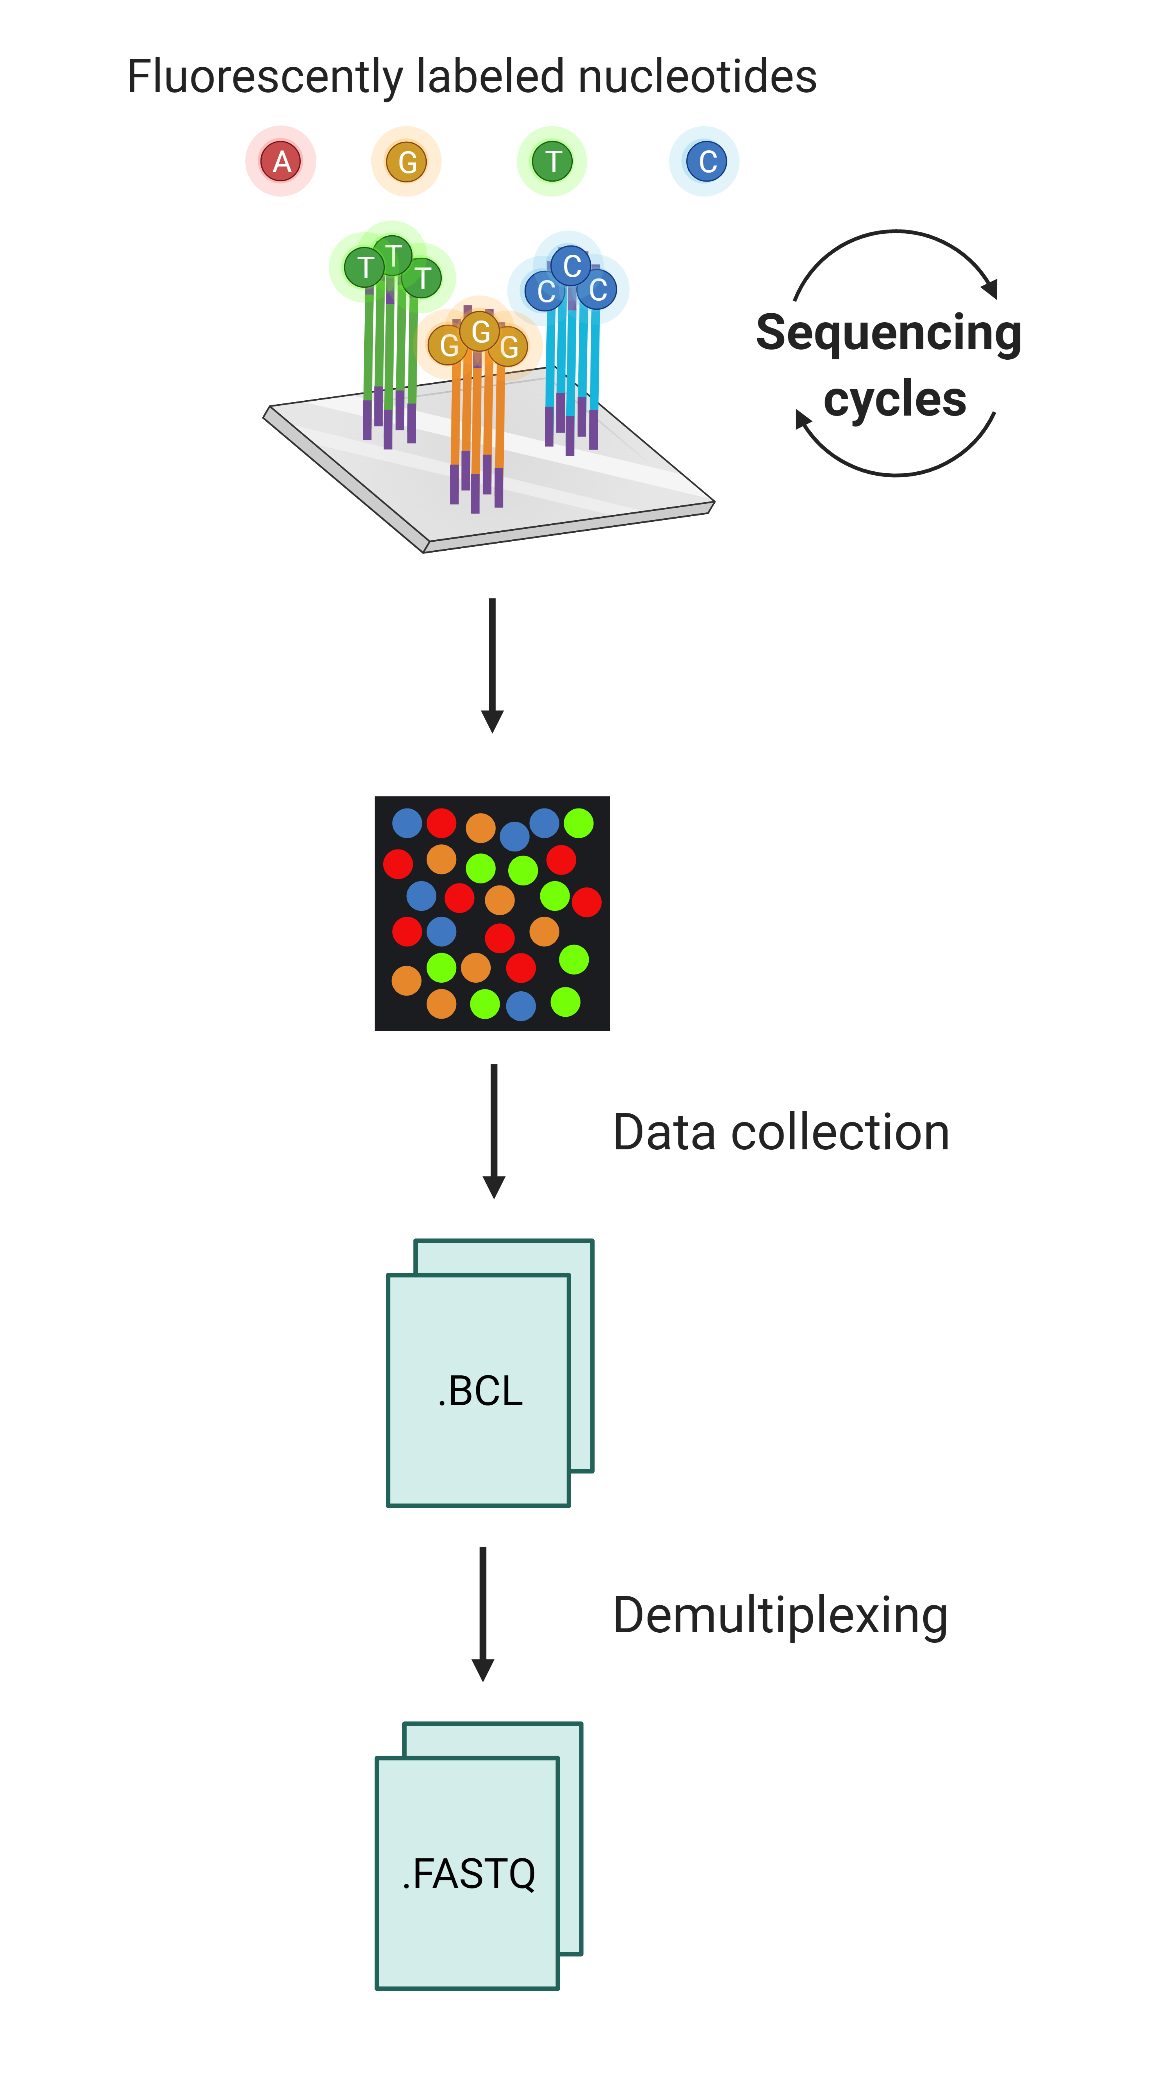
\includegraphics[width=8cm]{ngs_sequencing}
    \caption[Sequencing by synthesis]{Illumina sequencing by synthesis. Created using \href{https://biorender.com/}{BioRender.com}. } 
    \label{fig:ngs_sequencing}
\end{figure}
%%\clearpage

%illumina sequencing steps: https://www.illumina.com/documents/products/techspotlights/techspotlight_sequencing.pdf
% Potential sequencing errors

%Low complexity regions
%Sequencing software which cannot determine the nucleotide in a particular position, often represent the ambiguous base as 'N'. 
%Potential sequencing errors

% paired end vs single end: Paired-end sequencing sequences both the 5’ and 3’ end of each fragment
% read length
% coverage


\clearpage
\section{RNA-seq: \textit{in silico}}
\label{RNA-seq: in silico}

Once the FASTQ files emerge from the sequencing machines, we may move into the dry lab and feed the data into an RNA-seq data analysis pipeline. While the specific tools which make up the pipeline will vary according to the type of data and goals of the researcher, RNA-seq pipelines share a common skeleton. The following subsections will first provide a general overview of the respective step in the pipeline, and then delve into the specific tools used in this project. They were inspired by a multitude of online tutorials and resources:

\begin{itemize}\itemsep-0.5em
\item \url{https://chagall.med.cornell.edu/RNA-seqcourse/} (Last accessed 29/05/22)
\item \url{https://training.galaxyproject.org/training-material/topics/transcriptomics/tutorials/rb-RNA-seq/tutorial.html} (Last accessed 31/05/22)
\item \url{https://btep.ccr.cancer.gov/wp-content/uploads/RNA-seq_BETP_2019rev.pdf} (Last accessed 04/06/22)
\item \url{https://www.bioconductor.org/packages/devel/bioc/vignettes/DEGreport/inst/doc/DEGreport.html} (Last accessed 04/06/22)
\item \url{https://training.galaxyproject.org/training-material/topics/sequence-analysis/tutorials/quality-control/tutorial.html} (Last accessed 04/06/22)
\item \url{https://chagall.med.cornell.edu/RNA-seqcourse/Intro2RNA-seq.pdf} (Last accessed 10/06/22)
\end{itemize}

%Introns are spliced out of the pre-mRNA to form a mature mRNA transcript

\subsection{Quality Control}

The first part of any sequencing pipeline should be to analyse the quality of the data received from the sequencing machine. If poor quality sequencing information is identified, it is truncated to mitigate inaccuracies in the downstream pipeline. 

Some imperfections and uncertainties in sequencing are unavoidable, thus the reading of each base call by the sequencer is assigned a Phred quality score. The Phred score, \textit{Q}, generally ranges from 10 to 60, and is logarithmically related to the probability of an erroneous base-call, \textit{P}\citep{ewing1998base}. They are calculated as follows:
$$ Q = -10 log_{10}P $$
 $$P = 10^{\frac{-Q}{10}}$$

A common convention is to write the value of the Phred score after the letter \textit{Q}, so we may say that a base call with quality of Q30 has a 0.1\% chance of being erroneous. The FASTQ files used for this project are Sanger/Illumina 1.9 encoded, meaning that the assigned character to the score is equal to its value as an ASCII code + 33. So Q30 would correspond to the ASCII character with an ASCII code of 53, which is the question mark character '?' \citep{ewing1998base}. The lack of a base call is represented as an \textit{N} in place of the nucleotide.

\subsubsection{FastQC}
\begin{itemize}\itemsep-0.5em
\item[] \textbf{Citation}: 				\cite{andrews2010fastqc}
\item[] \textbf{Documentation}: 	\url{https://www.bioinformatics.babraham.ac.uk/projects/fastqc/Help/3\%20Analysis\%20Modules/l}
\item[] \textbf{Dependencies}: Java, Picard BAM/SAM Libraries (included in download)
\end{itemize}
% Useful: https://rtsf.natsci.msu.edu/genomics/tech-notes/fastqc-tutorial-and-faq/#:~:text=FastQC%2C%20written%20by%20Simon%20Andrews,on%20a%20sequence%20data%20set.
In the rapidly changing field of nucleotide sequencing, FastQC has been one of the few constants. It has become a staple quality control tool for high throughput sequencing data, accepting BAM \citep{BAM}, SAM \citep{li2009sequence} or FASTQ files as input, from which it produces an HTML-based report using a number of modules measuring various quality metrics. The software rates each of these modules using a green check-mark signifying that it 'passed' QC, a yellow exclamation mark 'warning', or a red cross 'failed'. However these flags are set to DNA sequencing standards, and have limited applicability with other types of sequencing, such as RNA-seq, where a number are expected to fail \citep{fastqctutorial2021}. These modules are thoroughly described in its documentation and summarised below. Care should be taken as the X-axis is non-uniform for a number of the produced graphs.

%Maybe add expected moduels to fail%copy paste the definitions for the modules from lit review lol
\begin{itemize} \itemsep0em
\item[] \textbf{Modules used in FastQC:}
\item \textbf{Basic Statistics} \hspace{0.2cm} Some basic information on the file: its name, type of quality score, total read count, read length and GC content.
\item \textbf{Per Base Sequence Quality} \hspace{0.2cm} The aggregated Q-scores at each position of the reads, represented by a box-plot.
\item \textbf{Per Sequence Quality Scores} \hspace{0.2cm} The distribution of mean Phred scores across the reads.
\item \textbf{Per Base Sequence Content} \hspace{0.2cm} A relative abundance line graph showing the percentage abundance of each of the four nucleotides across all the reads. 
\item \textbf{Per sequence GC content} \hspace{0.2cm} The percentage abundance of each of the four nucleotides across all the reads, overlaid on the expected distribution. 
\item \textbf{Per base \textit{N} content} \hspace{0.2cm} Percentage of bases at each position of the sequence with no base call, represented as an \textit{N}.
\item \textbf{Sequence Length Distribution}\hspace{0.2cm} Shows the distribution of sequence lengths, measured in number of base-pairs (bp). The module will raise a warning if all sequences are not the same length and an error if any of the sequences have zero length.
\item \textbf{Sequence Duplication Levels} \hspace{0.2cm} Percentage of reads in the library which come from sequences with duplication. Two overlaid lines indicate the percentages of the raw and the deduplicated libraries in a line graph.
\item \textbf{Overrepresented Sequences} \hspace{0.2cm} A list of sequences which account for $\geq$0.1\% of the total reads. These are compared to common contaminants to try identify them.
\item \textbf{Adapter Content} \hspace{0.2cm} A cumulative line graph where a sequence library adapter sequence is identified at that base position.
\end{itemize}


\subsubsection{FastQScreen}
\begin{itemize}\itemsep-0.5em
\item[] \textbf{Citation}: 				\cite{wingett2018fastq}
\item[] \textbf{Documentation}: 	\url{https://www.bioinformatics.babraham.ac.uk/projects/fastq_screen/_build/html/index.html}
\item[] \textbf{Dependencies}: Linux-based OS, Bowtie/Bowtie2/BWA
\end{itemize}

While FastQC is certainly a useful and well-maintained tool, it is not exhaustive of the possible QC metrics for FASTQ files. For this reason, other tools such as FastQScreen may be used to supplement the results.

FastQScreen maps the sample reads against the genomes of common contaminants and against that of a human for comparison using a third party alignment tool such as Bowtie \citep{bowtie}, Bowtie2 \citep{bowtie2} or BWA \citep{bwa}. A bar chart (\autoref{fig:fastqscreen_example}) and its respective data table are produced which show the percentage reads mapped for each genome, and what percentage did not map at all. With human samples, one should expect some mapping to the mouse and rat genomes, given their genetic similarities.
\clearpage
\begin{figure}[!h]
    \centering
    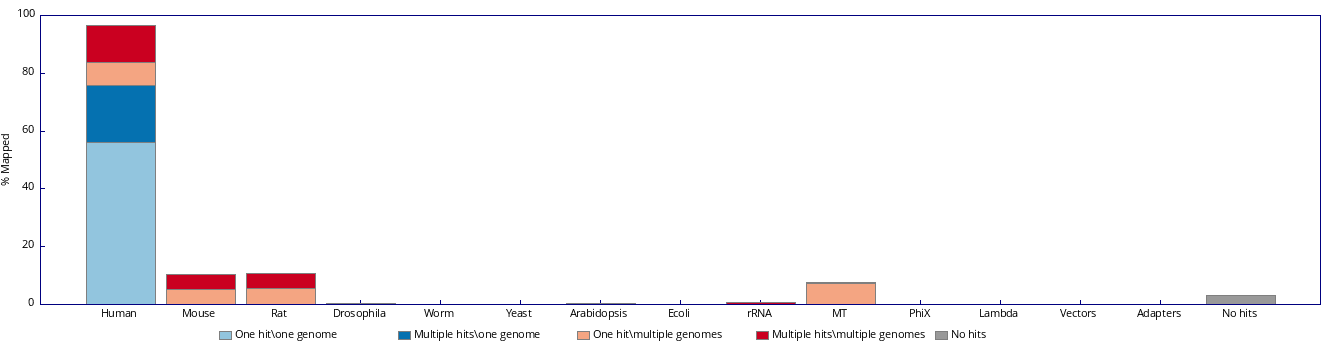
\includegraphics[width=1\textwidth]{fastqscreen_example}
    \caption[FastQScreen plot example]{An example of a good FastQScreen output result, with human mapping close to 100\% and some multi-mapping to mouse and rat genomes. } 
    \label{fig:fastqscreen_example}
\end{figure}

\subsubsection{MultiQC}

\begin{itemize}\itemsep-0.5em
\item[] \textbf{Citation}: 				\cite{multiqc}
\item[] \textbf{Documentation}: 	\url{https://multiqc.info/docs/}
\item[] \textbf{Dependencies}:  Python 3
\end{itemize}

MultiQC provides a convenient way of collating multiple QC reports across multiple samples into a single interactive HTML report. It supports the input of 114 tools as of version 1.11, including the reports from tools found further downstream, in the preprocessing, alignment or quantification parts of the pipeline. 

\subsection{Preprocessing}
If poor quality data is identified, it should be cleaned to avoid negative effects in the downstream analysis. Quality trimming which is too aggressive may similarly negatively impact downstream analysis, thus care must be taken to select appropriate quality thresholds \citep{davis2019}. Some \citep{liao2020read} doubt the necessity of trimming at all.

\subsubsection{Cutadapt: Short reads and Adapter sequences}
\label{cutadapt}
\begin{itemize}\itemsep-0.5em
\item[]\textbf{Cutadapt citation}: 				\cite{martin2011cutadapt}
\item[]\textbf{Cutadapt documentation}: 	\url{https://cutadapt.readthedocs.io/en/v4.0/guide.html}
\item[]\textbf{Cutadapt dependencies}: Python 3.7 or newer
\item[]\textbf{Trim Galore! citation}: 				\cite{trimgalore}
\item[]\textbf{Trim Galore! documentation}: 	\url{https://www.bioinformatics.babraham.ac.uk/projects/trim_galore/}
\item[]\textbf{Trim Galore! dependencies}: cutadapt, FastQC
\end{itemize}


One of the primary functions of Cutadapt (as indicated by its name) is to trim adapter sequences, which may be given as a string following the \texttt{-a} parameter. Additionally, Cutadapt may be given a read length threshold (\texttt{--length}) to remove short reads which are susceptible to multimapping and ambiguity during alignment \citep{deschamps2020handling}. 

Trim Galore! is a wrapper script that may be used to instantly redirect the trimmed reads from Cutadapt back to FastQC to reassess the data quality. It accepts the same arguments as Cutadapt, with an additional \texttt{--fastqc\textunderscore args} which accepts additional arguments to be passed on to FastQC as a string. This combines both Cutadapt and FastQC parameters into a single command. 

\begin{itemize}\itemsep0em
\item[] \textbf{Cutadapt's default options:}
\item Outputs the trimmed FASTQ file and simultaneously generates its FastQC report.
\item Assumes Sanger/Illumina 1.9 quality encoding (ASCII code +33 = Phred score)
\item Trims adapter and up- or downstream sequence
\item Allows a maximum error rate of 10 \% (Error rate = number of errors divided by length of matching region)
\item Removes up to one adapter per read
\item Requires a three nucleotide overlap between read and adapter for an adapter to be found
\end{itemize}


\subsubsection{Prinseq++: Low complexity and No Basecalls}
\begin{itemize}\itemsep-0.5em
\item[] \textbf{Short for}: 				PReprocessing and INformation of SEQuence data
\item[] \textbf{Citation}: 				\cite{prinseq++}
\item[] \textbf{Documentation}: 	\url{https://github.com/Adrian-Cantu/PRINSEQ-plus-plus}
\item[] \textbf{Dependencies}: C++
\end{itemize}
% Useful http://prinseq.sourceforge.net/manual.html
Ambiguity in reads may manifest itself in the form of low complexity regions, and reads with a high number of \textit{N}'s, in addition to those discussed in Section \ref{cutadapt}. The data should be filtered to some degree based on these metrics, which is facilitated by ready-made tools such as Prinseq++. Prinseq++ is a C++ multi-threaded implementation of the perl-coded Prinseq-lite software \citep{schmieder2011quality}. 

Regions of low-complexity (also called compositionally biased regions) are a natural part of biological sequences, playing an important role in protein translation \citep{frugier2010low}, and have a functional role in some proteins \citep{ntountoumi2019low}. Nevertheless, due to their repetitive nature, they tend to result in multimapping and low alignment confidence scores, especially when exacerbated with short read lengths. To quantify low-complexity regions, Prinseq++ present the DUST (Tatusov and Lipman, unpublished) and Entropy approaches. Both are different algorithms which employ a scoring function based on nucleotide frequencies which ultimately generate a score between 0 and 1 as a measure for sequence complexity  \citep{morgulis2006fast}. The DUST module is incorporated in BLAST \citep{altschul1997gapped} for the same purpose, to mask low-complexity regions. Prinseq++ filters reads which exceed the stipulated DUST score (\texttt{-lc\textunderscore dust}) or Entropy (\texttt{-lc\textunderscore entropy}) thresholds.

The ambiguous base \textit{N} represents no basecall, and a threshold for the maximum number of \textit{N}'s in a sequence may be set using \texttt{-ns\textunderscore max\textunderscore n}.
    
\begin{itemize}\itemsep0em
\item[]\textbf{Prinseq++'s default options:}
\item Outputs the filtered FASTQ, and the filtered reads as separate files.
\item Removes sequences with a DUST score < 0.5
\item Removes sequences with an Entropy score < 0.5 
\item Trims recursively from both ends of the sequence chunks of length 2 if the mean quality of the first 5 bases is <20 
\end{itemize}

\subsection{Alignment}

Quick and computationally efficient pairwise comparison and alignment of two sequences consisting of billions of reads is a classic problem in bioinformatics. We have amassed large volumes of literature describing potential strategies to tackle the problem, occupying different niches.

Aligners may take one of two approaches: global alignment or local alignment. Global alignment algorithms, such as \cite{needleman1970general}, aligns both sequences from their first amino acid residue through to their last and is more suitable for sequences of approximately equal lengths. By contrast, local alignment algorithms, such as \cite{smith1981identification} and BLAST, are more suited for sequences that are suspected to overlap only partially. 

There are some semantics associated with this particular step which should be clarified before proceeding further. \textit{Alignment} and \textit{mapping} are often used interchangeably, but there are subtle differences. According to the BioStar Handbook \citep{albert2020biostar}, which cites a presentation by Heng Li, \textit{alignment} is the optimal placement of a read against a genome, while \textit{mapping} suggests less certainty, and that the optimal placement is not always possible. Which term to use is dependent on the algorithm, although modern tools often combine the two approaches, which continues to blur the line separating the terms \citep{albert2020biostar}.

In RNA-seq, the reference sequence one aligns against may be either a genome or a transcriptome. Since reads from our FASTQ file originate from processed mRNA, the reads may span across multiple exons. This cannot be simply mapped onto a reference genome because of the presence of intronic and non-coding regions \citep{rnadataanalysis2020}. To map transcript-derived reads which against a genome, a splice-aware aligner must be used (\autoref{fig:alignment}).

\begin{figure}[!h]
    \centering
    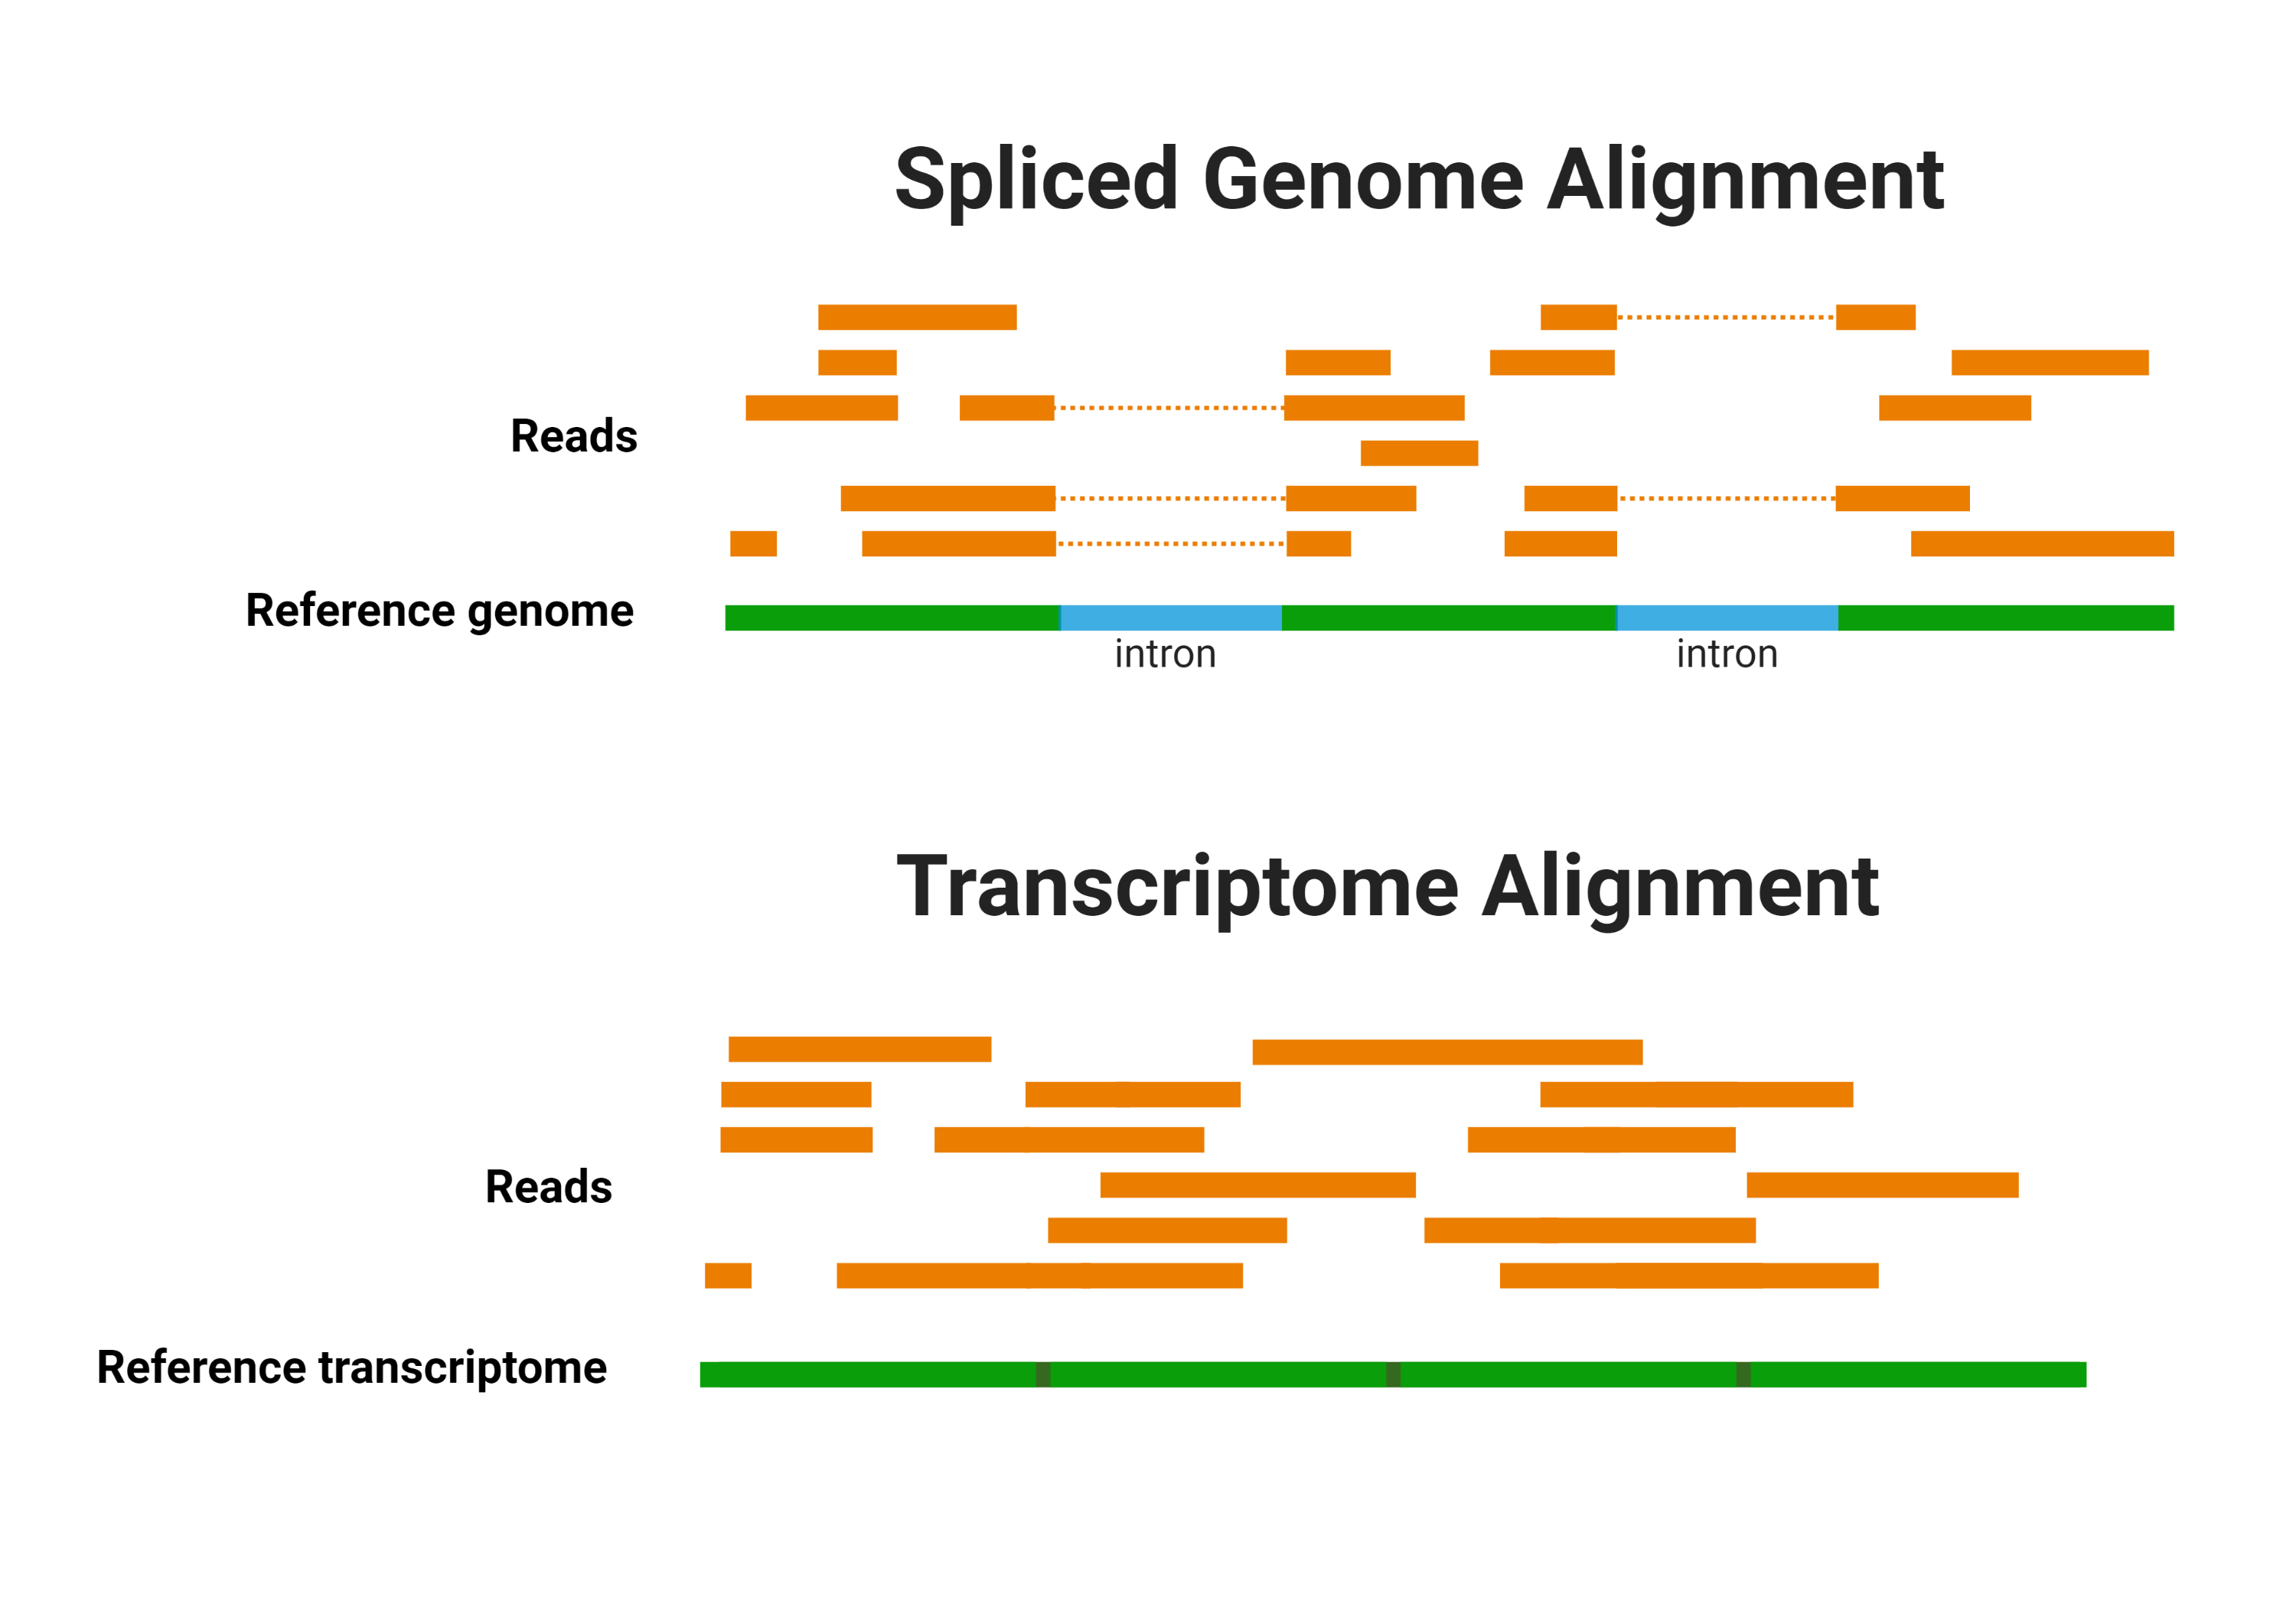
\includegraphics[width=13cm]{transcriptome_vs_genome_alignment}
    \caption[Alignment against a reference genome or a reference transcriptome]{Alignment against a reference genome or a reference transcriptome. Created using \href{https://biorender.com/}{BioRender.com}. } 
    \label{fig:alignment}
\end{figure}
%%\clearpage

Alignment algorithm efficiency is at least semi-dependent on read length, with each having ideal range of lengths, although this is rarely stated in the documentation \citep{albert2020biostar}. A distinction is often made between short-read and long-read mappers, although this distinction is arbitrary. Many conventional short-read mappers are not suitable for reads under 30bp, necessary for the study of small RNAs \citep{albert2020biostar, ziemann2016evaluation}.

Quasi-mappers and pseudo-aligners (most notably Salmon \citep{patro2017salmon} and Kallisto \citep{bray2016near} respectively) differ from classical alignment. They utilise \textit{k}-mer matching to match reads and corresponding transcripts \citep{rnadataanalysis2020}. They require less runtime than other existing alignment tools \citep{Zhang2017}, while their accuracy is disputed, with \cite{srivastava2020alignment} finding that they are less accurate and \cite{Zhang2017, Schaarschmidt2020} argue that their accuracy is comparable to conventional aligners.

Some implementation of the mapping quality (MAPQ) value is used by all conventional aligners and it is a standard field in the SAM/BAM file formats. It is analogous to the Phred score in a FASTQ file, and allows for easy filtering of bad quality reads. Unlike the Phred score, there is no single standardised definition or formula, with slight variations existing across various sources \citep{andrews2016mapq}.

%\subsubsection{The Reference Genome}

\subsubsection{STAR}
\begin{itemize}\itemsep-0.5em
\item[] \textbf{Short for}: 				Spliced Transcripts Alignment to a Reference
\item[] \textbf{Citation}: 				\cite{Dobin2013}
\item[] \textbf{Documentation}: 	\url{https://physiology.med.cornell.edu/faculty/skrabanek/lab/angsd/lecture_notes/STARmanual.pdf}
\item[] \textbf{Dependencies}: 64 bit Linux or Mac OS X
\end{itemize}

STAR is an open-source software package that performs local, splice-aware alignment in two major steps: (1) seed search and (2) clustering, stitching and scoring. It was coded in C++ for the specific purpose of mapping RNA-seq reads to a genome.
%It requires a considerable amount of RAM to run efficiently \citep{•}, and requires more runtime than Quasi-mappers and pseudo-aligners
% Suffix arrays

The algorithm first searches for the Maximum Mappable Prefix (MMP) which acts a seed from which to extend its alignment. This must be an exact identical match with the reference genome. These MMPs are clustered according to proximity to identify a set of \textit{anchor} seeds. STAR stitches together the seeds identified in the first step, and if alignment within one window does not cover the entire read, it will try to find multiple windows to cover the read, resulting in a chimeric alignment. This means that different parts of the same read may map to distant genomic loci, possibly to different strands or chromosomes, which is especially useful when dealing with cancer-derived transcriptomes given the frequency of structural variants. A local alignment scoring system guides the stitching, with matches, mismatches, indels and splice junction gaps translating to different scores.
%Perhaps a diagram here

An index must be generated prior to alignment, which is generated from a reference genome and its respective annotation file in the GTF format. This hastens the algorithm in a way similar to how one might use the index in a book, which points to the specific locations of certain headers \citep{trapnell2009map}.

STAR provides the user with great flexibility, with many parameters, such as  the scoring system weighting and the size of search windows, being user-defined. \cite{dobin2015mapping} provide excellent descriptions of nine different datatype- and output-dependent strategies that one may take when mapping RNA-seq reads with STAR. 

% perfect paper: https://currentprotocols.onlinelibrary.wiley.com/doi/abs/10.1002/0471250953.bi1114s51 
% sci hub for it: https://sci-hub.hkvisa.net/10.1002/0471250953.bi1114s51

\begin{itemize}\itemsep0em
\item[] \textbf{STAR's default options:}
\item Generates a genome index using a reference file and its respective annotation (GTF) file.
\item Aligns an experimental transcriptome using the genome index and outputs an alignment file (SAM, unsorted BAM or BAM sorted by coordinates) and various log files.
\item Uses a mapping quality metric MAPQ, calculated as $10*log_{10}(1-\frac{1}{N_{map}})$, where ${N_{map}}$ is the number of places the read maps to. A value of 255 is given to uniquely mapped reads.
\item Removes reads which map to >10 loci.
\item Passes on \texttt{NH HI AS nM} as SAM attributes as defined in the SAM format specifications\footnote{\url{https://samtools.github.io/hts-specs/SAMv1.pdf} (Last accessed 01/06/22)}.
\end{itemize}

%Multimapping:https://www.sciencedirect.com/science/article/pii/S2001037020303032

\subsection{Quantification}
\label{quantification}
% Detailed paper: https://arxiv.org/pdf/1104.3889v2.pdf
The following step associates the aligned reads with the respective genes or transcripts found at their locus. The counts of the mapped reads are proportional to the cell's expression of that particular gene/transcript. Quantifying at the transcript-level is more detailed than the gene-level, but not all research questions require this level of detail. The final output of the combined samples should be a table resembling \autoref{tab:read_count}.

\cite{pachter2011models} provides a detailed (albeit slightly outdated) review of the mathematical models behind transcript quantification, such as the Expectation–Maximization (EM) algorithm, and how they affect downstream analyses. EM estimates the maximum likelihood of proper alignment in the presence of latent variables \citep{brownlee2019gentle, pachter2011models}.

\begin{table}[h]
\centering
\caption{An example of a read count table, values representing the number of reads aligned to that gene. In bulk RNA-seq, each sample represents the pooled RNA of a large number of cells, most likely of different cell types.}
\label{tab:read_count}
\begin{tabular}{lllll}
\textbf{Genes} & \textbf{Sample$_{1}$} & \textbf{Sample$_{2}$} & \textbf{Sample$_{3}$} & ...  \\
A2BG  & 10      & 30      & 0       & ...  \\
AML   & 30      & 3       & 3       & ...  \\
AMT2  & 0       & 0       & 10      & ...  \\
ARST5 & 5300    & 1900    & 3250    & ...  \\
...   & ...     & ...     & ...     & ... 
\end{tabular}
\end{table}

\subsubsection{RSEM}
\begin{itemize}\itemsep-0.5em
\item[] \textbf{Short for}: RNA-Seq by Expectation Maximization
\item[] \textbf{Citation}: 				\cite{li2011rsem}
\item[] \textbf{Documentation}: 	\url{http://deweylab.github.io/RSEM/README.html}
\item[] \textbf{Dependencies}: 64 bit Linux/Mac OS, C++, Perl, R, STAR/HISAT2/Bowtie2
\end{itemize}

RSEM uses a statistical model based on \cite{li2010rna}, an implementation of the EM algorithm to address the issue of ambiguous read mapping, and assign reads to their appropriate gene or transcript. RSEM gives the user the option to produce both, and normalises the counts in the process. For each sample, RSEM produces two tab-delimited text files: one quantified at the gene-level and another at the transcript-level. Each row of these file represents the respective gene or transcript (the transcript file is larger due to alternative splicing), with the columns including the IDs, expected counts and normalised counts (TPM and FPKM).

An aligner (STAR, Bowtie2 or HISAT2) may be called directly through RSEM, to combine alignment and quantification (and potentially normalisation) into a single step. The genome index to be used by the aligner may be generated through \texttt{rsem-prepare-reference} and the combined alignment/quantification may be performed with \texttt{rsem-calculate-expression}.

\begin{itemize}\itemsep0em
\item[] \textbf{RSEM's default options:}
\item Accepts FASTQ files as input for alignment.
\item Outputs a gene-centric file, with the following columns: \texttt{gene\textunderscore id, transcript\textunderscore id(s), length, effective\textunderscore length, expected\textunderscore count, TPM and FPKM}
\item Outputs a transcript-centric file, with the following columns: \texttt{transcript\textunderscore id, gene\textunderscore id, length, effective\textunderscore length, expected\textunderscore count, TPM, FPKM, IsoPct}
\end{itemize}

\subsection{Normalisation}

To adjust for extraneous variables which are not biologically relevant, the read counts must first be normalised. The main factors to account for are sequencing depth \citep{robinson2010scaling}, gene length \citep{oshlack2009transcript} and GC content \citep{risso2011gc}. Effective gene expression analysis should calculate the abundance of the transcripts as a fraction of the entire RNA repertoire for that particular sample. A number of methods have evolved over the years to tackle these issues. \cite{dillies2013comprehensive} and \cite{bullard2010evaluation} extensively explore the different approaches one may take. Despite their frequent misuse in published studies, within-sample comparison methods (FPKM \citep{trapnell2010transcript}, RPKM \citep{mortazavi2008mapping}, TPM \citep{li2011rsem}, Total Counts \citep{dillies2013comprehensive}) should be avoided in \ac{DGE} analysis as they only account for differences within the same sample, and not between samples \citep{dundar2015introduction, zhao2020misuse}.

\begin{figure}[!h]
    \centering
    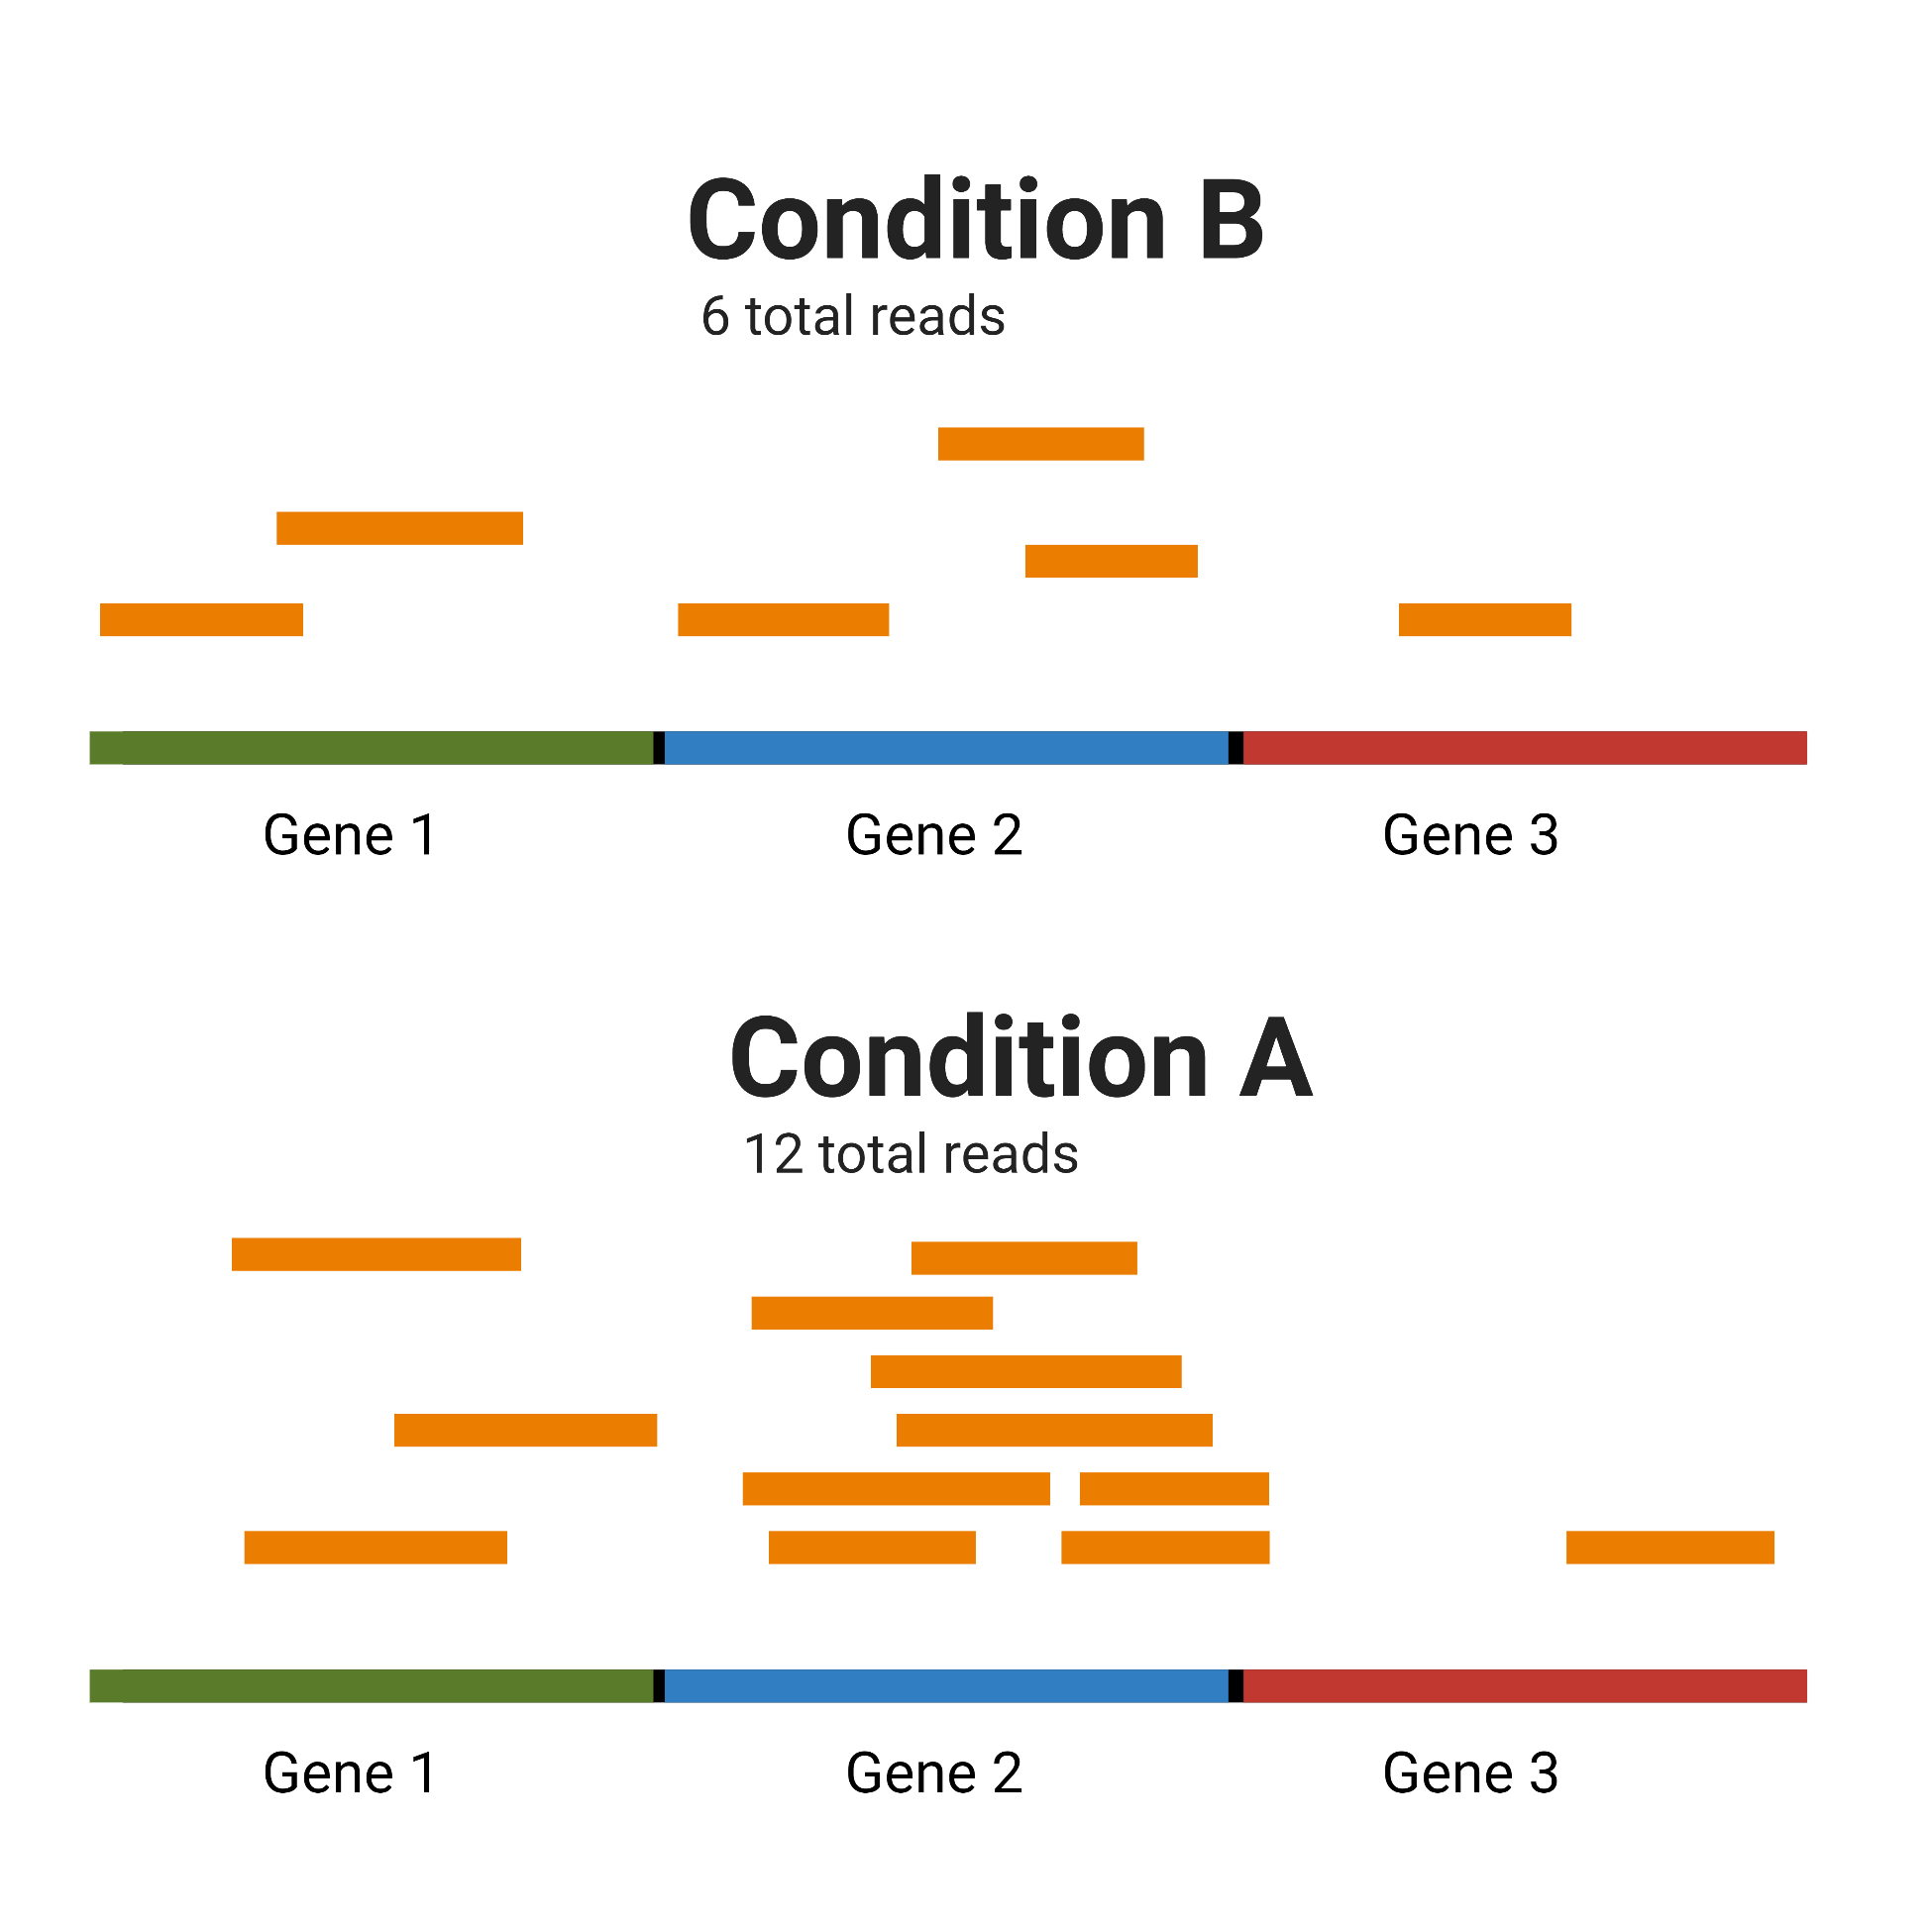
\includegraphics[width=9cm]{library_differences}
    \caption[Differences in library composition between samples]{Potential differences between samples in library composition. Condition A has more reads aligned to Gene 1 than Condition B, but it is considered more highly expressed in Condition B since the \textit{proportion} of the reads is higher. After accounting for library differences, Gene 2 is more highly expressed in Condition A, and Gene 3 is more highly expressed in Condition B. Created using \href{https://biorender.com/}{BioRender.com}. } 
    \label{fig:lib_diff}
\end{figure}
%%\clearpage

\subsubsection{Trimmed Mean of \textit{M}-values (TMM)}
\label{TMM}

The \ac{TMM} is implemented in edgeR \citep{edger} through the \texttt{calcNormFactors} function. It is recommend by the edgeR vignette\footnote{\url{https://www.bioconductor.org/packages/release/bioc/vignettes/edgeR/inst/doc/edgeRUsersGuide.pdf} (Last accessed 20/05/22)} if one wishes to continue performing \ac{DGE} analysis using that library. It was first introduced in \cite{robinson2010scaling}, who explain the underlying mathematics in detail. \ac{TMM} assumes that the majority of genes, in both samples, are not differentially expressed, although the model is robust against deviations to this assumption \citep{robinson2010scaling}. 

\ac{TMM} performs better for between-samples comparisons, as opposed to within-sample comparisons \citep{dundar2015introduction}. \cite{robinson2010scaling} recognise that it makes intuitive sense that differences in library size should be normalised (i.e. depth or coverage, as seen in \autoref{fig:lib_diff}), but they consider this scaling too simplistic for many biological applications. 

The observed counts for gene \textit{g} in library \textit{k}, calculated from the read quantification step (\autoref{quantification}), are represented as $Y_{gk}$. The total reads in library \textit{k} are represented as $N_k$. The  \textit{M}-value for gene \textit{g} and libraries \textit{k} and \textit{k'} may be calculated as:

$$ M_g = log_2 \frac{Y_{gk}/N_k}{Y_{gk'}/N_{k'}}$$

The absolute expression level, \textit{A}, for gene \textit{g} is calculated as:

$$A_g = \frac{log_2(Y_{gk}/N_k)*Y_{gk'}/N_{k'}}{2}$$

The next step is to trim the means of the \textit{M}-values and \textit{A}-values. A mean is trimmed when a percentage of the data is truncated at the upper and lower ends. By default this is 30\% for the \textit{M}-values and 5\% for the \textit{A}-values, but these settings may be changed \citep{robinson2010scaling}. 

The final step is the calculation of the normalisation factor and weighted mean of the trimmed $M_g$ using precision (inverse of the variance) weights. The calculations used in this step are beyond the scope of this project, see \cite{robinson2010scaling} for further details. % Check this with JP maybe?


\subsection{Differential Expression Analysis}
% rlly good for DGE file:///C:/Users/matth/OneDrive/Desktop/Msc%20Bioinformatics/!MMB5010%20DISSERTATION-DESKTOP-A2009SI/Literature/Tutorials/Introduction%20to%20differential%20gene%20expression%20analysis%20using%20RNA-seq.pdf 
The crux of the RNA-seq pipeline is to decide through statistical testing whether a given gene's expression varies significantly between samples, and if this variation can be explained by the difference in the cells' biology. Genes with very low read counts cannot be reliably represented across all samples, and are indistinguishable from background noise \citep{mcintyre2011rna}. These lowly expressed genes should be filtered before differential expression analysis as they are more likely to be incorrectly identified as \ac{DEG}s. All tools which measure gene expression aim to estimate two metrics  based on normalised read counts from replicated samples: 

\begin{enumerate}\itemsep-0.5em
\item The \textit{magnitude} of the differential expression, represented as the \ac{logFC}.
\item The \textit{significance} of the difference, represented as a \textit{p}-value adjusted for multiple testing.
\end{enumerate} 

The three most commonly used tools for \ac{DGE} judging by citation counts at the time of writing are DESeq2 \citep{love2014moderated}, edgeR \citep{edger} and limma \citep{ritchie2015limma}, which all take the same basic approach. Regression-based models are used to estimate the difference in normalised read counts for each gene or transcript of interest, which are tested for a significant difference \citep{dundar2015introduction}.

In differential expression analysis we are testing whether each gene in our list is significantly up- or down-regulated when compared to the reference sample. This test is performed for hundreds or thousands of genes, which is where we run into the multiple testing problem. With a 5\% error rate and 10,000 genes, we end up with 500 genes falsely identified as differentially expressed. To account for this risk, \textit{p}-values are adjusted based on how many tests are to be considered \citep{feise2002multiple}. The Bonferroni correction \citep{dunn1961multiple} is one such method, although considered by some \citep{feise2002multiple} to be too conservative, potentially over-correcting and inducing Type II errors (declaring a result not statistically significant when it is). Other, less conservative solutions have been proposed, such as the Bonferroni-Holm \citep{holm1979simple} or Hochberg \citep{hochberg1987multiple} techniques.

%Very low read counts cannot be reliably distinguished from background noise so these need to be filtered: https://pubmed.ncbi.nlm.nih.gov/21645359/
\subsubsection{EdgeR}
\label{EdgeR}
\begin{itemize}\itemsep-0.5em
\item[] \textbf{Citation}: 				\cite{edger}
\item[] \textbf{Documentation}: 	\url{https://www.bioconductor.org/packages/devel/bioc/vignettes/edgeR/inst/doc/edgeRUsersGuide.pdf}
\end{itemize}

The Bioconductor package edgeR allows the implementation of a wide array of statistical methods applicable to \ac{DGE} analysis. EdgeR accepts a matrix of reads normalised by \ac{TMM} as input (see Section \ref{TMM} for details). Prior to differential expression analysis, this matrix is filtered according to read counts using the function \texttt{filterByExpr} which removes genes with <10 read counts. Two primary routes may be taken using \autoref{fig:edger_options}, the classic route which involves exact tests \citep{robinson2007moderated, robinson2008small}, or the Generalized Linear Model (GLM) route, although certain features of the two may be combined. The GLM tests for \ac{DGE} are likelihood ratio tests (LRTs) \citep{mccarthy2012differential} and quasi-likelihood F-tests (QLFs) \citep{lun2016s, lund2012detecting}.

The \texttt{exactTest} function is based on quantile-adjusted conditional maximum likelihood (qCML) method. It produces a matrix of pseudo-counts\footnote{Note that the meaning of the term \textit{pseudo-counts} may change according to the context, and may be used by other studies to refer to something different.} which are designed to speed up computational analysis and not to be interpreted as regular normalised counts. The qCML method is only applicable on datasets with a single factor. The exact test for a negative binomial distribution should not be confused with Fisher’s exact test \citep{upton1992fisher}, although the two share many similarities.

GLMs are an adaptation of classical linear models to cater for non-normally distributed data \citep{dunn2018generalized}. The QLF dispersion estimate and test can be performed with the functions \textit{glmQLFit} and \textit{glmQLFTest}. This fits a negative binomial GLM to the \ac{TMM} normalised read counts. The LRT compares the goodness of fit of two competing models through the functions \textit{glmFit} and \textit{glmLRT}.

\begin{figure}[h!]
    \centering
    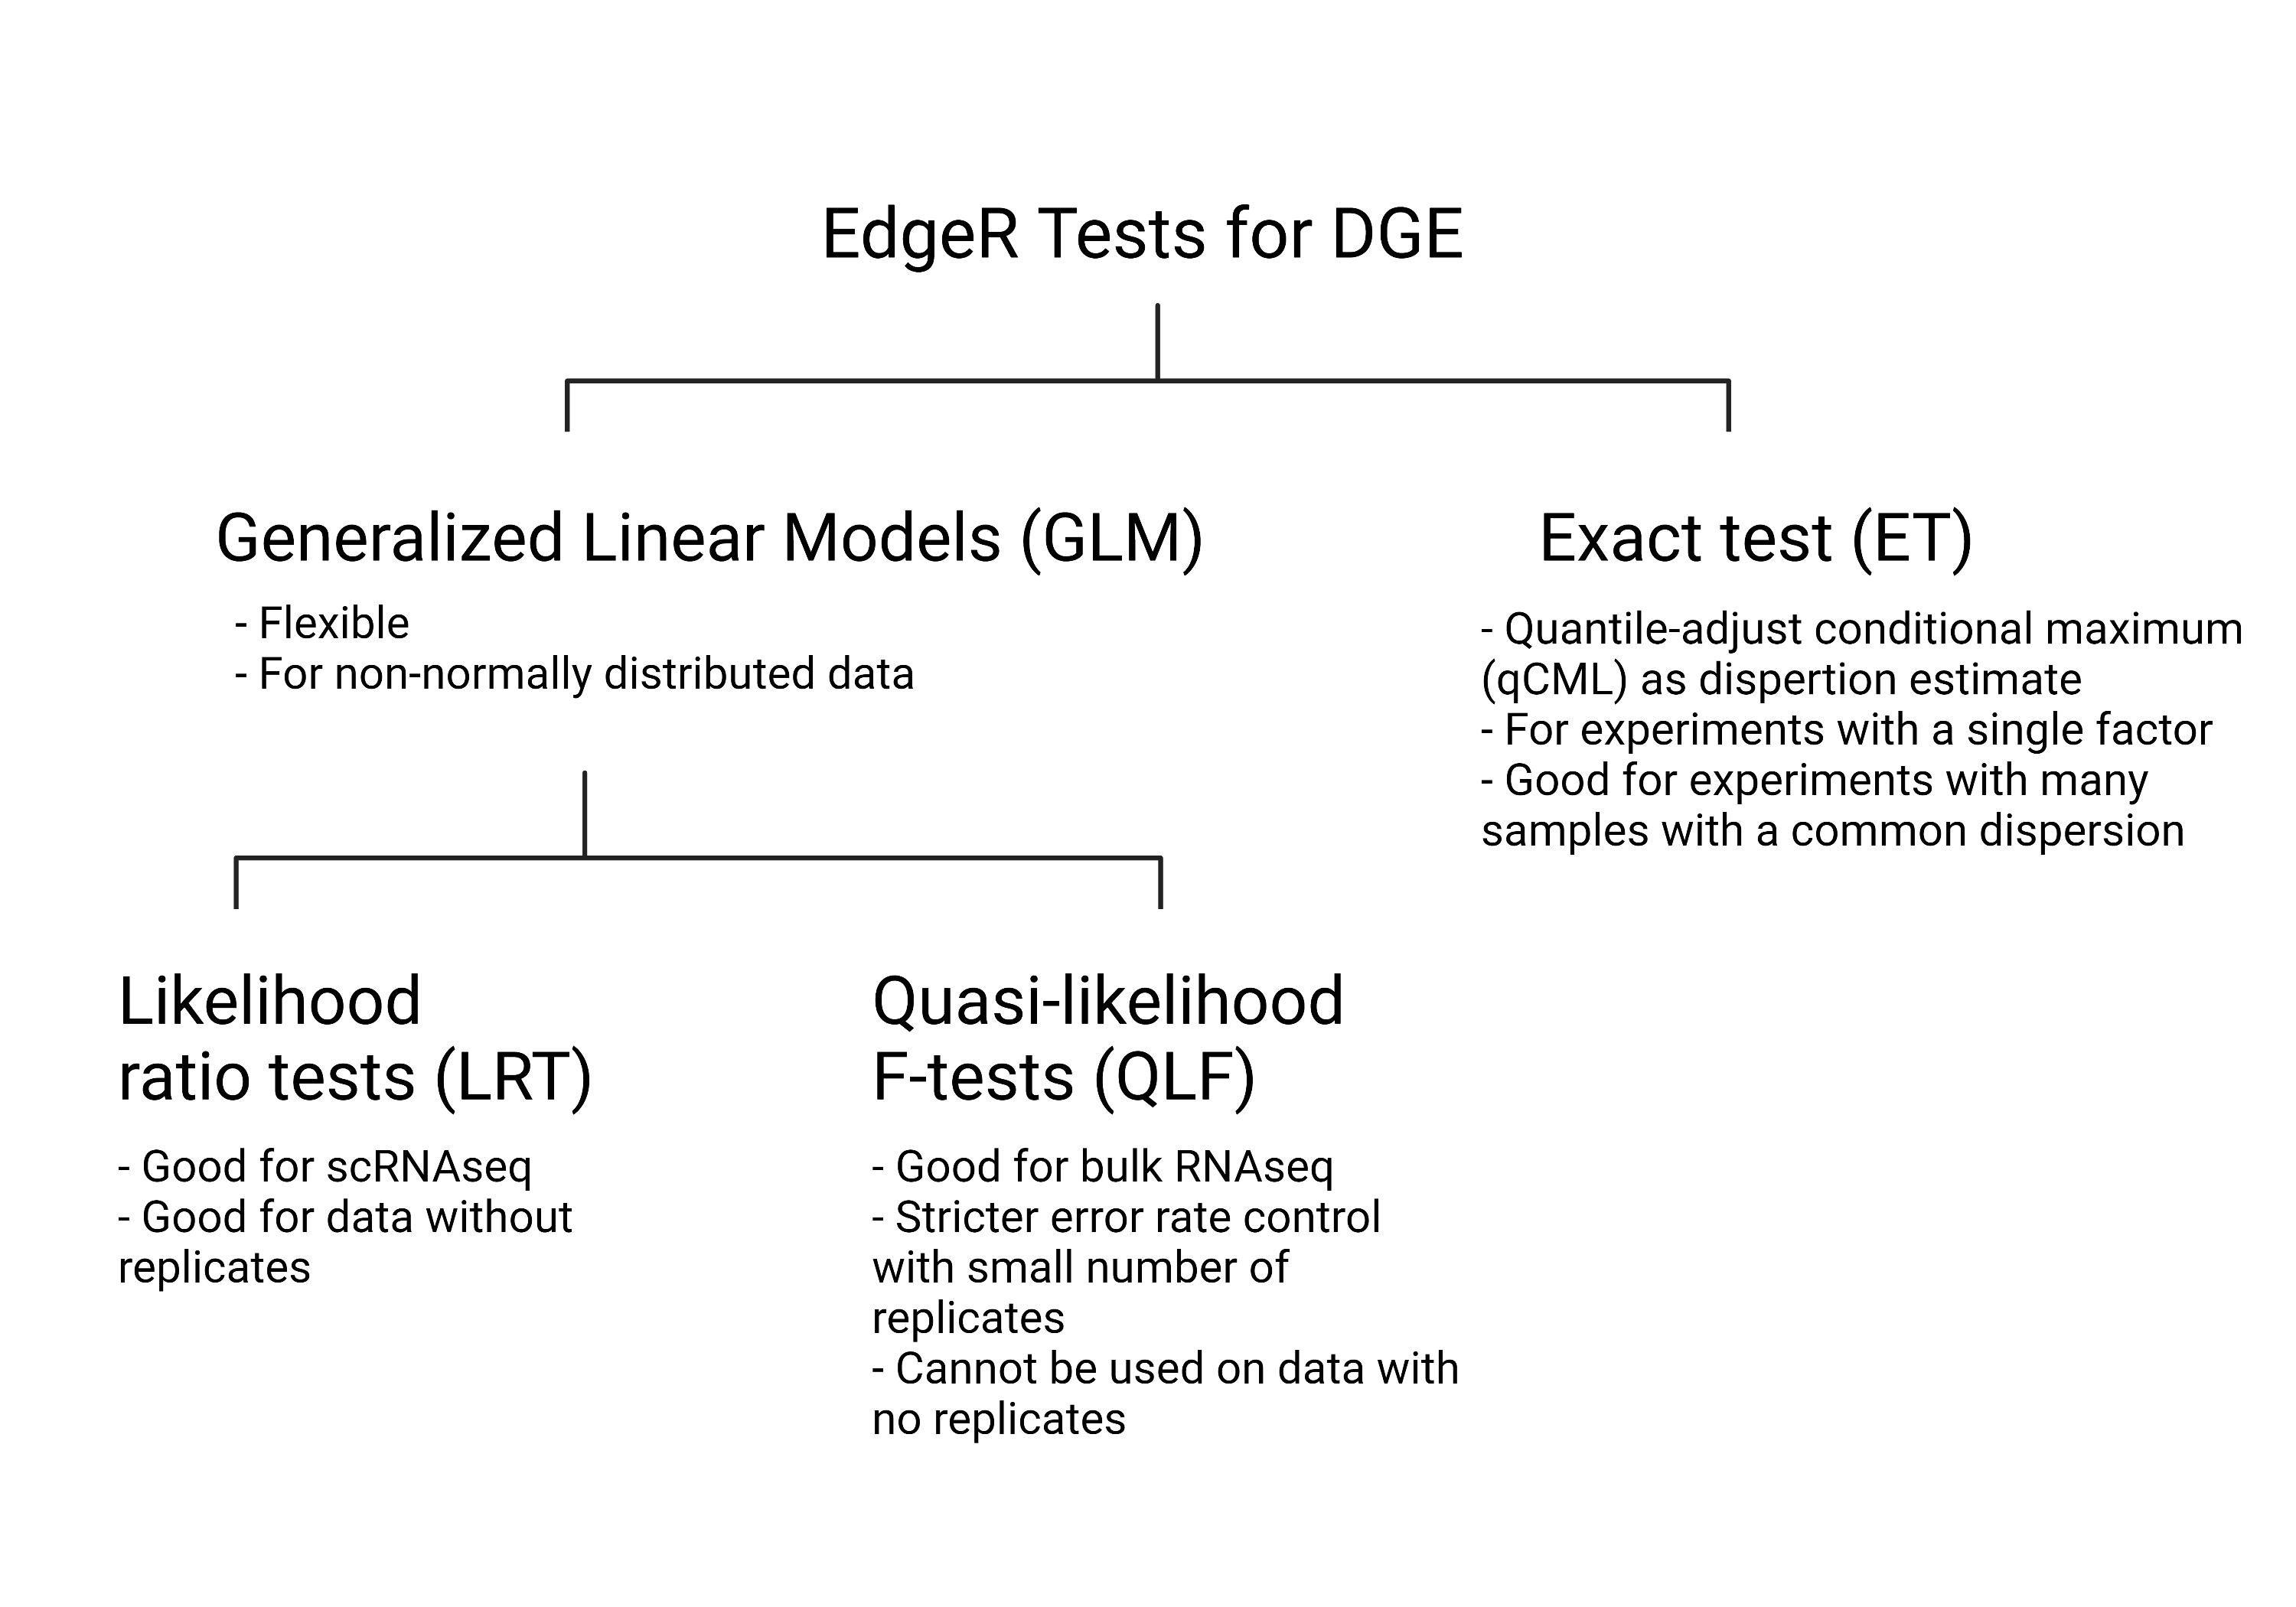
\includegraphics[width=13cm]{edger_dge_options}
    \caption[Summary of the options provided by edgeR for DGE identification]{Summary of the three options provided by edgeR for \ac{DGE} identification, based on comments and recommendations by its vignette. } 
    \label{fig:edger_options}
\end{figure}
%\clearpage

EdgeR and DESeq2 are quite similar in that they both make use of a negative binomial distribution to model read counts, and estimate dispersion based on the approximate conditional inference, first proposed by \cite{cox1987parameter}.  EdgeR is recommended for experiments with fewer than 12 replicates \citep{schurch2015evaluation}, and unlike DESeq2, allows for the analysis of data with no replicates, although highly discouraged by the vignette. 
% The negative binomial is a more general form of the Poisson distribution... maybe write some shit on this

The biggest challenge when working with data without replicates is the estimation of dispersion, which is mathematically impossible given a single sample. In cases when there is no other alternative, the vignette suggests giving a nominal value to the \ac{BCV}, from which we may derive the dispersion. The vignette suggests a few estimates for the \ac{BCV} which are based on previous experiments as the dispersion, such as \textit{0.1 for data on genetically identical model organisms}. The dispersion is equal to this value squared, which although inaccurate, is a better alternative to assuming no variance.

To account for the previously described multiple testing problem, the \texttt{topTags} function adjusts \textit{p}-values using the Benjamini-Hochberg method \citep{benjamini1995controlling} to control the \ac{FDR}. This produced value is the proportion of false positives one might expect to get from a test. %more detail

To gain further biological insight, the \texttt{goana} and \texttt{kegga} functions may be used to annotate genes according to their associated \ac{GO} terms and \ac{KEGG} pathways respectively. This may be particularly useful in downstream tests for gene set analyses.

The end result should be an edgeR object containing a matrix of each the \ac{logFC}, adjusted \textit{p}-values and (optionally) annotations for each differentially expressed gene. The final step is filtering on the matrix by setting a (largely arbitrary) \ac{logFC} and/or \textit{p}-value cutoff, and sorting the data by one of these metrics for easier biological analysis.
% Visit later and suggest values

\subsection{Downstream Analysis}
% alternative splicing, functional analysis, gene fusion detection and eQTL mapping
The steps of the pipeline up until this point are quite standard, although there are various approaches one may take, the aim of each step is clear and consistent across all RNA-seq studies. Further exploration of the data is highly specific to the experimental design and research question. Putting the data into its biological context is a type of sanity check. Deviation from biological expectations is often an indication of issues in the upstream analysis.

\subsubsection{Visualising Results}

Graphical representation of the gathered information about the samples thus far conveys the information in a more human-readable format and allows for easier pinpointing of differences, potential batch effects and other
errors. Descriptive statistics are helpful, but can be misleading as proven by Anscombe's quartet \citep{anscombe1973graphs}.

%Sashimi plot
\begin{enumerate}
\item[] \textbf{Multidimensional Scaling (MDS)} \hspace{0.15cm} RNA-seq data deals with thousands of dimensions, making it difficult to interpret and impossible to use conventional plotting methods. MDS is type of non-linear dimensionality reduction used to mitigate this issue \citep{yin2007nonlinear}. It is a between-sample measure of similarity which plots pairwise distances using Cartesian coordinates \citep{mead1992review}. 

\item[] \textbf{Principal Component Analysis (PCA)} \hspace{0.15cm} Similar to MDS in scope except that it is a \textit{linear} dimensionality reduction technique. PCA transforms the data to find the combination of variables which explains the maximum variation in the data. 

\item[] \textbf{Heatmaps and Clustering} \hspace{0.15cm} Often used in combination with each other, with a colour gradient in the heatmap signifying the \ac{logFC} for each gene in the list, which are clustered according to similar expression patterns.

\item[] \textbf{Mean-Difference (MD)} \hspace{0.15cm}  In RNA-seq it is used to measure the difference between each gene's \ac{logFC} of a given sample against the mean \ac{logFC} of that respective gene. In other fields, it is used to determine if two methods of measurement are in agreement \citep{fry2008visualizing}.

\item[] \textbf{Volcano Plot} \hspace{0.15cm} Plots the results of differential expression that plots the significance (adjusted \textit{p}-values) against the \ac{logFC}. Thresholds of each are often indicated by a change in colour of the points.
\end{enumerate} 

%Include some examples?

\subsubsection{Annotation and Enrichment Analyses}

The differentially expressed gene matrix may be annotated using the AnnotationDbi \citep{annotationdbi} R package which may access annotation libraries such as the human org.Hs.eg.db \citep{org.Hs.eg.db} which is based on Entrez gene identifiers \citep{maglott2005entrez}. The systems biology of the data is of particular interest to this project, which may be investigated with enrichment analyses. % or STRING \citep{szklarczyk2016string}
\ac{GO} terms and \ac{KEGG} \citep{kanehisa2017kegg} pathway enrichment allow for comparisons between genes according to their functional role in a biological system. Further enrichment analyses may fork into three approaches, as described by \cite{khatri2012ten} and \cite{alhamdoosh2017combining}:

\begin{enumerate}
\item[] \textbf{\ac{ORA}} \hspace{0.15cm} The gene list emerging from differential expression is compared to a list of genes associated with a specific pathway. The genes which overlap between the input list and the pathway list are tested for over- or under-representation (usually based on hypergeometric, chi-square, or binomial distribution) \citep{khatri2012ten}. While this information is useful, ORA is limited in that it only tests for the presence of a gene, and ignores any additional information (\ac{logFC}s, \textit{p}-values, the effect of its products on other genes, etc.).

\item[] \textbf{\ac{GSEA}} \hspace{0.15cm} The limitations to the ORA approach led to the development of an alternative method, GSEA. The philosophy behind \ac{GSEA} is that although large fold-changes in individual genes can have a significant biological effect, so can weaker changes in genes with a disproportionate effect on the pathway. \cite{luo2009gage} describe the term \textit{gene set} as a pre-defined group of functionally related genes, which may share a common biological pathway or ontology term. \ac{GSEA} is generally performed in three steps: (i) generation of gene-level statistics (e.g. ANOVA) which may be transformed (e.g. absolute values), (ii) statistical results are combined into a single value per gene set (e.g. Wilcoxon rank sum \citep{barry2005significance}) and (iii) the statistical significance of the gene-set-level statistic are assessed. Although an improvement over the previous method, \ac{GSEA} treats gene sets separately and does not consider that a gene may be involved in multiple sets.

\item[] \textbf{\ac{PTA}} \hspace{0.15cm} Building upon the previous two technologies, \ac{PTA} approaches take into account interactions between gene products, and the nature of their interaction (e.g. activation or inhibition). KEGG and STRING \citep{szklarczyk2019string} are examples of knowledge-bases which have sufficient information to perform \ac{PTA}. There are several potential approaches which are difficult to generalise but are reviewed extensively in \cite{ihnatova2018critical} and \cite{ma2019comparative}.
\end{enumerate} 
% good resource: https://ressources.france-bioinformatique.fr/sites/default/files/4%20-%20FGSA_Roscoff.pdf


\subsubsection{GAGE}
\begin{itemize}\itemsep-0.5em
\item[] \textbf{Short for}: 			Generally Applicable Gene-set Enrichment
\item[] \textbf{Citation}: 				\cite{luo2009gage}
\item[] \textbf{Documentation}: 	\url{https://bioconductor.org/packages/devel/bioc/vignettes/gage/inst/doc/gage.pdf}
\end{itemize}
% https://bioconductor.org/packages/release/bioc/vignettes/gage/inst/doc/RNA-seqWorkflow.pdf

GAGE performs \ac{GSEA}, where gene-set-level statistics are generated to check which gene sets are differentially expressed. %revsit 
GAGE performs pair-wise comparison between samples by default to test for significantly differentiated \ac{KEGG} and \ac{GO} gene sets. This is performed in three steps:

\begin{enumerate}
\item \textbf{Input preparation} \hspace{0.15cm} Gene sets are separated into two categories: experimental sets and canonical pathways.
\item \textbf{Gene set differential expression} \hspace{0.15cm} Test whether each gene set is significantly differentially expressed using a two-sample t-test.
\item \textbf{Summarisation} \hspace{0.15cm} A \textit{p}-value, an \ac{FDR} \textit{q}-value and a test statistic are derived for each gene set. The test statistic gives an indication of the direction of regulation of the set.
\end{enumerate} 

Pathview \citep{luo2013pathview},is a Bioconductor \citep{gentleman2004bioconductor} R package which visualises GAGE results as an image of the chosen KEGG pathway highlighting the differentially expressed genes according to their \ac{logFC}s. Its sister library SBGNview \citep{dong2022sbgnview} offers a wider array of gene set knowledge-bases such as PANTHER \citep{mi2005panther}, Reactome \citep{croft2010reactome} and SMPDB \citep{frolkis2010smpdb}. Pathview supports two methods for pathway visualisation: the native KEGG view and the third party Graphviz \citep{ellson2001graphviz}. \cite{luo2013pathview} states that Graphiz provides better control over the graphical nodes and edges, at the expense of certain pathway metadata, namely cell types and temporal information.

\ac{GO} term analysis is supported by GAGE, although frequently neglected due to the popularity of \textit{pathway} analysis as opposed to the more generalised \textit{gene set} analysis \citep{luo2009gage}. Since \ac{GO} terms do not contain information on molecular interactions, pathways similar to those constructed by Pathview are not an option. The data may be represented by heatmaps or scatterplots as arguments in the \texttt{geneData} function.

%Include pathview image?

\clearpage
\section{Evaluation Criteria}
Every step in the pipeline is followed by some form of QC and potentially filtering of bad data, from trimming adapter sequences to filtering multimapped reads to removing very lowly expressed genes. It is not unlikely that errors of any form slip through, and for these reason the final results will be evaluated.

The list of \ac{DEG}s will be checked against a list of housekeeping genes which will act in a similar fashion to negative controls. Housekeeping genes are required for basic cellular function and must be expressed in both normal and pathological cells. While they may be differentially expressed in some cases \citep{greer2010housekeeping}, they are generally uniformly expressed with low variance \citep{khimani2005housekeeping}. The Housekeeping and Reference Transcript Atlas (HRT Atlas) \citep{hounkpe2021hrt} was used as a source for the gene lists. % REVISIT THIS!!

Similarly, the \ac{DEG}s will be cross-checked against the results of similar studies to confirm their biological relevance. The genes and pathways affected by cancer, even those specifically affected by \ac{AML} are well studied, annotated and aggregated in repositories such as GeneCards \citep{stelzer2016genecards} or OMIM \citep{hamosh2005online}. 

In future work, if more funds are acquired, similar work could be conducted with more technical replicates to confirm the findings of this project with greater statistical power. To decrease the number of sequencing errors, Sanger Sequencing could potentially be used, given its 99.999\% accuracy rate and long read lengths of up to \textasciitilde 1000bp \citep{shendure2008next}.

\clearpage
\section{Related Work}
This multidisciplinary project is based on multiple rapidly developing fields, thus it is important to keep updated with the latest literature. This section will describe the methods and findings of literature which this project will build upon, namely those which cover: (i) the biochemical components of extra virgin olive oil and their potential application to clinical practice, (ii) compounds with chemotherapeutic potential in \ac{AML} and the resultant \ac{DEG}s and (iii) tools to construct an effective RNA-seq pipeline given our specific data.

\subsection{Biochemistry of Olive Oil}
The Mediterranean diet is rich in fruits, vegetables, fish, and olive oil, and is linked to lower rates of atherosclerosis, cancer and cardiovascular disease \citep{owen2000, tripoli2005phenolic, cicerale2012antimicrobial, fabiani2002cancer}. This is attributed in part to the higher intake of extra virgin olive oil, and more specifically, its phenolic compounds. These have been the subject of extensive investigation as a result of their antimicrobial, antioxidant and anti-inflammatory properties \citep{cicerale2012antimicrobial, tripoli2005phenolic, bendini2007phenolic, serreli2018biological}. \cite{tripoli2005phenolic} attributes olive oil's slightly bitter and pungent taste to hydroxytyrosol and oleuropein, which both exhibited antioxidant activity.

\cite{owen2000} split the biochemical profile of olive oils into three classes: (i) simple phenols (e.g. hydroxytyrosol, tyrosol), (ii) secoiridoids (e.g. oleuropein) and (iii) the lignans (e.g. pinoresinol). All three classes have shown antioxidant properties.

\cite{gatt2021first} was the first to characterise the phenolic profiles of Maltese extra virgin olive oils. Through liquid-liquid extraction and liquid chromatography mass-spectrometry, they found that the major constituents are tyrosol, hydroxytyrosol (\autoref{fig:tyrosol_hydroxytyrosol}) and their derivatives. This is in accordance with olive oils from other sources (\citep{Angerosa1995}), although the compound concentrations may vary. These two classes of simple phenols have been the main focus of clinical research related to olive oil extracts.

\begin{figure}[!h]
    \centering
    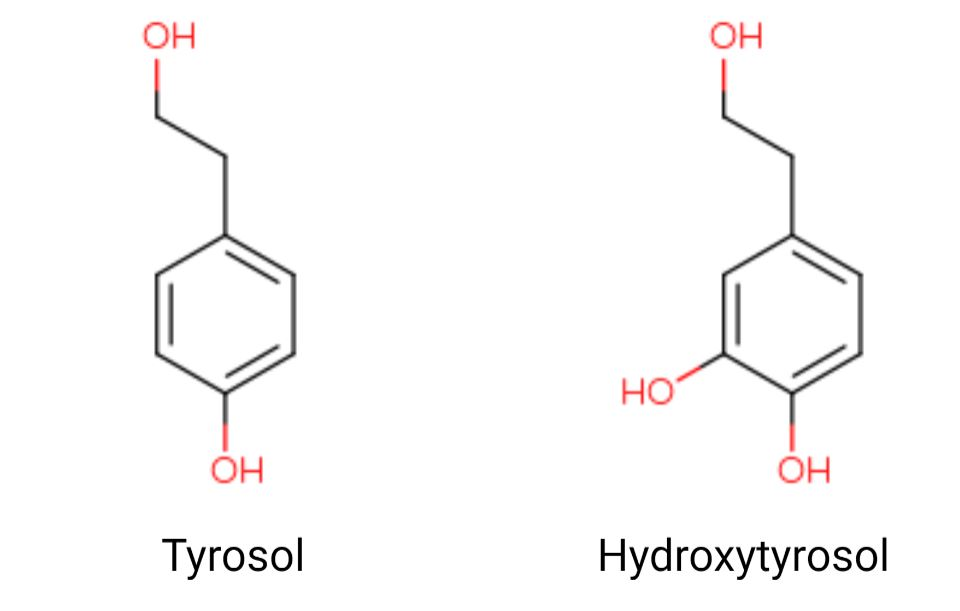
\includegraphics[width=8cm]{tyrosol_hydroxytyrosol}
    \caption[Chemical structures of tyrosol and hydroxytyrosol]{Chemical structures of tyrosol and hydroxytyrosol. The rest of the phenolic profile of extra virgin olive oils consists of derivatives of these two compounds.} 
    \label{fig:tyrosol_hydroxytyrosol}
\end{figure}


There is abundant literature on the role of natural phenolic compounds in general in the prevention and treatment of cancer. This is achieved by regulating the cell cycle \citep{jafari2014role} and the epigenome \citep{pan2015breast}. These compounds may complement traditional chemotherapeutic treatments, potentially lessening the use of chemicals with severe side-effects on the patients. \cite{gatt2021phenolic} provide a comprehensive review on phenolic effects on leukaemia \textit{in vitro}, \textit{in vivo} and in clinical practice. Literature on the effects of specifically olive oil-derived phenolic compounds on cancer shall be covered in Section \ref{Differentiation_AML}.

\subsection{Differentiation of HL-60 cells by Phenolic Compounds Derived from Olive Oil}
\label{Differentiation_AML}
There is a great medical initiative to identify compounds which induce differentiation and subsequently apoptosis in cancerous cells, and to analyse the effects these compounds have on the biochemistry of the cell. Even the seemingly specific topic of the differentiation of HL-60 cells by phenolic compounds derived from olive oil, yields myriad peer-reviewed studies, earning it a distinct section in this literature review. 

Differentiation therapy has changed the prognosis of \ac{AML}, and has shown a surge in academic interest after the success of \ac{ATRA} (see Section \ref{Treatment Methods}). In successful differentiation therapy, the undifferentiated myeloid cells will be induced to take an epigenetic path, culminating in apoptosis \citep{santos2000expression, mark2017transcriptomes}. Genes forming part of the JAK-STAT signaling pathway and the nuclear factor $\kappa\beta$ (NF-$\kappa\beta$) pathway have been repeatedly proven to play an essential role in this process, and are activated by differentiation agents \citep{matikainen1997retinoic, gianni1997stat1, cohen2005jak, ren2013resveratrol, iwata2016parp9}. Differential expression of the genes constituting  these two pathways seem to be hallmarks of successful differentiation therapy.

The similarity in experimental design and goals makes \cite{gatt2021tyrosol} a particularly relevant study to build upon and use for comparison. The study was successful in inducing differentiation and significant apoptosis in an HL-60 cell line using tyrosol derived from Maltese extra virgin olive oil as a differentiation agent. The differentiated cells exhibited morphological characteristics of neutrophils and monocytes. Three samples of cells were exposed to the phenol for three varying lengths of time (1hr, 6hr, 12hr) which were subjected to a bulk RNA-seq analysis, together with a positive monocyte differentiation control. They defined a total of 199 \ac{DEG}s. The \textit{Myeloid differentiation} \ac{GO} term (\ac{GO}:0030099) genes were significantly upregulated (OSCAR, RELB, VEGFA, GAB2, JUNB, DNASE2, ICAM, CCL3), particularly monocyte genes. Transcription factors IRF1, IRF7, STAT2, RelB, NFKB2, ATF3, and BCL3 and chemokines CCL3 and CCL4 were all found to be upregulated. At a pathway-level, Neutrophil Degranulation (CEACAM6, CLEC5A, FPR1, SERPINA1, ELANE, AZU1, PRG2) and Cholesterol biosynthesis (LSS, SQLE, ACAT2, DHCR7, HMGCS1, FDFT1) were found to be down-regulated. A complete table of \ac{DEG}s were available for download in the \textit{Supplementary Material}, which will be a useful resource for comparison.

\cite{fabiani2008inhibition} found hydroxytyrosol treatment over a period of 25 hours to bring about an upregulation in cyclin-dependent protein kinase inhibitors CDKN1A and CDKN1B, which induced apoptosis. Cell proliferation inhibition was directly proportional to the increase in time and phenolic extract concentration. The differential expression of CDKN1A coincides with the findings of \cite{gatt2021tyrosol}. \cite{fabiani2011production} confirms these findings, demonstrating that hydroxytyrosol induces apoptosis in HL-60 cells through the production of extracellular hydrogen peroxide (H$_2$O$_2$). This was not a universal property of differentiation-inducing olive oil phenolics, with some inducing apoptosis without the production of  H$_2$O$_2$ and others simply failed to induce apoptosis.

In multidrug resistant HL-60 cells, \cite{crescimanno2009effects} were able to induce apoptosis using a crude phenolic extract extracted from extra virgin olive oil of the Moraiolo cultivar. This induced the expression of monocytic CD14 cell surface antigens but not of the granulocytic CD11. The concentration of the extract was directly proportional to the percentage of apoptotic HL-60 cells. 


% The importance of VEGFA in myeloid cell differentiation has also been reported by Huang et al., 2017 while Czepluch et al., 2011 discussed its expression in two monocyte subsets [40,41], showing its role in monocyte chemotaxis.
% JUNB has been found to regulate the responses of monocytes to different immunostimulatory ligands, and its levels have also been reported to increase during monocyte maturation [42]

% Matikainen et al., 1997 have also reported the activation of STAT2 in myeloid cell differentiation

% papers that used RNA-seq for the treatment of cancers

\subsection{A Review of the Computational Tools}
\label{Computational Tools}
As a result of the decentralised and rapidly changing nature of the field of bioinformatics, there is a lack of standardisation. There is currently no one-size-fits-all tool or library for RNA-seq. The bioinformatician must evaluate the numerous trade-offs of the available tools, for every step of their sequencing pipeline, in accordance with their individual dataset and their desired result. Pursuant to the first objective of the project, an extensive literature search was conducted to identify the optimal tools for each step of our pipeline. The studies were split into three categories, each harbouring its own tabular summary which includes the tools used at each step:

\begin{enumerate}
\item Review papers, meta-analyses, studies which benchmark tools (\autoref{tab:rnaseq_review}).
\item RNA-seq experiments with somewhat similar conditions and goals (\autoref{tab:rnaseq_experiments}).
\item Ready-made, packaged pipelines (\autoref{tab:packaged_pipelines}).
\item[NOTE] Studies which presented a new tool were excluded due to their inherent bias.
\end{enumerate}

The constituent studies of the first category are of greater relevance and will be discussed in greater detail in \autoref{determining tools}, where we will apply their findings. The second and third tables aim to garner information on which tools are being used in practice and integrated into pipelines. Unfortunately the literature in the second and third categories often fail to explain their reasoning behind the choice of tools, simply stating the choice and focusing on the final product, despite evidence \citep{lin2016comparison, everaert2017benchmarking, williams2017empirical, srivastava2020alignment} that the constituent tools may have a significant effect on the final list of \ac{DEG}s, in particular the more lowly expressed ones. 

%Regular updates are a hallmark of a well-maintained tool, but changes to its functionality or underlying algorithms adds a temporal layer of complexity. It is inevitable that over time different studies will use different versions of the same tool, and caution should be taken while evaluating studies using older versions of tools.

% tab:rnaseq_review
\begin{landscape}
	\pagestyle{empty}
\begin{table}[h]
	\tiny
    \centering
    \captionsetup{font=scriptsize}
    \caption{Studies which compare RNA-seq tools or work-flows, including their conclusion summarised to one or two sentences.}
    \label{tab:rnaseq_review}
    \begin{adjustwidth}{-1cm}{}
    \begin{tabular}{llllllllllllllllll}
		\toprule
        \textbf{Reference} & \textbf{QC \& Preprocessing} & \textbf{Alignment} & \textbf{Quantification} & \textbf{Normalisation} & \textbf{Differential expression} & \textbf{Summarised conclusion}  \\ \midrule
        \cite{williams2017empirical} & / &  Bowtie2, HISAT2, Kallisto, & Sailfish, Kallisto,  & / & Ballgown, baySeq, BitSeq,  & Different workflows exhibit a precision/recall   \\ 
        ~ & ~ &  Salmon, Sailfish, SeqMap,  & Salmon & ~ & cuffdiff, DESeq2, EBseq,  & tradeoff,  the method of differential gene  \\ 
        ~ & ~ & STAR, TopHat2 & ~ & ~ & NOISeqBIO, SAMseq, Sleuth,  &  expression exhibited the strongest impact  \\ 
        ~ & ~ & ~ & ~ & ~ & edgeR, limma, NBPseq &  on performance  \\ \hline
        \cite{Zhang2017} & / & Cufflinks, RSEM, TIGAR2,  & Sailfish, Kallisto,  & / & / & Pseudo-aligners require less runtime and   \\ 
        ~ & ~ & eXpress, Sailfish, Kallisto,  & Salmon & ~ & ~ & achieve similar accuracy. Salmon and RSEM  \\
        ~ & ~ & Salmon & ~ & ~ & ~ &  (BAM input) performed the best considering  \\ 
        ~ & ~ & ~ & ~ & ~ & ~ &  computational resources and accuracy  \\ \hline
        \cite{Schaarschmidt2020} & / & BWA, CLC, HISAT2, RSEM,   & RSEM, Kallisto,  &  DEseq & DESeq2, CLC & All mappers can be equally used for RNA-Seq,    \\ 
        ~ & ~ & Kalliso, Salmon, STAR & Salmon,  idxstat, & ~ & ~ & with an outlier being the CLC software combined   \\ 
        ~ & ~ & ~ & featureCounts & ~ & ~ & with it's own differential gene expression module  \\ 
        ~ & ~ & ~ & ~ & ~ & ~ &   \\ \hline
        \cite{MacManes2014} & Trimmomatic,  & Bowtie2  & / & FPKM & / & Suggests a Phred score cutoff of 2 or 5 for    \\ 
        ~ & FastX, BioPieces,  & ~ & ~ & ~ & ~ & transcriptome assembly  \\ 
        ~ & BLAT, Jellyfish & ~ & ~ & ~ & ~ &   \\ 
        ~ & ~ & ~ & ~ & ~ & ~ &   \\ \hline
       \cite{he2020assessing} & Cutadapt, FastP,  & BWA, Novoalign & / & / & / & Differences betwen preprocessing  \\ 
        ~ & Trimmomatic & ~ & ~ & ~ & ~ & techniques are marginal   \\ 
        ~ & ~ & ~ & ~ & ~ & ~ &   \\ 
        ~ & ~ & ~ & ~ & ~ & ~ &   \\ \hline
        \cite{lin2016comparison} & / & / & / & Total Count, & edgeR, DESeq, SAS & Best normalisation approach is to use DESeq and   \\ 
        ~ & ~ & ~ & ~ &  Median, upper  & ~ & model the data using edgeR or DESeq  \\ 
        ~ & ~ & ~ & ~ & quartile, Quantile,  & ~ &   \\ 
        ~ & ~ & ~ & ~ & RPKM, ... & ~ &   \\ \hline
        \cite{everaert2017benchmarking} & / & Tophat, STAR, Kallisto,  & HTSeq, Cufflinks,  & / & / & Each method yielded a small set of lowly  \\ 
        ~ & ~ & Salmon & Kallisto, Salmon & ~ & ~ &  expressed genes  specific to that method  \\ 
        ~ & ~ & ~ & ~ & ~ & ~ &   \\ 
        ~ & ~ & ~ & ~ & ~ & ~ &   \\ \hline
        \cite{srivastava2020alignment} & Trim galore!  & Salmon, STAR, Bowtie2 & tximport, RSEM & DEseq, TMM,  & DESeq2, edgeR, limma & Quasi-mappers are faster but aligners more   \\ 
        ~ & ~ & ~ & ~ & limma & ~ & accurate  \\ 
        ~ & ~ & ~ & ~ & ~ & ~ &   \\ 
        ~ & ~ & ~ & ~ & ~ & ~ &   \\ \hline																																						'
        \cite{teng2016benchmark} & / & Flux Capacitor, Cufflinks, & HTSeq, Cufflinks, & / & / & Quantification methods performed similarly     \\ 
        ~ & ~ &  eXpress, Sailfish, &  Kallisto, Salmon, & ~ & ~ & except the under-performing eXpress and  \\ 
        ~ & ~ &  Kallisto, Salmon  & RSEM & ~ & ~ & Flux Capacitor  \\ 
        ~ & ~ & ~ & ~ & ~ & ~ &   \\ \bottomrule
    \end{tabular}
    \end{adjustwidth}
\end{table}
\end{landscape}

% tab:rnaseq_experiments
\begin{landscape}
	\pagestyle{empty}
\begin{table}[h]
	\footnotesize
    \centering
    \captionsetup{font=footnotesize}
    \caption{Studies which perform RNA-seq with similar experimental conditions and goals.}
	\label{tab:rnaseq_experiments}
    \begin{tabular}{llllllllllllll}
		\toprule
		\textbf{Reference} & \textbf{QC \& Preprocessing} & \textbf{Mapping} & \textbf{Quantification} & \textbf{Normalisation} & \textbf{Differential expression}  \\ \midrule
        \cite{cardoso2019gene} & FactoMineR & GSNAP & HTSeq & TMM &  EdgeR  \\
        ~ & ~ & ~ & ~ & ~ &   \\ \hline
        \cite{mostafavi2014type} & Ridge regression of  & Tophat & HTSeq & / & LRT  \\
        ~ & log-transformed read counts & ~ & ~ & ~ &   \\ \hline
        \cite{shiozawa2017gene} & / & RUM & Genomon-fucion  & TMM & edgeR, limma,   \\
        ~ & ~ & ~ & (fusion trancripts only) & ~ & ConsensusClusterPlus  \\ \hline
        \cite{schubert2018perturbation} & FastQC, cutadapt & STAR,  & subread feature-Counts & Deseq & /  \\
        ~ & ~ & GENCODE for annotation & ~ & ~ &   \\ \hline
        \cite{schmiedel2018impact} & / & TopHat & HTSeq & Deseq & DESeq2  \\
        ~ & ~ & ~ & ~ & ~ &   \\ \hline
        \cite{lee2020lineage} &  Trimmomatic,  & STAR & RSEM  & CCA, TPM & /  \\
        ~ & Htseq & ~ & ~ & ~ &   \\ \hline
        \cite{wang2013dynamic} & / & / & / & / & IDEG6  \\
        ~ & ~ & ~ & ~ & ~ &   \\ \hline
        \cite{gatt2021tyrosol} & / & TopHat & SeqMonk & DEseq2 & DEseq2  \\ 
        ~ & ~ & ~ & ~ & ~ &   \\ \bottomrule
    \end{tabular}
\end{table}
\end{landscape}

% tab:packaged_pipelines
\begin{landscape}
	\pagestyle{empty}
\begin{table}[h]
	\footnotesize
    \centering
    \captionsetup{font=footnotesize}
    \caption{Publications which introduce a packaged RNA-seq pipeline and their used tools.}
	\label{tab:packaged_pipelines}
    \begin{tabular}{llllllllllllllllll}
		\toprule
        \textbf{Reference} & \textbf{QC \& Preprocessing} & \textbf{Mapping} & \textbf{Quantification} & \textbf{Normalisation} &\textbf{ Differential expression} \\ \midrule
        \cite{cornwell2018viper} & RseQC & STAR & Cufflinks &  DEseq & DEseq2  \\ 
        ~ & ~ & ~ & ~ & ~ &   \\ \hline
        \cite{ewels2020nf} & FastqQC, Trim Galore!, SortMeRNA, RSeQC,  & STAR, HiSAT2 & Salmon, RSEM & RSEM (TPM) & /  \\ 
        ~ & dupRadar, Qualimap, Preseq, DESeq2, MultiQC & ~ & ~ & ~ &   \\ \hline
        \cite{koster2021snakemake} & Cutadapt, MultiQC & STAR & / &  DEseq & DEseq2  \\ 
        ~ & ~ & ~ & ~ & ~ &   \\ \hline
        \cite{zhang2020rasflow} & FastQC, Trim Galore,  & HISAT2, Salmon  & / & TMM,  DEseq & edgeR, DESeq2   \\ 
        ~ & Qualimap2, MultiQC  & ~ & ~ & ~ &   \\ \hline
        \cite{kalari2014map} & RSeQC & Tophat (Bowtie),  & HTSeq, featureCounts,  & MAP-Rseq (RPKM) & edgeR  \\ 
        ~ & ~ & MAP-RSeq & BEDTools Suite & ~ &   \\ \hline
        \cite{torres2014prada} & RNA-SeQC  & \textit{Custom} & / & RNA-SeQC (RPKM) & /  \\ 
        ~ & ~ & ~ & ~ & ~ &  \\ \bottomrule
    \end{tabular}
\end{table}
\end{landscape}


% Pathway analyses: https://journals.plos.org/plosone/article?id=10.1371/journal.pone.0191154
% Pathway analyses: https://bmcbioinformatics.biomedcentral.com/articles/10.1186/s12859-019-3146-1


\clearpage
\section{Summary}
This project goes into technical detail of \ac{AML}, sequencing technologies, statistical analyses and the computational tools required to transform RNA-seq data into biologically meaningful results. In this section we provided adequate background to understand these aspects of the dissertation, assuming some basic prior knowledge of bioinformatics. The section \textit{RNA-seq: in silico} covers the crux of this project, first describing each step of a generic RNA-seq pipeline, the potential approaches for that step, and a description of the specific tools used in this project.
%Does this need to change in the future?

% CHANGE THIS
In the \textit{Related Work} section, we gave an overview of the work done to date related to the biochemistry of olive oil, in particular the phenolic candidates for differentiation therapy, and the effect these compounds had on the transcriptome of HL-60 cells. We concluded with a literature overview of available tools for RNA-seq analysis, how they compare with one another and which are the ones being used in practice. This will be used to justify the tool choices made for our pipeline given our goals and set of data, achieving the first objective of this project.




    \chapter{Materials \& Methods}
\label{method}

%This section should include a recipe of what you did (explain what you have done so if someone wants to reproduce the experiment, they can).  A flow chart is typically helpful.  Also, make sure to define all software that you used including version numbers and OS.  Should also include a description of statistical methods used (if any).

%Introducing preamble including the schematic of the methodology

%%%%%%%%%%%%%%%%%%%%%%%%%%%%%%%%%%%%%%%%%%%%%%%%%%%%%%%%%%%%%%
\section{Preliminary Study}%%%%%%%%%%%%%%%%%%%%%%%%%%%%%%%%%%%%%%%%%%%%%%
%%%%%%%%%%%%%%%%%%%%%%%%%%%%%%%%%%%%%%%%%%%%%%%%%%%%%%%%%%%%%%
\label{method:prelim study}
%JP comment: explain what 'preliminary study' is
% Ask for references of HPLC and LLE
The transcriptomic data used as the basis of this dissertation originates from the doctoral study of Dr Vassallo Gatt  \citep{Gatt2016}. Three samples of the \ac{ATRA}-resistant HL-60 cell line were incubated and treated with a phenol mixture for varying lengths of time (1, 6, and 12 hours), while a fourth sample served as the negative control, using the growth medium RPMI 1640 as the 'treatment'. This section is a summary of the laboratory procedure utilised by Dr Vassallo Gatt, and is intended to give context to the data.

%%%%%%%%%%%%%%%%%%%%%%%%%%%%%%%%%%%%%%%%%%%%%%%%%%%%%%%%%%%%%%
\subsection{Phenolic extraction}%%%%%%%%%%%%%%%%%%%%%%%%%%%%%%%%%%%%%%%%%%%
%%%%%%%%%%%%%%%%%%%%%%%%%%%%%%%%%%%%%%%%%%%%%%%%%%%%%%%%%%%%%%
Phenolic compounds were isolated from Maltese extra-virgin olive oil by \ac{LLE}, followed by separation of fractions using preparative-scale \ac{HPLC}. \ac{LLE} transferred the water-soluble compounds (including phenols) from their organic solvent to an aqueous one. The heavier aqueous solution was extracted using a separating funnel while the raffinate was discarded. \ac{HPLC} was used to separate the components of the remaining solution based on their differing chemical interactions with an adsorbent column. As the solution was pumped through the column, phenols flowed at a different rate from the other compounds, leading to the isolation of the phenolic fraction. This is likely a mixture of phenols which requires further analysis to determine its chemical composition and to identify the active compound(s).

%%%%%%%%%%%%%%%%%%%%%%%%%%%%%%%%%%%%%%%%%%%%%%%%%%%%%%%%%%%%%%
\subsection{Cell Culturing and RNA extraction}%%%%%%%%%%%%%%%%%%%%%%%%%%%%%%%%%%%
%%%%%%%%%%%%%%%%%%%%%%%%%%%%%%%%%%%%%%%%%%%%%%%%%%%%%%%%%%%%%%
\ac{ATRA}-resistant HL-60 cells were mixed with the phenolic fraction and the mixture was used to seed three wells out of a 6-well plate. The control was seeded similarly, but with growth medium instead of the phenols, which should theoretically not effect their growth. Samples were incubated for their stipulated time period, after which the treated cells began showing characteristic morphological signs of differentiation such as the presence of lobed nuclei, vacuoles, and a decreased nucleus:cytoplasm ratio.

The samples were frozen, then thawed on ice and subjected to RNA extraction according to the RNeasy® Mini kit \citep{RNeasy}, which makes use of the acid guanidinium thiocyanate-phenol-chloroform (AGPC) extraction technique \citep{chomczynski1987single}. This involved the separation of the mixture into two partitions: an organic phase containing DNA and protein, and an aqueous phase containing the RNA, induced by the addition of chloroform. The aqueous phase was separated into a separate microcentrifuge tube to which ethanol was added for precipitation of nucleic acids. The mixture was subjected to multiple cycles of spin column-based nucleic acid purification. Between centrifugation cycles the flow-though was discarded and lysis buffer was added to remove silica-bound proteins, carbohydrates, fatty acids and any traces of salts \citep{matson2009microarray}. A final centrifugation was performed to elute the RNA in RNase-free water.

%%%%%%%%%%%%%%%%%%%%%%%%%%%%%%%%%%%%%%%%%%%%%%%%%%%%%%%%%%%%%%
\subsection{Determination of RNA Quality and Sequencing}%%%%%%%%%%%%%%%%%%%%%%%%%%%
%%%%%%%%%%%%%%%%%%%%%%%%%%%%%%%%%%%%%%%%%%%%%%%%%%%%%%%%%%%%%%
The RNA was analysed using a NanoDrop 2000 UV-Vis Spectrophotometer (Thermo Scientific) which confirmed that the concentrations and A260/280 values were of acceptable quality. The total RNA extracted was then shipped to the \ac{EMBL} in Heidelberg, Germany where the RNA integrity was analysed by gel analysis and then sequenced using an Illumina HiSeq 2000 Sequencing System. The steps followed were typical of the Illumina Stranded mRNA-seq workflow \citep{HiSeq2000}, consisting of poly-A enrichment, RNA fragmentation, cDNA synthesis, ligation of TruSeq adapters, cluster generation, sequencing by synthesis, sequence identification, demultiplexing of the data and the assignment of Phred (Q) scores to each base call \citep{zhong2011high, wang2011low, pease2012rapid}.

The transcriptomic data was received in the form of four FASTQ \citep{cock2010sanger} files, one per experimental time point. They were composed of 51 base-pairs (bp) single-ended reads, with 30x coverage, and were Sanger/Illumina 1.9 encoded, which uses the ASCII character corresponding to the Phred score, and adds '33' to it \citep{ewing1998base}. These served as the starting point for the bulk RNAseq pipeline.

%%%%%%%%%%%%%%%%%%%%%%%%%%%%%%%%%%%%%%%%%%%%%%%%%%%%%%%%%%%%%%
\section{RNA-seq Pipeline}%%%%%%%%%%%%%%%%%%%%%%%%%%%%%%%%%%%%%%%%%%%%%%
%%%%%%%%%%%%%%%%%%%%%%%%%%%%%%%%%%%%%%%%%%%%%%%%%%%%%%%%%%%%%%
RNA-seq analysis is performed in a number of steps, each requiring one or more different tools. The data 'flows' through these tools, which are constituents of the pipeline. Choosing the correct tools is a non-trivial task, and the process is explained further in Section \ref{???}. Each step and tool used in this pipeline is covered in detail in Section \ref{RNA-seq: in silico}. The pipeline for this analysis is represented as the flowchart in \autoref{fig:Dissertation_pipeline}.

Data was stored and processed until the Quantification stage on a high performance computer, managed by the University of Malta with the following specifications: 56-core Intel(R) Xeon(R) CPU E5-2660 v4 @ 2.00GHz with 128GB RAM, running the Ubuntu v18.04.5 operating system. Read count data was then transferred to a VirtualBox v6.1.32 \citep{virtualbox} virtual environment running Ubuntu v20.04.4, with the following partitioned resources: Intel(R) Core(TM) i5-7200U CPU @ 2.50GHz with 4GB RAM.
% NOTE: FIGURE IS NOT ACCURATE. PLEASE REVISIT
\begin{figure}[!ht]
    \centering
    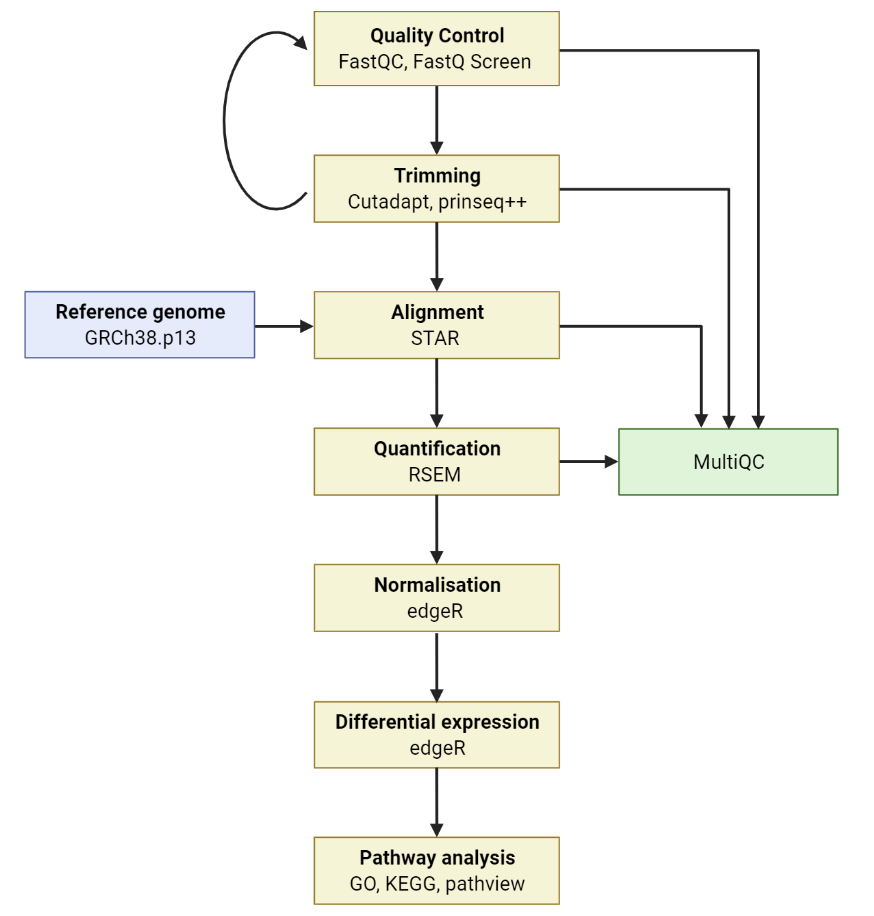
\includegraphics[width=1\textwidth]{Dissertation_pipeline}
    \caption[General overview of the RNA-seq pipeline.]{General overview of the RNA-seq pipeline. Created with \href{https://biorender.com/}{BioRender.com}.} 
    \label{fig:Dissertation_pipeline}
\end{figure}

\clearpage
%%%%%%%%%%%%%%%%%%%%%%%%%%%%%%%%%%%%%%%%%%%%%%%%%%%%%%%%%%%%%%
\subsection{Quality Control}%%%%%%%%%%%%%%%%%%%%%%%%%%%%%%%%%%%%%%%%%%%%%
%%%%%%%%%%%%%%%%%%%%%%%%%%%%%%%%%%%%%%%%%%%%%%%%%%%%%%%%%%%%%%
% Maybe list used arguments and their use like evas documentation??

The first step of any sequencing pipeline should be the assessment of the quality of the raw data files. Sequencing information of poor quality is identified if present, and if necessary, truncated to mitigate inaccuracies in the downstream pipeline. To assess the quality of the FASTQ files, they were ported to FastQC v0.11.9 \citep{andrews2010fastqc} using eight threads (\autoref{lst:FastQC}). This extracted information on the sequences, including Phred scores, GC content, N content, sequence length distribution, sequence duplication levels, overrepresented sequences and adapter sequences. FastQC rates each of these modules using a green check-mark signifying that it 'passed' QC, a yellow exclamation mark 'warning', or a red cross 'failed'. 

Two modules failed consistently throughout the four samples received: 'Sequence Duplication Levels' and 'Per base sequence content'. This is normal and expected for RNA data, and is explained in further detail in \autoref{Assessing the Quality of the Raw FASTQ files}. Traces (<0.5\%) of TruSeq adapters were detected in the FASTQ files, which is corroborated by the sequencer's manual \citep{HiSeq2000} stating that it makes use of the 'TruSeq family of reagents'. 

\begin{lstlisting}[language=bash, caption=FastQC command, label={lst:FastQC}]
# FastQC accepts multiple input files, so we can use wildcards
fastqc \
 -t 8 \
 -o ./raw_FastQC_out \
*.fq 
\end{lstlisting}

Next, Fastq Screen v0.14.0 \citep{wingett2018fastq} was used to check for RNA contaminants from other common sources, by comparing the reads against a set of sequence databases (\autoref{lst:FastqScreen}). Perl, an aligner (Bowtie \citep{bowtie}, Bowtie2 \citep{bowtie2} or BWA \citep{bwa}) and a Linux-based operating system are required. Bowtie2 was used to align the sample reads to the reads in the contaminant database.

\begin{lstlisting}[language=bash, caption=FastqScreen command, label={lst:FastqScreen}]
# FastQScreen also accepts multiple file inputs
fastq_screen \
--aligner bowtie2 \
--conf ./fastq_screen.conf \
 *.fq 
\end{lstlisting}


%%%%%%%%%%%%%%%%%%%%%%%%%%%%%%%%%%%%%%%%%%%%%%%%%%%%%%%%%%%%%%
\subsection{Preprocessing}%%%%%%%%%%%%%%%%%%%%%%%%%%%%%%%%%%%%%%%%%%%%%%
%%%%%%%%%%%%%%%%%%%%%%%%%%%%%%%%%%%%%%%%%%%%%%%%%%%%%%%%%%%%%%
Poor quality reads lead to poor downstream sequence analysis. Thus, it is common practice in RNA-seq to trim the undesired regions. Cutadapt \citep{martin2011cutadapt} was used to trim the previously detected TruSeq adapter sequences and short reads, using a threshold of <45 bp. Between 1.3 and 1.6\% of the base-pairs were trimmed across the four samples. Cutadapt was accessed through the wrapper script Trim Galore! v0.6.7 \citep{trimgalore} which instantly redirects the trimmed data back to FastQC to assess the improvement in quality, if any.

\begin{lstlisting}[caption=Trim Galore! trimming]
trim_galore \
--phred33 \
--fastqc \
-a "GATCGGAAGAGCACACGTCTGAACTCCAGTCAC" \
--length 45 \
-o trim_galore_output \
--fastqc_args "-o trimmed_FastQC_out -t 8" \
--cores 4 \
*.fq 
\end{lstlisting}

The trimmed files were further filtered using Prinseq++ \citep{prinseq++} which removed ambiguous reads containing >7 N's and sequences with a DUST score\footnote{A value between 0 and 1 generated by the DUST algorithm which is a measure of sequence complexity. Here, its purpose is to mask low-complexity regions.} of <0.1.

\begin{lstlisting}[caption=Prinseq++ filtering]
samples=(control, 1hour, 6hour, 12hour)
mkdir prinseq_out

for sample in ${samples[@]};
do
        prinseq++ \
        -fastq ./trim_galore_output/${sample}_trimmed.fq \
        -out_name ./prinseq_out/${sample}_filtered.fq \
        -out_bad ./prinseq_out/${sample}_bad.fq \
        -ns_max_n 7 \
        -lc_dust=0.1 > ./prinseq_out/control_prinseq_report.txt
done
\end{lstlisting}

\subsection{Read alignment and Quantification}
The trimmed and filtered FASTQ files were aligned to the GRCh38.p13 reference genome \citep{ref} using the \ac{STAR} 2.7.9a aligner \citep{Dobin2013}. \ac{STAR} was called through RSEM v1.3.3 \citep{li2011rsem}, which after alignment estimates gene and isoform expression levels. RSEM must be accessed through a 64 bit Linux or Mac OS command-line, and must have C++, Perl and R installed as dependencies.

Reference transcripts from the reference genome were first generated through the \texttt{rsem-prepare-reference} program, with the help of its respective GTF file (\autoref{lst:RSEM_ref}). 

% .genes.results (one row per gene) which has the headers: gene_id transcript_id(s)        length  effective_length        expected_count  TPM     FPKM
% .isoforms.results (one row per transcript) which has the headers: transcript_id   gene_id length  effective_length        expected_count  TPM     FPKM    IsoPct

\begin{lstlisting}[caption= reference generation, label={lst:RSEM_ref}]
mkdir RSEM
mkdir RSEM/reference
rsem-prepare-reference --gtf mm9.gtf \
                       --star \
                       --star-sjdboverhang 50 \
                       --num-threads 8 \
                       --gtf Homo_sapiens.GRCh38.104.gtf \
                       Homo_sapiens.GRCh38.dna.primary_assembly.fa \
                       ./RSEM/reference/GRCh38
\end{lstlisting}

The \texttt{--star-sjdboverhang} is an argument passed to \ac{STAR} which sets the maximum possible overhang for the reads. It should be equal to the read length minus one. In our case, the read length is 51, thus a value of 50 is used. The final variable is a prefix to the output files. This may be used as the output path for the generated reference files.

To calculate expression values, the \texttt{rsem-calculate-expression} command is used. As before, the final argument is a prefix to the output files, and the argument before that is the path to the reference files created in the previous command. RSEM first uses \ac{STAR} to align the filtered sample reads to the generated reference reads, creating a BAM file sorted by its coordinates. It outputs two quantification files per sample, with differing suffices: one ending in '.genes.results' and another '.isoform.results'. These are both tab-delimited text files with similar headers, with the former dedicating a row for each gene and the latter dedicating a row for each transcript. The isoform-centric file thus contains more data, which are unnecessary for our objectives. Of the columns in the gene-centric file, two will be used in the subsequent step: 'gene\textunderscore id' which holds the Ensembl gene ID, and 'TPM' which holds the normalised read count for the respective gene.

\begin{lstlisting}[caption=RSEM expression command, label={lst:RSEM_exp}]
mkdir RSEM/expression
samples=(control, 1hour, 6hour, 12hour)

for sample in ${samples[@]};
do
        rsem-calculate-expression \
        --num-threads 16 \
        --star \
        --sort-bam-by-coordinate \
        ./prinseq_out/${sample}*good_out.fq \
        ./RSEM/reference/GRCh38 \
        ./RSEM/expression/${sample}
done
\end{lstlisting}

\subsection{Reassessing the Quality}

The produced files from FastQC, FastQScreen, Trim Galore! and RSEM, were funnelled into MultiQC v1.11 \citep{multiqc} which summarises their output in the form of an HTML report. At the time of writing, the latest version of MultiQC did not support Prinseq++ and its log files were inspected manually instead.

\begin{lstlisting}[language=bash, caption=MultiQC command]
multiqc \
-o ./multiqc_out \
./trim_galore_output/*txt \
./fastqc/FastQC_out/. \
./FastQ_Screen_out/raw/. \
./RSEM/expression/.
\end{lstlisting}

\subsection{Normalisation and Differential Gene Expression}
% Find another name for this?

We have chosen edgeR v3.14 \citep{edger} as the package to help identify differentially expressed genes, which supports datasets that lack replicates such as our own. The instructions on the vignette\footnote{\url{https://www.bioconductor.org/packages/release/bioc/vignettes/edgeR/inst/doc/edgeRUsersGuide.pdf}} were followed, and are summarised as follows. 

The four gene read count files generated through RSEM were imported into the R script v3.6.3 \citep{R} and had their gene IDs (1st column) and expected read counts (5th column) compiled into a single \texttt{DGEList} object which consists of multiple data-frames. 

\begin{lstlisting}[language=R, caption=Importing count files to R]
files <- list("1hour.genes.results", "12hour.genes.results", 
"6hour.genes.results", "control.genes.results")
path <- "/path/to/files/"
labels = c('1hr', '12hr', '6hr', '0hr')
group <- factor(labels)
y <- readDGE(files, path=path, columns=c(1,5), group=group, labels=labels)
\end{lstlisting}

\subsubsection{Filtering Low Count Genes}

Genes with low counts (<10) are generally considered as noise, as they are not expressed at any biologically meaningful level and filtering them would reduce the amount of statistical tests required in the downstream analysis \citep{law2016rna}. EdgeR provides the function \texttt{filterByExpr} which serves this purpose.

\begin{lstlisting}[language=R, caption=Filtering low count genes]
library(edgeR)
keep <- filterByExpr(y, group=group)
table(keep)  # How many genes were removed and how many remain
y <- y[keep,keep.lib.sizes=FALSE]
\end{lstlisting}

\subsubsection{Gene Annotation}

The remaining genes were annotated using the AnnotationDbi library v3.14 \citep{annotationdbi} which is dependent on the org.Hs.eg.db v3.10.0 \citep{org.Hs.eg.db} human annotation database. These were used to add the Entrez ID annotation to the \texttt{DGEList} object, which will be used for pathway analysis further downstream. AnnotationDbi provides other useful annotation options, but were excluded as  combination of annotations was causing a one to many mapping error. This step was later repeated (after pathway analysis) to add gene symbol annotations. This proved useful for later research into their biology, since most papers refer to the gene by its gene symbol.

\begin{lstlisting}[language=R, caption=Annotation step]
library(org.Hs.eg.db)
library(AnnotationDbi) 

# This step was repeated at a later stage with "SYMBOL" as the
# column argument, which adds the gene symbol.
Symbol <- mapIds(org.Hs.eg.db, keys=rownames(y), keytype="ENSEMBL",
                 column="ENTREZID")

y$genes <- data.frame(Symbol=Symbol)
head(y$genes)
\end{lstlisting}

\subsubsection{Normalisation}

The read counts are then normalised by the \texttt{calcNormFactors} function which uses the \ac{TMM} method. This is recommended by the edgeR vignette and is explained in detail in \cite{robinson2010scaling}. The aim of normalisation is to mitigate any technical bias on the data.
% Maybe write more here

\begin{lstlisting}[language=R, caption=TMM normalisation]
y <- calcNormFactors(y)
design <- model.matrix(~group)
\end{lstlisting}

EdgeR has multiple methods to determine which genes are differentially expressed, but the classic \texttt{exactTest} was deemed as most appropriate. This is a pairwise test which compares the means between two groups of counts with a negative-binomial distribution. The calculation of the dispersion of our data is required prior to its use, however this is not mathematically possible due to our lack of replicates. In such cases the edgeR vignette suggests that estimating the dispersion based on the experimental conditions is more scientifically sound than assuming no variation. It should be emphasised that this technique is inaccurate, but was deemed as the best possible option for statistical analysis without replicates (further detail in Section \ref{Adapting Differential Gene Expression Analysis to a Lack of Replicates}).

The \ac{BCV} is equal to the square root of the dispersion, and the vignette suggests a few estimates for the \ac{BCV}, such as '0.1 for data on genetically identical model organisms'. While this is human data, not a model organism, the data originate from the same genetically identical cell line, and this value was deemed appropriate. Thus the dispersion used for \texttt{exactTest} is equal to the BCV\textsuperscript{2}, or 0.01. 
The test was performed a total of three times, where each treated sample was compared with the control. This returns a \texttt{DGEExact} object for each comparison, containing the $log_{2}$ fold change (logFC), $log_{2}$ Counts Per Million (logCPM), p-values and annotations for each gene. 

\begin{lstlisting}[language=R, caption=Exact test function]
bcv <- 0.1
et_12 <- exactTest(y, pair=c(1, 2), dispersion=bcv^2)
et_1 <- exactTest(y, pair=c(1, 3), dispersion=bcv^2)
et_6 <- exactTest(y, pair=c(1, 4), dispersion=bcv^2)
\end{lstlisting}

% EdgeR has three ways of judging differential expression but exactTest was deemed as the best fit

\subsubsection{Adjusting p-values and Cut-offs}

Multiple testing is an inherent risk of RNA-seq due to its vast amounts of comparisons and adjusting p-values is a common technique implemented into the RNAseq pipeline to help compensate for this.  The \ac{FDR} with the Benjamini-Hochberg controlling procedure was the chosen p-value adjustment method. This produced value is the proportion of false positives one might expect to get from a test. Each of the \texttt{DGEExact} objects was transformed in this way using the \texttt{topTags} function. Differential expression was sorted by the \ac{FDR} and any genes with an \ac{FDR} < 0.05 were filtered out, which means that we are willing to accept that 5\% of all \ac{DEG} will be false positives. Filtering on the logFC was then performed manually, using a threshold of 1.5.  

%Summary of  https://www.science.smith.edu/cmbs/wp-content/uploads/sites/36/2015/09/P-and-q-values-in-RNA-Seq.pdf:
%		FDR makes use of Q-values which usually result in a smaller number of false positives, although this is not always the case:
%		An FDR-adjusted p-value (aka a q-value) of 0.05 implies that we are willing to accept that 5% of the tests found to be statistically significant (e.g. by p-value) will be false positives

%'Many traditional techniques such as the Bonferroni correction are too conservative in the sense that while they reduce the number of false positives, they also reduce the number of true discoveries.': https://www.nonlinear.com/support/progenesis/comet/faq/v2.0/pq-values.aspx

\begin{lstlisting}[language=R, caption=Adjusting p-values and filtering data based on the logFC and FDR]
FDR_thresh <- 0.05  # removes rows with FDR less than this
et_1_toptags <- topTags(et_1, n=nrow(et_1$table), adjust.method="BH", 
sort.by="PValue", p.value=FDR_thresh)$table
et_12_toptags <- topTags(et_12, n=nrow(et_12$table), adjust.method="BH", 
sort.by="PValue", p.value=FDR_thresh)$table
et_6_toptags <- topTags(et_6, n=nrow(et_6$table), adjust.method="BH", 
sort.by="PValue", p.value=FDR_thresh)$table

FC_thresh <- 1.5  # removes rows with a logFC less than this
et_1_toptags <- et_1_toptags[abs(et_1_toptags$logFC) > FC_thresh, ]
et_12_toptags <- et_12_toptags[abs(et_12_toptags$logFC) > FC_thresh, ]
et_6_toptags <- et_6_toptags[abs(et_6_toptags$logFC) > FC_thresh, ]
\end{lstlisting}

\subsection{Functional analysis}
?

% The main components of an DGEList object are a matrix counts containing the integer counts,
% a data.frame samples containing information about the samples or libraries, and a optional
% data.frame genes containing annotation for the genes or genomic features


%EdgeR manual:
%A commonly used approach is to conduct DE tests, apply a fold-change cut-off and then rank all the genes above that fold-change threshold by p-value. In some other cases genes are first chosen according to a p-value cut-off and then sorted by their fold-changes.

%\subsubsection{Gene Set Enrichment Analysis and Pathway Analysis}
%\ac{GO}
%\ac{KEGG}
% https://www.biostars.org/p/462980/
% pathways
% library(pathview)
% HOUSEKEEPING GENES for sanity checks 
%https://www.genomics-online.com/resources/16/5049/housekeeping-genes/

\section{Summary}
Empty for now.

    \chapter{Results \& Discussion}

In this chapter we will present and discuss the relevant outputs of our RNA-seq pipeline, and the reasoning behind our chosen approach, with accordance to the project's aim and objectives (\autoref{Aim and Objectives}). As described thoroughly in \autoref{pipeline}, we have:

\begin{itemize}
\item Performed QC checks on the four raw FASTQ files, and filtered out data with signs of poor quality.
\item Aligned the reads to the GRCh38.p13 reference genome, excluding reads with ambiguous mapping, to produce gene-centric read count matrices.
\item Filtered genes with low counts (<10), as these would be indistinguishable from noise.
\item Normalised the read counts for biologically irrelevant extraneous variables between the libraries using the \ac{TMM} method.
\item Quantified the magnitude and significance of the differences in gene expression between the treated samples and the control. These were represented as the \ac{logFC} and \textit{p}-values respectively, given for each gene and stored in a data frame.
\item Adjusted the \textit{p}-values for multiple-testing, converting them to \ac{FDR}s with the Benjamini-Hochberg controlling procedure.
\item Set an \ac{FDR} cut-off of 0.05 and a \ac{logFC} cut-off of 1.5 to define which genes are truly differentially expressed.
\item Annotated the \ac{DEG}s and performed Gene Set Enrichment Analysis to put them into their biological context.
\end{itemize}


\section{Determining the Optimal Tools}
\label{determining tools}

Before we begin tackling the pipeline, we should first explain the reasoning behind the choices of its constituent tools. This will make heavy use of the literature reviewed in Section \ref{Computational Tools}, through which we will achieve this project's first objective. Extensive descriptions of the final tools implemented in the pipeline can be found throughout Section \ref{RNA-seq: in silico}.
% NOTE SEE IF U NEED TO CHANGE THIS. Maybe group all the tools in a single place

Tools which measure quality metrics without altering the data require little justification for their use, their mention occasionally being completely omitted from RNA-seq studies (\autoref{tab:rnaseq_experiments}). \textbf{FastQC} provides a detailed analysis of the contents of FASTQ files and highlights indications of low quality reads. While FastQC results are detailed, they lack the detection of external nucleotide contaminants in the data. This information was supplemented with the results from \textbf{FastQScreen} which aligns the experimental sequences to common contaminant sequences (e.g. mouse, \textit{Drosophila}, rRNA) and provides a graph marking any successful alignments. \textbf{MultiQC} is a staple of sequencing data quality control, unparalleled in its ability to combine logs from a wide range of supported tools and across multiple samples. This greatly facilitates cross-sample comparisons.

\cite{he2020assessing} found that the effects of their tested preprocessing techniques on downstream analyses are marginal, thus we base our decision on the frequency of the tools used in tables \ref{tab:rnaseq_experiments} and \ref{tab:packaged_pipelines} and their functionality. \textbf{Cutadapt} adequately satisfies these criteria, providing the means to trim adapter sequences and remove short reads. \textbf{Trim Galore!} pipes the output to FastQC, which facilitates the reassessment of quality. To complement their functionality, \textbf{Prinseq++} was chosen to detect and remove regions of low-complexity which were noticeably neglected in studies' preprocessing steps. 
%\cite{liao2020read} and \cite{he2020assessing} doubt the necessity of trimming at all.

Despite \textbf{STAR} being demanding of RAM \citep{Dobin2013} and slower than more light-weight aligners \citep{srivastava2020alignment}, these were not limiting factors due to our access to a High Performance Computer (HPC) and small number of samples. \cite{srivastava2020alignment} found that the choice between quasi-mappers (e.g. Salmon) and traditional aligners (e.g. STAR) is a trade-off between speed and accuracy. Similarly \cite{Zhang2017} found that pseudo-aligners Salmon and Kallisto require less runtime while maintaining similar accuracy to STAR. \cite{Schaarschmidt2020} find that the effect aligners have on the final list of \ac{DEG}s is negligible, and that all tested aligners can be used equally for RNA-seq. Even if STAR provides even a marginal increase in accuracy over quasi-aligners, this is preferable over any improvements in speed or computational demand provided by other aligners.

An RNA-seq quantification tool benchmark, \cite{teng2016benchmark}, conclude that their tested tools performed similarly, with the exception of the under-performing Flux Capacitor \citep{} and eXpress \citep{}. \textbf{RSEM} was amongst these tools, and was ultimately chosen on the basis of its statistical techniques based on \cite{li2010rna} to mitigate ambiguous read alignment. Its support for the STAR aligner is also convenient, allowing the combination of alignment and quantification steps. 

The choice of tools for downstream analyses was more complex, and deservent of their own subsections as follows.


\subsection{Adapting DGE Analysis to a Lack of Replicates}
\label{DGE no replicates}

The most difficult and time-consuming decision to make was the choice of tool to perform \ac{DGE} analysis. The invested effort was justified by the findings of \cite{williams2017empirical}, which state that the method of \ac{DGE} exhibits the strongest impact on the results out of all stages of the pipeline. Our data consists of three time points (1hr, 6hr, 12hr) and a negative control, each lacking replicates. 

Technical replicates allow the isolation of the non-biological variation to evaluate the quality of the instruments and methodology used. By contrast, biological replicates originate from different biological sources and are meant to test the biological variance of the samples. \cite{liu2014rna} find that in RNAseq biological variation is by far more important, and given a choice between the two, the researcher should invest in biological replicates. \cite{bullard2010evaluation} confirm this claim, finding that technical variation in RNAseq experiments is minimal. \cite{schurch2016many} found that using three biological replicates gave 20\% to 40\% of the \ac{DEG}s (varies according to the tool) compared to a full set of 42 replicates (representing the 'true' population). This rises to >85\% when considering genes with a log$_2$ fold change of >2. \cite{schurch2016many} state that ideally an RNAseq experiment for \ac{DGE} should have a minimum of six replicates per condition for all experiments and 12 replicates for experiments where the identification of \textit{all} the \ac{DEG}s, even the lowly expressed ones, is important. 

However, in practice, performing an experiment with large numbers of replicates is not always possible. Budget constraints and the still-high cost of sequencing are a common issue in RNAseq experiments. One may argue that this issue is mitigated due to the negligible technical variance of RNA-seq \citep{bullard2010evaluation} and the minimal biological variance in samples from the same \ac{ATRA}-resistant HL-60 cell line. In spite of this, the statistical tests used by conventional \ac{DGE} tools are dependent on the calculation of the variance or dispersion, which is not mathematically possible with a single reading per condition. To make the most of such datasets, several \ac{DGE} tools advertise their ability to work with just a single reading per experimental condition \citep{feng2012gfold, gim2016lpeseq, anders2010differential, wang2010degseq, al2014bootstrap}. Notably, DESeq2 does not support datasets without replicates. There is an unfortunate lack of review papers and independent studies which benchmark these tools. For this reason this section will be reviewing the available tools adapted to performing \ac{DGE} without replicates.

The first tool in this review will be \textbf{GFOLD} \citep{feng2012gfold}, developed specifically for datasets lacking in replicates. The developers acknowledge the dependence of \textit{p}-values on variance estimation, which is impossible without replicates. A unique GFOLD value replaces the standard metrics of significance (\textit{p}-values) and expression change (log$_2$ fold changes). \cite{feng2012gfold} describe the value as a relative change of the expression level. GFOLD is unique in that it is the only tool in this comparison that is called through the Linux command line, instead of being an R library.

\textbf{LPESeq} \citep{gim2016lpeseq} introduces the Local-Pooled-Error (LPE) method for few or single-replicate \ac{DGE} analysis. This method attempts to estimate transcript-specific variance using the raw values of each transcript per condition. Hypothesis testing for significant difference is then performed to identify the differentially expressed genes.

\textbf{IsoDE} \citep{al2014bootstrap} is a non-parametric method (i.e. it assumes no statistical distribution) and is based on bootstrapping. The algorithm generates FPKM estimates from read counts of each condition which undergo pairwise comparison.

An MA-plot-based method, the R library \textbf{DEGseq} \citep{wang2010degseq} (not to be confused with DESeq) accepts input .bed or .eland input files and outputs an XHTML page with \textit{p}-values, gene expression values and expression differences in the form of Q-values.

The final tool in this review is the Bioconductor R library \textbf{edgeR} \citep{edger}. It may be more accurately described as a collection of methods, neither of which are specifically adapted to data without replicates, but its documentation provides recommendations to adapt the analysis to such a situation. EdgeR and its normalisation technique TMM have already been covered extensively in Section \ref{EdgeR} and Section \ref{TMM} respectively. 

The lesser-known tools (GFOLD, LPESeq, DEGseq, IsoDE), while developed specifically to function without replicates, were found to be limited in functionality in comparison to \textbf{edgeR}. Additionally, due to their rather unconventional approach to \ac{DGE}, their output was found to be incompatible with other downstream libraries, limiting the potential for data exploration. 

EdgeR has multiple methods to determine which genes are differentially expressed (\autoref{edger_dge_options}). The likelihood ratio tests \citep{mccarthy2012differential} compared values against their mean, which was not applicable to our study as we needed to compare reads from treated cells against reads from untreated cells. Quasi-likelihood F-tests \citep{lun2016s, lund2012detecting} were simply not compatible to datasets lacking replicates. This leaves us with the \textit{classic} approach: the exact test for the negative binomial distribution \citep{robinson2007moderated, robinson2008small}. This is a pairwise test which compares the means between two groups of counts, applicable to experiments with a single factor. It should not be confused with Fisher's exact test \citep{fisher1922interpretation}, although the two share a number of similarities \citep{chen2014edger}.

The exact test for the negative binomial distribution still involves the calculation of dispersion of the data, but the edgeR vignette suggests a method to circumvent this. It suggests nominal values for the biological variation (\ac{BCV}) of our data based on previous experiments, from which we may derive an estimation for the dispersion. The vignette emphasises that this method is still inaccurate, but was deemed as the best possible solution given our data and the aforementioned potential techniques. By extension, the normalisation method native to edgeR, \textbf{TMM}, will be used to ensure proper function of the library.
% really perfect paper https://www.ncbi.nlm.nih.gov/pmc/articles/PMC4878611/#:~:text=Recommendations%20for%20RNA%2Dseq%20experiment%20design&text=At%20least%20six%20replicates%20per,all%20DE%20genes%20is%20important.

\subsection{Gene Set Analyses}

For further analyses on a gene-set level (e.g. involving \ac{GO} terms or \ac{KEGG} pathways), we must consider three main approaches described by \cite{khatri2012ten} and \cite{alhamdoosh2017combining}, ranked in order of increasing complexity: Over-Representation Analysis (\ac{ORA}), Gene Set Enrichment Analysis (\ac{GSEA}) and Pathway Topology Analysis (\ac{PTA}). More complex analyses with more factors implies greater accuracy, and \cite{nguyen2019identifying} confirms this intuition, showing that \ac{PTA} methods perform the best as they take into account the interactions between gene products, and the nature of their interaction (e.g. activation or inhibition). Conversely, the more complex the process, the harder it is for researchers to truly understand the underlying mechanisms and risk applying them incorrectly. A presentation by Pietrosemoli and Legendre\footnote{\url{https://ressources.france-bioinformatique.fr/sites/default/files/4\%20-\%20FGSA_Roscoff.pdf} (Last accessed 07/07/22)} references the principal of Occam’s Razor, which states that solutions should not be complicated beyond necessity. \cite{albert2020biostar} agrees that rather than believing that a 'black box' will work as one would wish, the researcher might prefer to use slightly simpler but comprehensible techniques.

For this project, \ac{GSEA} tools were chosen as a compromise between risk of human error and statistical accuracy, as a balance between these two philosophies. For this project we have chosen \textbf{GAGE} as the specific library that will generate the gene-set-level statistics to check which gene sets are differentially expressed. EdgeR has its own inbuilt gene set analysing functions, \texttt{goana} and \texttt{kegga}, however these only test for over-representation. This means that the analysis excludes important factors such as \ac{logFC}s and \textit{p}-values, and fails to output the direction of regulation of the gene set.
%Pathview?

\section{Read Quality Control}

This section encompasses all QC measures taken prior to quantification of the reads. MultiQC is able to read and compile log files from FastQC, FastQScreen, Cutadapt and STAR into a single interactive HTML file, allowing quality comparisons across samples. Figures \ref{fig:fastqc-status-check-heatmap} through \ref{fig:star_alignment_plot} are graphs downloaded directly from MultiQC.


\subsection{Assessing the Quality of the Raw Data}
\label{Assessing the Quality of the Raw Data}
We started off with four single-ended 50bp FASTQ files, one per experimental time point (control, 1hr, 6hr, 12hr), which were sequenced using the Illumina Stranded mRNA-seq workflow \citep{HiSeq2000}. Paired-end reads of a longer length would have been more accurate, although on their website\footnote{\url{https://emea.illumina.com/science/technology/next-generation-sequencing/plan-experiments/read-length.html} (Last accessed 16/06/22)}, Illumina suggests that single-ended 50bp reads suffice for a \ac{DGE} RNA-seq experiment.

\autoref{fig:fastqc-status-check-heatmap} shows the FastQC results for each raw file, summarised as a heatmap generated by MultiQC. Caution should be exercised when interpreting RNA data through FastQC, as the program is primarily calibrated to DNA data. Two modules failed consistently throughout the four samples received. This is normal and expected even for high-quality RNA \citep{hansen2010biases}. The failure of the \textit{Per base sequence content} module can be explained by a benign artefact of the random hexamer priming that occurs during library preparation, where the first 10-15 bases of RNA reads are non-uniformly enriched \citep{hansen2010biases}. The failure for the second module, textit{Sequence Duplication Levels} is explained by \autoref{fig:fastqc_sequence_duplication_levels_plot} and the text preceding it.

All four samples had <0.3\% \textit{N}-content on average on the first base of the reads and <0.1\% on the rest of the read, which the algorithm deems as good quality. All sequences of all samples had a single length of 51bp with <1\% overrepresented sequences and <0.5\% adapter contamination.

%Write about terminator caps in intro

% https://hbctraining.github.io/Intro-to-rnaseq-hpc-salmon/lessons/qc_fastqc_assessment.html
% Really good resource on RNAseq QC
 %Another one: https://rtsf.natsci.msu.edu/genomics/tech-notes/fastqc-tutorial-and-faq/#:~:text=FastQC%2C%20written%20by%20Simon%20Andrews,on%20a%20sequence%20data%20set.


% INTERNPRETING FASTQC REPORT NOTES:
% Real good resource of possible explanations:
% We have positional sequence bias: https://sequencing.qcfail.com/articles/positional-sequence-bias-in-random-primed-libraries/
% High Sequence Duplication levels are expected: https://www.biostars.org/p/307361/
%From Molecular Biology assignment:
%  One cycle per base pair would have been needed, so 50 cycles should have been performed.


\newpage
\begin{figure}[!h]
    \centering
    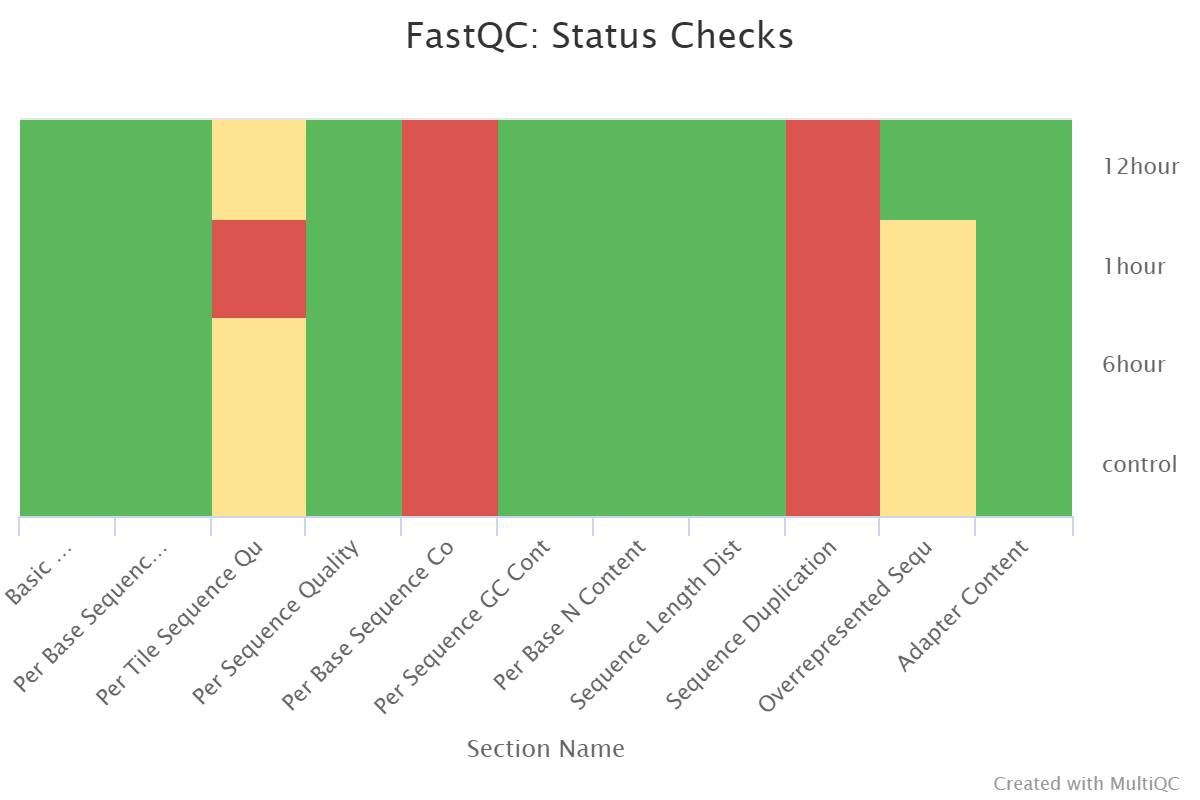
\includegraphics[width=1\textwidth]{fastqc-status-check-heatmap}
    \caption[Heat map showing the status of each FastQC module]{Heat map generated by MultiQC showing the status of each FastQC module: Pass, Warning or Fail.} 
    \label{fig:fastqc-status-check-heatmap}
\end{figure}

\newpage
Part of the sequencing process involved PCR amplification of cDNA, although not all sequences are amplified equally \citep{kozarewa2009amplification}. These PCR duplicates differ from 'natural' duplicates, i.e. those that originated from different mRNA molecules. Both these factors contribute to certain sequences being disproportionately abundant (as seen in \autoref{fig:fastqc_sequence_duplication_levels_plot}), which FastQC flags as duplicates, causing the failure of the \textit{Sequence Duplication Levels} module. \cite{parekh2016impact} state that there is no clear consensus on what should be done with these duplicates, with their removal producing conflicting results.

\begin{figure}[!h]
    \centering
    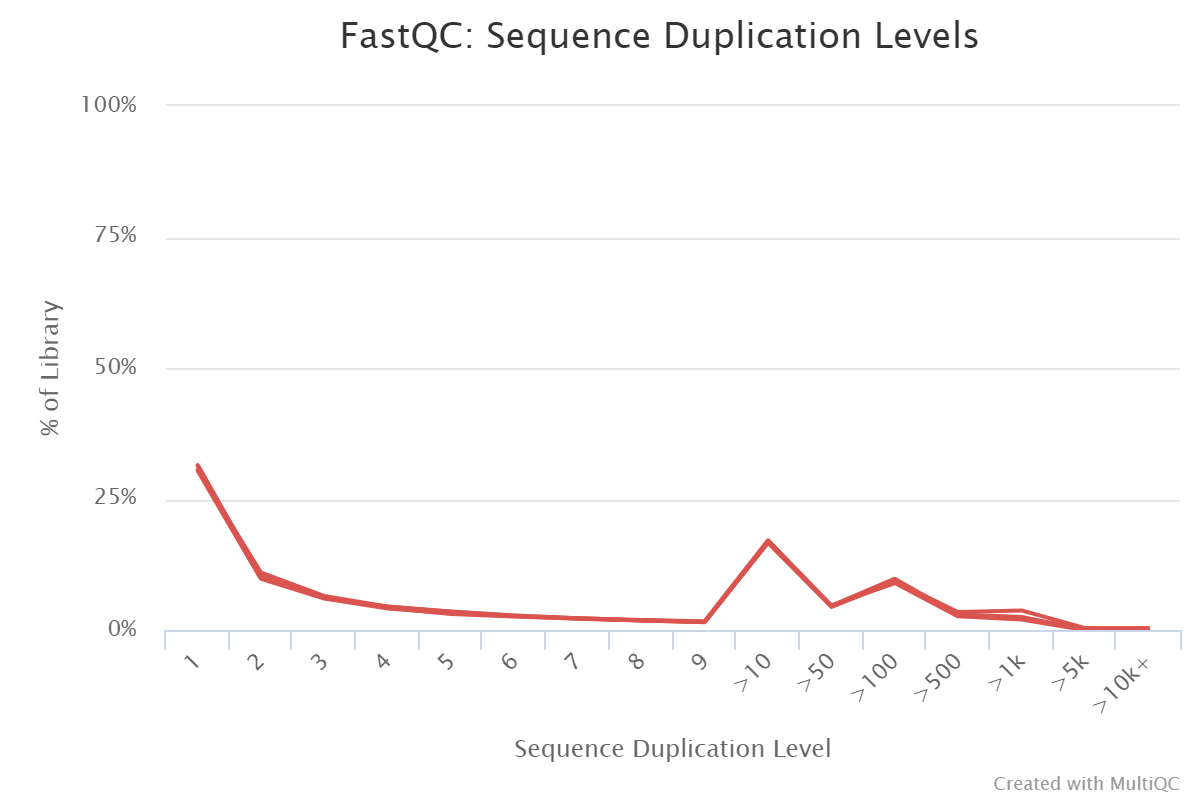
\includegraphics[width=1\textwidth]{fastqc_sequence_duplication_levels_plot}
    \caption[Sequence duplication levels plots for all samples]{Sequence duplication levels plots for all samples, showing the wide range of possible coverages in RNA data, ranging from 1 to >10,000.} 
    \label{fig:fastqc_sequence_duplication_levels_plot}
\end{figure}

\newpage
In Figure \ref{fig:fastqc_per_base_sequence_quality_plot}, sequence quality peaks at around the 14th base-pair, then gradually declines which is a classic sign of phasing. \cite{pfeiffer2018systematic} describe it as two similar phenomena: pre-phasing and post-phasing, both of which cause the reads to become out-of-sync. Pre-phasing occurs when two or more nucleotides bind to the read in a single cycle, causing the sequence to ‘skip’ a nucleotide. This often occurs when the flow-cell is not flushed properly or in the case of a defect terminator cap. Post-phasing is caused by the incomplete removal of the terminator cap, leading to the sequence lagging behind the rest of the cluster. As the number of cycles increases, the higher the probability of an error to occur which causes the read to become out of phase, and when this occurs, it will pollute the light signals of all subsequent cycles.


\begin{figure}[!h]
    \centering
    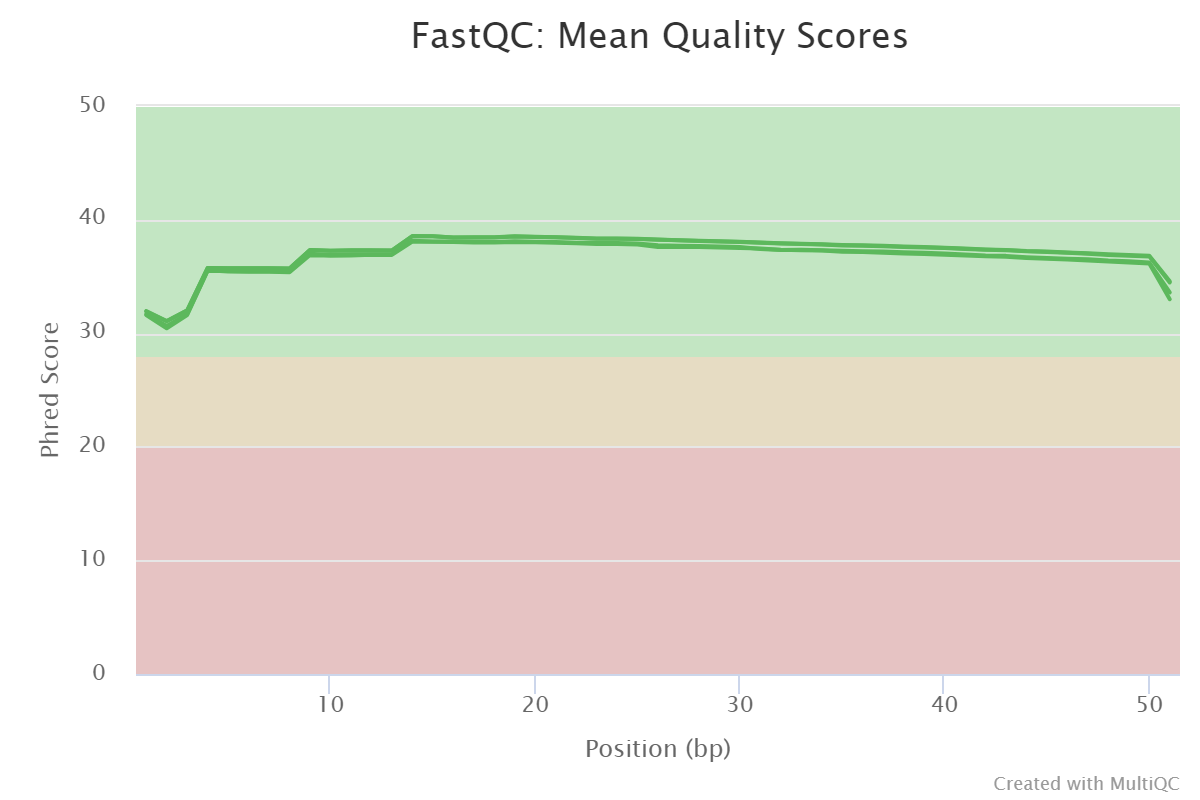
\includegraphics[width=1\textwidth]{fastqc_per_base_sequence_quality_plot}
    \caption{The aggregated mean Phred scores at each position of the reads.} % write about tpical pattern
    \label{fig:fastqc_per_base_sequence_quality_plot}
\end{figure}

\newpage
\autoref{fig:fastqc_per_sequence_gc_content_plot} shows a normal distribution which peaks around 48 \%GC, which is within the expected range for a human genome \citep{meunier2004recombination}. During PCR, endonucleases are less likely to cleave GC base pairs for two reasons: their triple bond, which is stronger than the double bond in AT pairs, and because of  a phenomenon called base stacking which contributes to its structural stability \citep{yakovchuk2006base}. This may lead to GC-bias \citep{benjamini2012summarizing}, although this does not seem to be present.

\begin{figure}[!h]
    \centering
    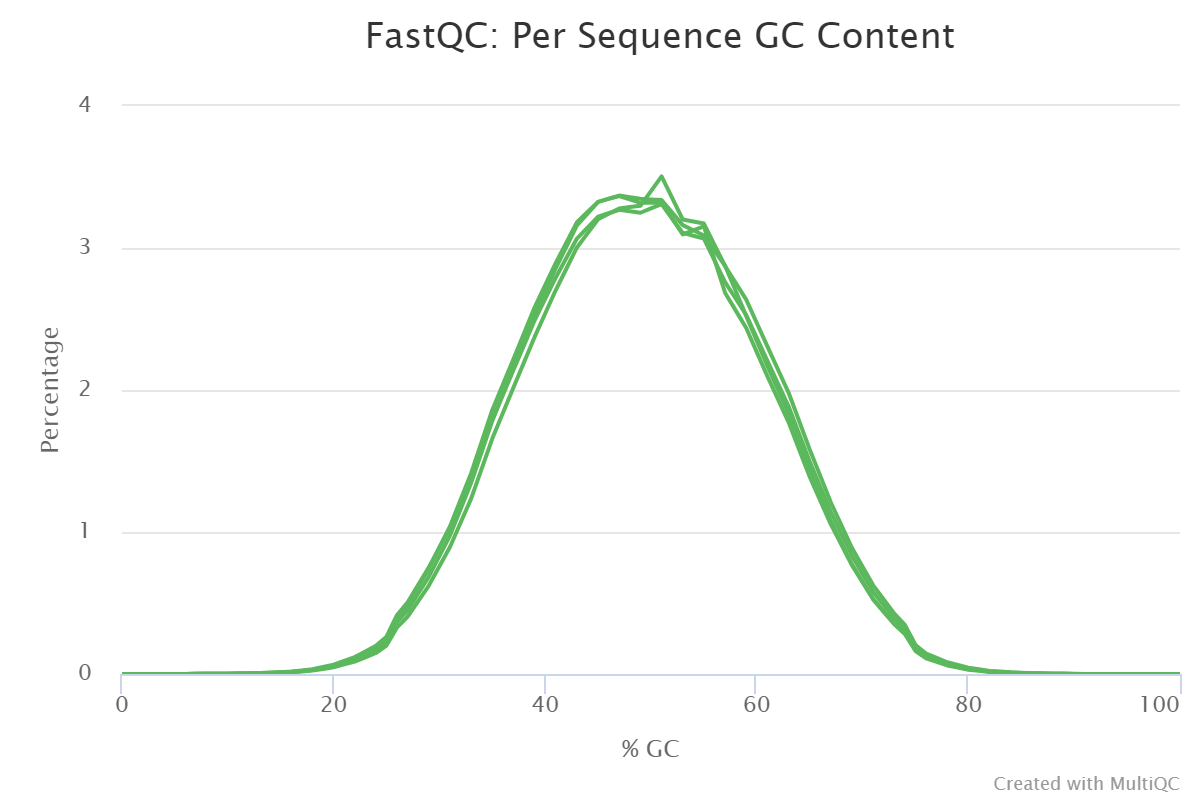
\includegraphics[width=1\textwidth]{fastqc_per_sequence_gc_content_plot}
    \caption{The distribution of GC percentages across the reads.}
    \label{fig:fastqc_per_sequence_gc_content_plot}
\end{figure}

\newpage
\autoref{fig:fastqc_per_sequence_quality_scores_plot} is similar to  \autoref{fig:fastqc_per_base_sequence_quality_plot}, except showing \textit{average} Phred scores on a sequence-level, instead of a base pair-level. The Phred score distribution is as expected for good quality data.


\begin{figure}[!h]
    \centering
    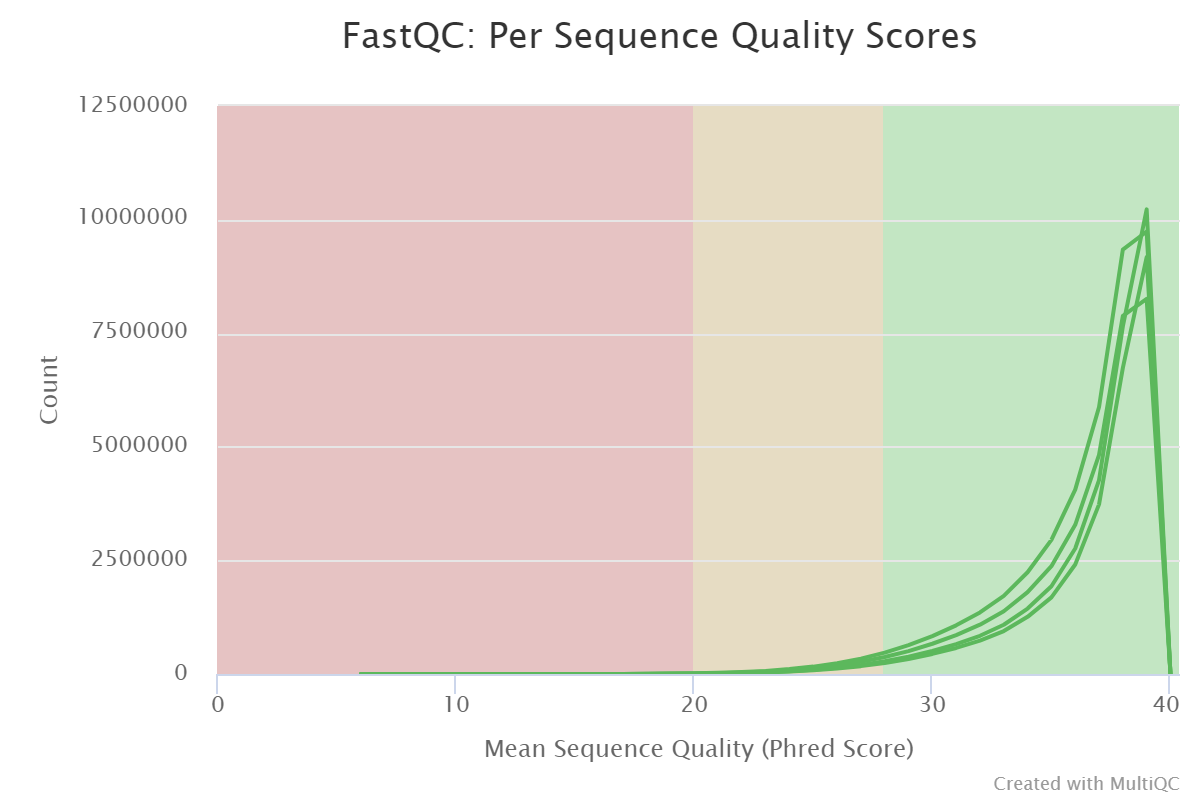
\includegraphics[width=1\textwidth]{fastqc_per_sequence_quality_scores_plot}
    \caption{The distribution of mean Phred scores across the reads.} % write about tpical pattern
    \label{fig:fastqc_per_sequence_quality_scores_plot}
\end{figure}

\newpage
Unequal read counts for each sample, as shown in \autoref{fig:fastqc_sequence_counts_plot} are expected in RNA-seq and adjusted for in the downstream pipeline. As previously stated, the presence of duplicate reads is relatively benign in RNA-seq \citep{parekh2016impact}.

\begin{figure}[!h]
    \centering
    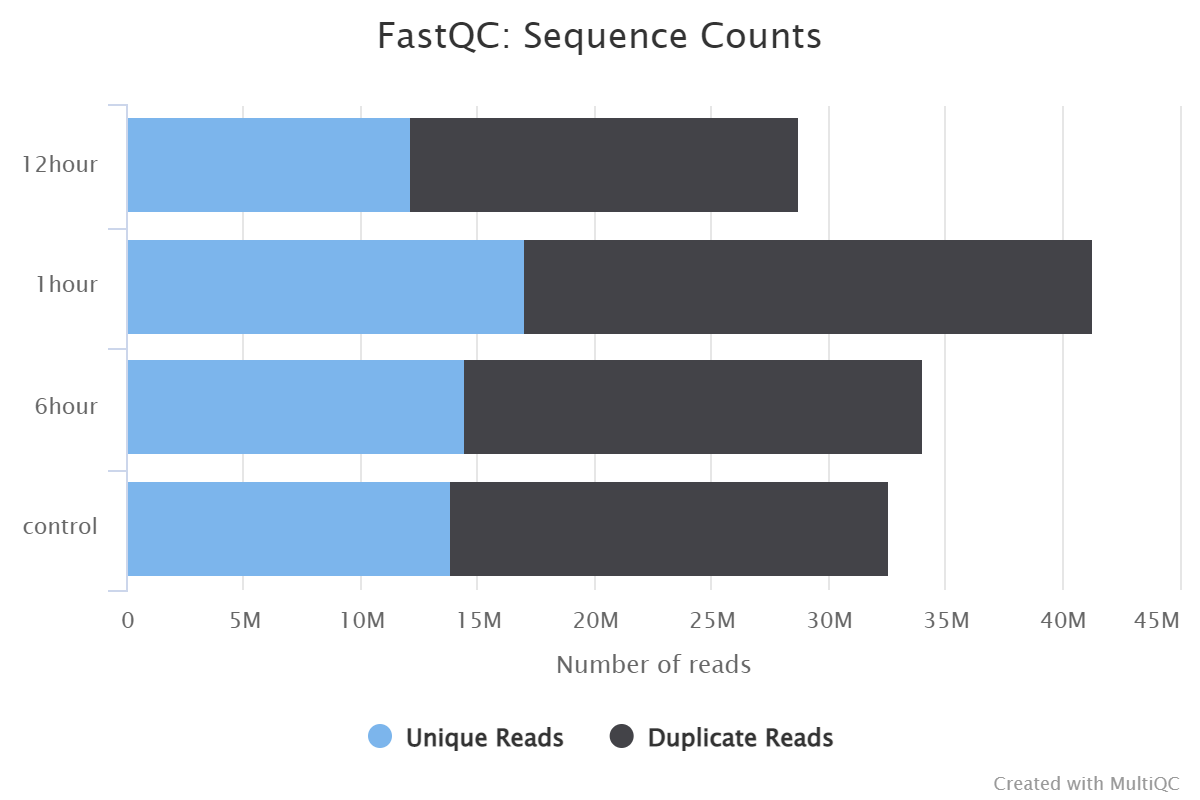
\includegraphics[width=1\textwidth]{fastqc_sequence_counts_plot}
    \caption{The number of reads for each sample, showing the proportion of duplicate reads.}
    \label{fig:fastqc_sequence_counts_plot}
\end{figure}
\newpage

The samples in \autoref{fig:fq_screen_plot} show no sign of contamination. There is an almost 100\% successful alignment to the human genome, with some alignment to other sequences which share genetic similarities. Some degree of multi-mapping (20\%) with the human reference is present. This may be caused by regions of low-complexity or by structural variants \citep{rhoads2015pacbio}

\begin{figure}[!h]
    \centering
    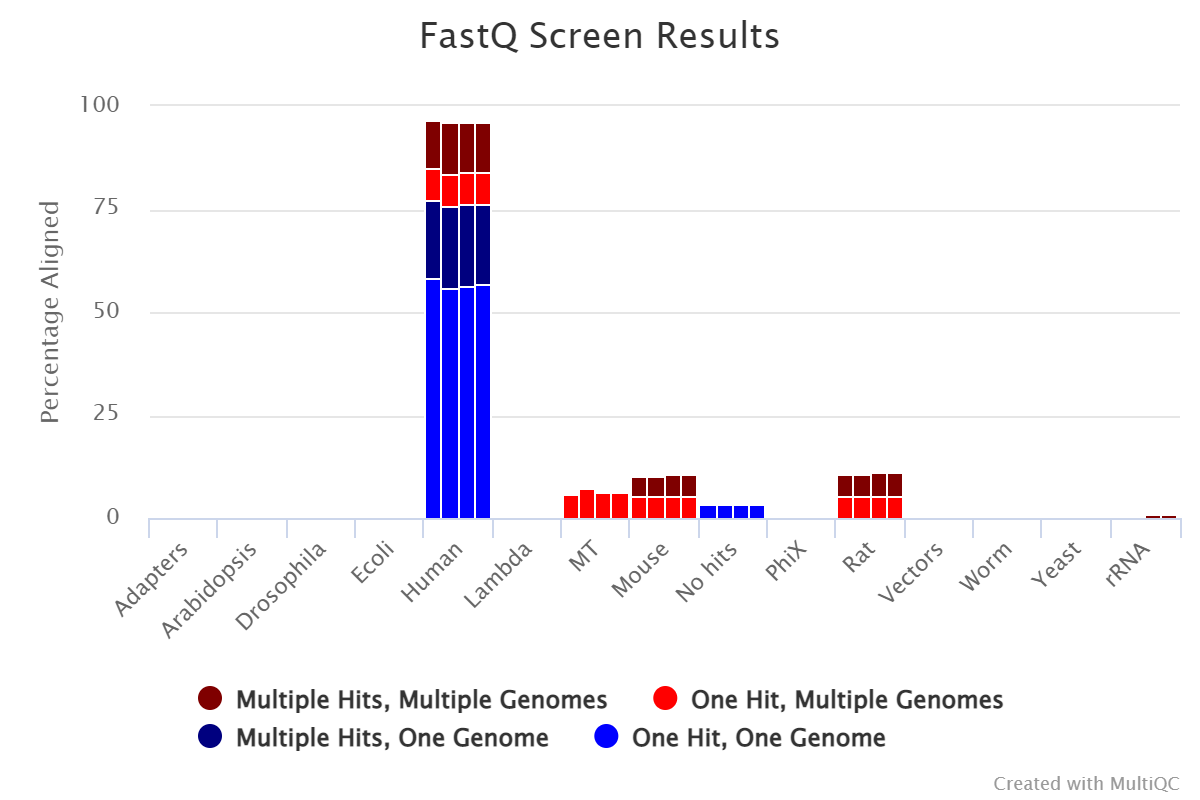
\includegraphics[width=1\textwidth]{fq_screen_plot}
    \caption{FastQ Screen plot showing the percentage of the reads aligned to which reference sequence(s).} 
    \label{fig:fq_screen_plot}
\end{figure}


\subsection{Preprocessing}
FastQC detected traces (<0.5\%) of TruSeq adapters in the FASTQ files, which is corroborated by the sequencer's manual \citep{HiSeq2000} stating that it makes use of the 'TruSeq family of reagents'. Adapter sequences were trimmed using CutAdapt (\autoref{fig:cutadapt_trimmed_sequences_plot_3}), and resultant reads shorter than 45 bp long were removed. Smaller reads lead to greater ambiguity during alignment as they have a greater probability of being multi-mapped.  The data was of good quality to begin with, so trimming had little overall effect on the reads, although the read lengths are no longer uniform.
%Between 1.3 and 1.6\% of all base-pairs were trimmed across the four samples. (why is this happening)


\begin{figure}[!h]
    \centering
    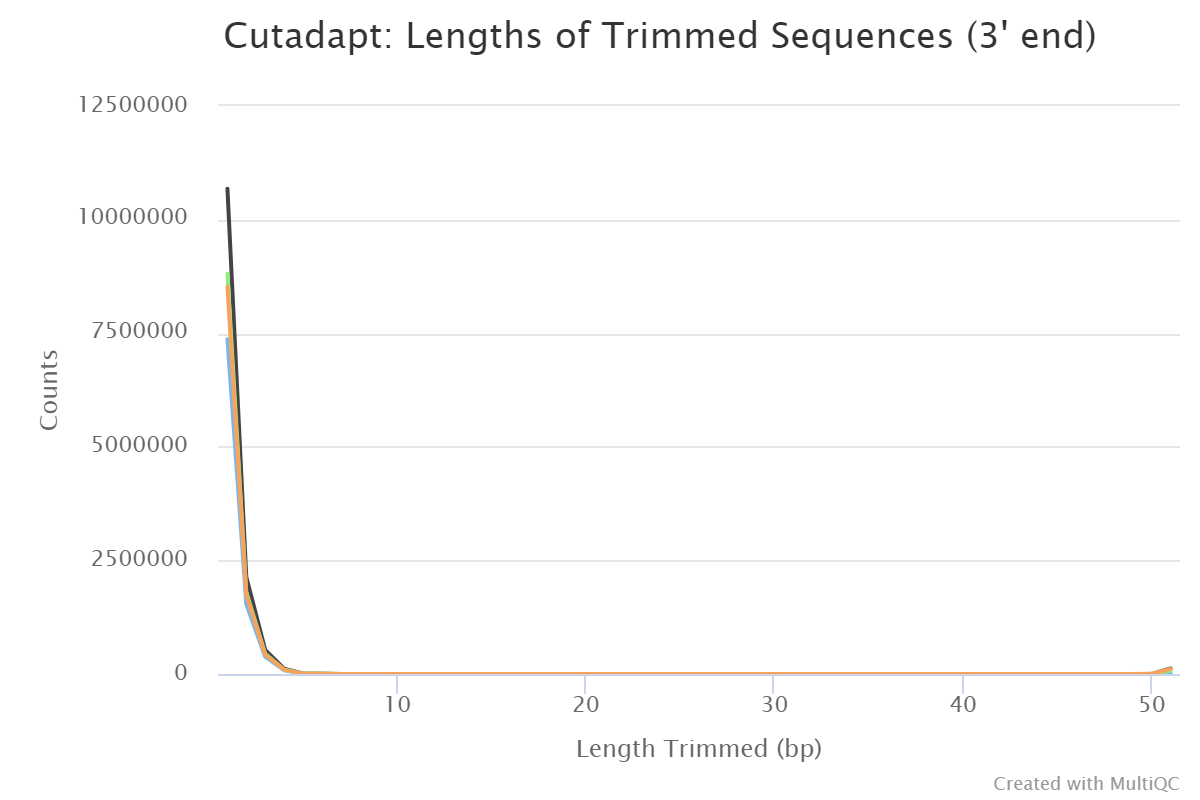
\includegraphics[width=1\textwidth]{cutadapt_trimmed_sequences_plot_3}
    \caption{The number of base-pairs trimmed per read from the 3' end.} 
    \label{fig:cutadapt_trimmed_sequences_plot_3}
\end{figure}
\newpage

MultiQC does not support Prinseq++ as of version 1.11, however its output reports are simple to interpret. They provide the number of reads filtered by \texttt{-lc\textunderscore dust} according to their DUST score (a measure of low complexity). These figures removed approximately 0.1\% of the total amount of reads for their respective sample. No reads were removed by \texttt{-ns\textunderscore max\textunderscore n} based on the number of \textit{N}'s.



\subsection{Read Alignment}
The removal of short reads and reads low in complexity has reduced ambiguity when aligning to a reference genome \citep{rhoads2015pacbio}. Nonetheless STAR experienced some degree of multimapping, shown in \autoref{fig:star_alignment_plot}. The number of loci \texttt{Nmap} a read maps to is stored in the generated BAM file as \texttt{NH:i:Nmap}. If \texttt{Nmap} exceeds a certain threshold (10 by default) it will be labelled as 'mapped to too many loci' and excluded from the final BAM file. This is the most significant filtering step so far, removing 16\% to 18\% of the total read counts. Despite the loss of this substantial chunk of our reads, the main causes \citep{rhoads2015pacbio} for multi-mapping have been mitigated where possible: 
\begin{itemize}
\item[] Low-complexity regions were filtered in the previous step using Prinseq++.
\item[] Structural variants, while frequent in cancer-derived transcriptomes, are bypassed in STAR's splice-aware algorithm \citep{Dobin2013}, allowing different parts of the same read to map to distant genomic loci (possibly to different strands or chromosomes).
\item[] Longer read lengths and paired-end reads should reduce multi-mapping, although these factors were immutable at this stage.
\end{itemize}


\begin{figure}[!h]
    \centering
    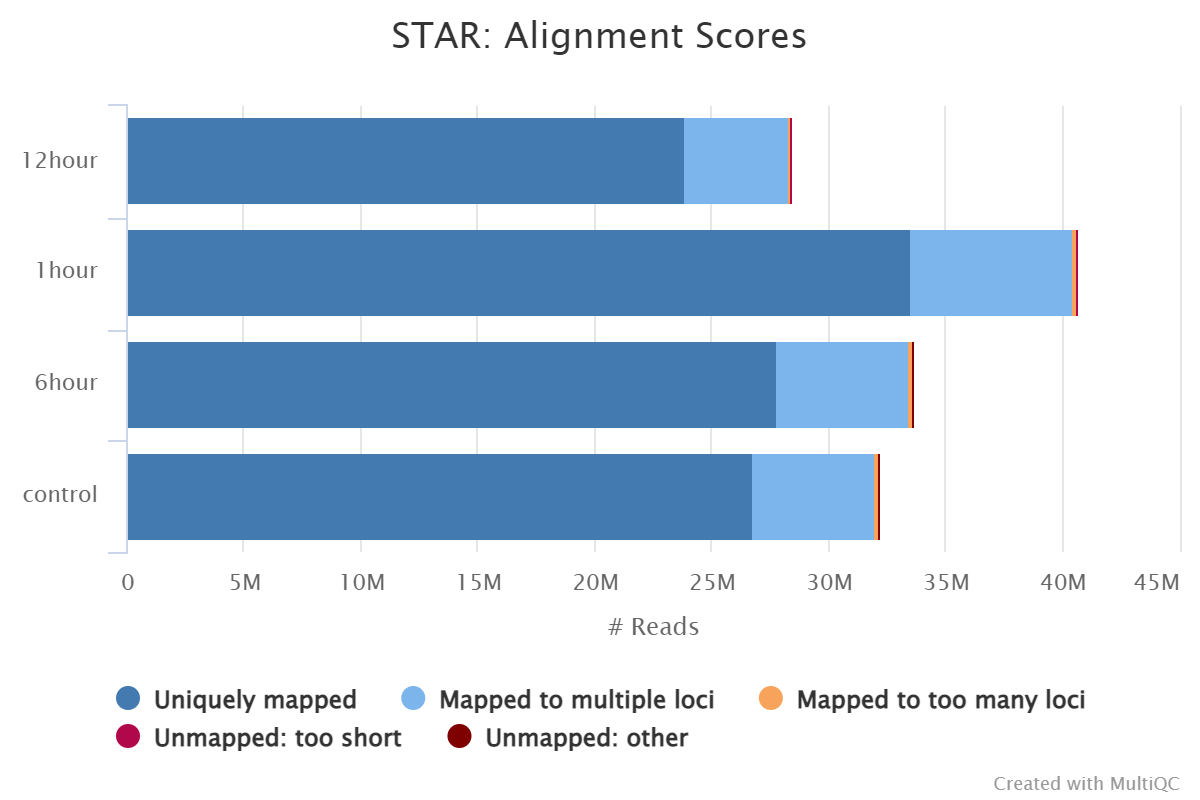
\includegraphics[width=1\textwidth]{star_alignment_plot}
    \caption{Number of uniquely mapped reads which passed all filters to the final BAM file, and the number of problematic reads which were consequently remained unaligned and were removed.} 
    \label{fig:star_alignment_plot}
\end{figure}
\newpage

%\subsection{Post-Alignment}
%At this stage tables containing information on the expected number of reads aligned to each gene are imported into R. Here we will be largely shifting our focus from the \textit{individual} reads, to \textit{collective} reads which align to each gene, i.e. to the expected read counts given in the tables produced through RSEM. The \ac{TMM} normalisation technique is performed, which adjusts the read count values per gene for confounding variables which are not biologically relevant. 

%Genes with low counts (<10) are removed as they can be considered as noise and are not expressed at any biologically meaningful level \citep{law2016rna}. These lowly expressed genes are particularly error-prone, and were shown to be highly sensitive to the \textit{in silico} methods used \citep{everaert2017benchmarking}.

\subsection{QC Summary}
The raw data in our starting FASTQ files was of good quality according to all tested metrics, resulting in Cutadapt and Prinseq++ having little effect on the read counts (\autoref{tab:read_counts}). Nonetheless a substantial portion of the reads suffered from multi-mapping and were excluded by the STAR aligner.

\begin{table}[!h]
\centering
\caption{The read counts in millions after passing through the processing tool indicated in the first column.}
\label{tab:read_counts}
\begin{tabular}{cclll}
\toprule
                                                                   & \textbf{Control} & \textbf{1 hour} & \textbf{6 hour} & \textbf{12 hour} \\ \midrule
Raw data                                       & 32.62M           & 41.30M          & 34.08M          & 28.77M           \\ 
\begin{tabular}[c]{@{}c@{}}Cutadapt\end{tabular} & 32.23M           & 40.81M          & 33.71M          & 28.54M           \\ 
\begin{tabular}[c]{@{}c@{}}Prinseq++ \end{tabular}    & 32.22M           & 40.75M          & 33.66M          & 28.50M           \\ 
\begin{tabular}[c]{@{}c@{}}STAR \end{tabular}        & 26.80M           & 33.54M          & 27.78M          & 23.89M           \\ \bottomrule
\end{tabular}
\end{table}


% The edgeR vignette suggests to use the raw counts (?) of RSEM for normalisation, as opposed to using the already normalised TPM so we went with this.
 % FPKM/RPKM are not good measures of relative abundance because the FPKM/RPKM of a transcript can change between two samples even if its relative abundance stays the same.
% https://groups.google.com/g/rsem-users/c/GRyJfEOK1BQ <- very good explanation 

%\subsection{Multiple testing Correction}
%FDR
%Benjamini Hochback 

\section{Post-Alignment Quality Control}
From this point forward we are mostly concerned with genes and the number of reads aligned to those genes in a tabular format, as opposed to individual unaligned reads. These were imported into R and converted into a \texttt{DGEList} object, \texttt{y}, consisting of multiple data-frames. The \texttt{y\$counts} dataframe initially contains the raw read count values for the four samples and a total of 60664 genes, each comprising a single row (\autoref{tab:gene_counts1}). 

In typical RNA-seq studies it is wise to search for potential batch effects and covariates, however with just a single replicate per condition it is impossible to distinguish such effects from real, biologically meaningful changes.

\begin{table}[h]
\centering
\caption{The first five out of a total 60664 rows of \texttt{y\$counts}. Notice the first two genes with low read counts which will be subsequently filtered }
\label{tab:gene_counts1}
\begin{tabular}{llllllll}
\toprule
\textbf{Genes}           & \textbf{1hr}     & \textbf{12hr}    & \textbf{6hr}     & \textbf{0hr}      \\ \midrule
ENSG00000000003 & 2       & 0       & 1       & 2        \\
ENSG00000000005 & 1       & 0       & 2       & 0        \\
ENSG00000000419 & 2491.7  & 1694.74 & 1703.4  & 1598.21  \\
ENSG00000000457 & 634.37  & 432.45  & 540.83  & 424.32   \\
ENSG00000000460 & 1176.63 & 1121.55 & 1415.17 & 1041.77  \\
...             & ...     & ...     & ...     & ... \\  \bottomrule
\end{tabular}
\end{table}

Of these 60664 genes, 43559 did not meet the minimum requirement of having at least 10 read counts for at least one sample, making them indistinguishable from noise and subsequently filtered. These counts were \ac{TMM} normalised, which did not affect the number of genes, but adjusted  read counts for between-sample differences \citep{robinson2010scaling}. The filtered and normalised data is represented holistically in \autoref{fig:boxplot_filtered}.


\begin{figure}[!h]
    \centering
    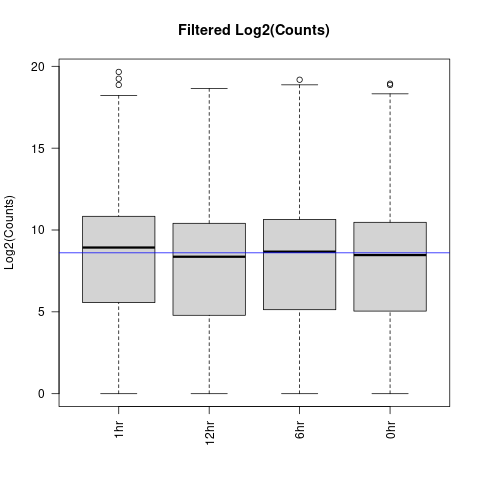
\includegraphics[width=10cm]{boxplot_filtered}
    \caption{Distribution of log$_2$-transformed counts per sample, including the control represented as '0hr'. The blue line bisecting the graph signifies the global median across all samples.} 
    \label{fig:boxplot_filtered}
\end{figure}
\clearpage

\section{Differential Gene Expression Analysis}
% Methods which compare values against a mean (e.g. Z-scores and MD-plots) are not particularly useful since we want to compare values against the control and not against the other samples
Using edgeR's classic approach \texttt{exactTest}, we compared the three treated samples (1hr, 6hr, 12hr) against the control which acted as a baseline. This generated a data frame with Ensembl gene IDs as row names, together with their respective \ac{logFC}, read counts per million, raw \textit{p}-value and \ac{FDR}. Here, the \ac{logFC} represents the \textit{magnitude} of the differential expression while the \ac{FDR} represents the \textit{significance} of the difference in expression. 

The \ac{FDR} is a form of an adjusted \textit{p}-value, applied to counteract the multiple comparisons problem arising from the hundreds of generated \textit{p}-values. This adjustment is common to RNA-seq analyses, although there is some disagreement in the literature whether it should be performed \citep{rothman1990no, streiner2011correction}, and to exercise caution when dealing with \textit{p}-values in general \citep{gardner1986confidence, greenland2016statistical, vidgen2016p}. In this study we followed the recommended edgeR procedure, using \ac{FDR}s in conjunction with the Benjamini-Hochberg controlling method \citep{benjamini1995controlling}. These values represent the probability of a type I error (i.e. a false positive result) for that specific gene. % fix this

% watch https://www.youtube.com/watch?v=K8LQSvtjcEo&ab_channel=StatQuestwithJoshStarmer

Threshold values of 1.5 for the \ac{logFC} and 0.05 for the \ac{FDR} were applied to define the truly differentially expressed genes in the data frame. With no possible objective justification of the appropriate thresholds, the choice was largely arbitrary. A \textit{p}-value cut-off of 0.05 (here, the \ac{FDR} acting as an adjusted \textit{p}-value) is a \textit{de facto} standard, popularised by Sir Ronald Fisher who stated it was "convenient to take this point as a limit in judging whether a deviation is to be considered significant or not" \citep{fisher1925statistical}. A standard \ac{logFC} cut-off does not exist, with similar studies using thresholds of anywhere between 0.5 and 2 \citep{zhao2018many, cardoso2019gene, handschuh2018gene}. One must bear in mind that this is a log$_2$ scale, and that negative values indicate a decrease in transcripts, e.g. a \ac{logFC} of -1.5 is equivalent to a third of the number of transcripts relative to the control. Absolute values are used in \ac{logFC}-based filtering to target both up- and down-regulation.

% If the phenolic treatment is successful in inducing differentiation, we should expect a divergence from a typically \ac{AML} transcriptome. The literature \citep{santos2000expression, mark2017transcriptomes} suggests that the cells will begin to exhibit monocytic or granulocytic characteristics, followed by apoptosis. This progression should be reflected in the activated JAK-STAT signaling pathway and the NF-$\kappa\beta$ pathways \citep{matikainen1997retinoic, gianni1997stat1, cohen2005jak, ren2013resveratrol, iwata2016parp9}. 



\subsection{Data Exploration}

A set of \ac{DEG}s was generated for each of the three time points, with considerable overlap between them represented as a Venn diagram in \autoref{fig:venn}. The 1hr sample shows a high proportion of uniquely expressed genes, and a higher overall number of \ac{DEG}s (\autoref{DEG_counts_barchart}). This is similarly reflected in the PCA plot, \autoref{fig:PCA_logFCs}, which shows the 1hr time point as an outlier, while the 6hr and 12hr points cluster closely. One potential hypothesis to explain this irregular spread of data is that the cells at the 1hr timepoint were in the process of differentiation and apoptosis, while the cells at 6hr and 12hr had reached a stable equilibrium, after the phenol-prone cells have died off.


\begin{figure}[!h]
    \centering
    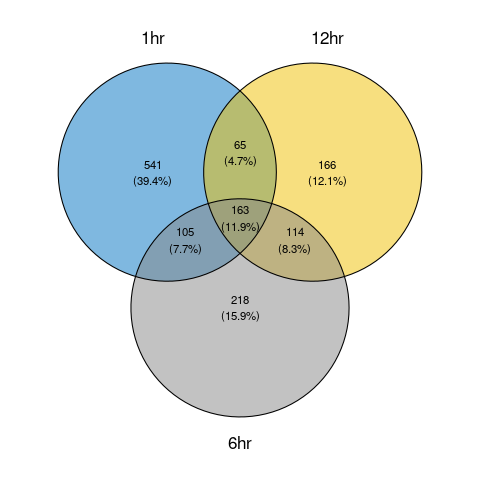
\includegraphics[width=9cm]{venn}
    \caption{Percentages of shared and unique \ac{DEG}s.} 
    \label{fig:venn}
\end{figure}

\begin{figure}[!h]
    \centering
    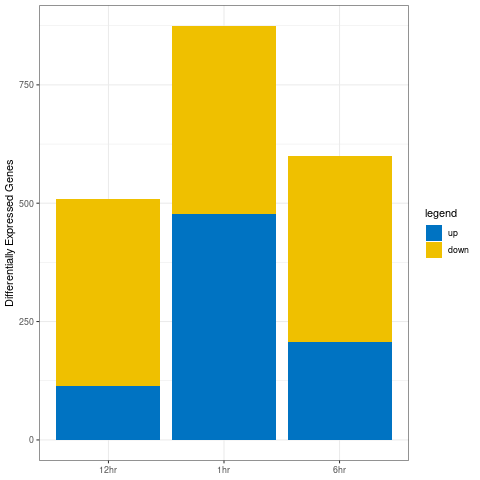
\includegraphics[width=10cm]{DEG_counts_barchart}
    \caption{Number of up- and down-regulated genes per experimental time-point.} 
    \label{fig:DEG_counts_barchart}
\end{figure}

\begin{figure}[!h]
    \centering
    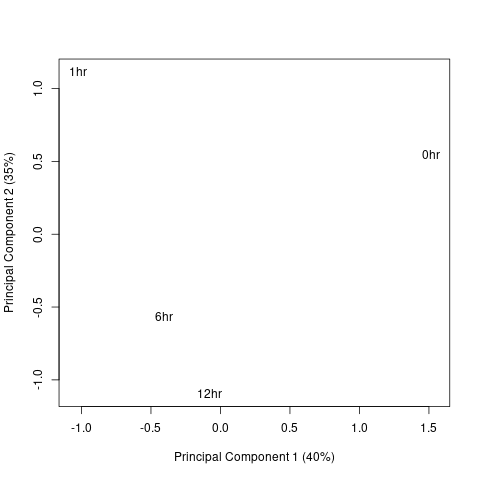
\includegraphics[width=8cm]{PCA_logFCs}
    \caption{PCA plot based on normalised counts.}
    \label{fig:PCA_logFCs}
\end{figure}
\clearpage
% Scree plot

% Bar chart of up/down for each time point

% Volcano plot
% Useful for volcano plots i think: https://huygens.science.uva.nl/VolcaNoseR/
% This too https://rdrr.io/bioc/vidger/man/vsVolcano.html


\subsection{Evaluation of Results}

We have cross-checked our resultant lists of \ac{DEG}s against a list of human housekeeping genes. These are essential to the biological function of the cell and should not change in expression levels, although exceptions to the rule exist \citep{khimani2005housekeeping}. Out of the 2833 housekeeping genes in the HRT Atlas \citep{hounkpe2021hrt}, one was found to be overly expressed in our results: ENSG00000105612. It codes for the DNase enzyme \textit{DNASE2} which plays a major role in apoptosis during foetal development \citep{yasuda1998structure}. 


\subsection{Biological Relevance of the Top DEGs}
The top 10 genes sorted by \ac{FDR}s from each of the three time points were selected for further biological investigation. The three lists were combined with considerable overlap into a single list of 17 genes, which are all protein-coding and have \ac{FDR}s of under 0.001 making them suitable candidates for further biological investigation. The \ac{FDR} was chosen for the sorting metric rather than the \ac{logFC} as it was deemed as a better indicator of biological relevance. The significance of the \ac{logFC} is tied to the role of the specific protein, i.e. a \ac{logFC} of 1.5 in a molecule with a cascading effect in a pathway may have a larger overall biological effect than a \ac{logFC} of 3 in a relatively benign molecule. The degree of up- or down-regulation of the 17 genes per time-point is shown in \autoref{heatmap_some}.

Comparing these results to the supplementary material provided by \cite{gatt2021tyrosol}, a study with particularly similar experimental design and goals, we find an overlap of 14 genes regulated the same direction. UTP14C, EGR3 and JAML were not found to be differentially expressed in \cite{gatt2021tyrosol}, while FOSB was found to be regulated but in the opposite direction.


\begin{figure}[!h]
    \centering
    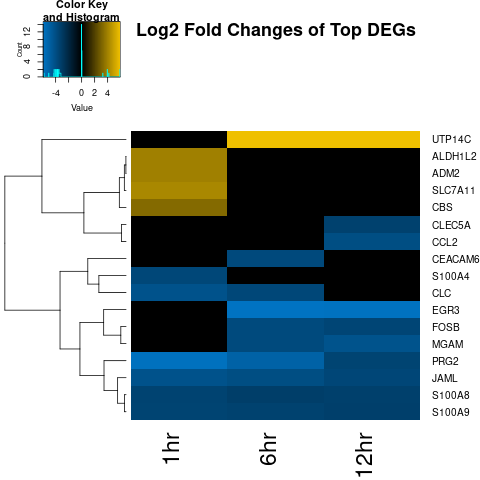
\includegraphics[width=8cm]{heatmap_some}
    \caption{The log$_2$ fold changes of the top differentially expressed genes sorted by their FDRs. The genes were originally in an ENSMBL transcript format but were translated to their gene symbol format.} 
    \label{fig:heatmap_some}
\end{figure}

% Table with FDRs and logFCs in appendix?
% write which were found in other studies


% List of DEGs from tyrosol study:  https://www.mdpi.com/2076-3417/11/21/10199
% Do the pathways make sense
% ENSG00000105612 housekeeping gene was found to be differentially expressed

% https://www.biostars.org/p/9510180/ reply says that even though a gene is downregulated, it might be suppressing other genes in the pathway which makes the other genes indirectly upregulated. Keep stuff like this in mind when interpreting gene expression.

\subsection{KEGG Pathway Visualisation}
Key KEGG pathways associated with the differentiation of \ac{AML} cells were visualised using Pathview, with \ac{DEG}s highlighted according to the direction of their regulation.



\subsection{Gene Set Enrichment Analysis}
Feeding genes in their Entrez format, and their \ac{logFC} values into the \texttt{gage} function, we have identified the significantly enriched gene sets in the form of \ac{GO} terms and \ac{KEGG} pathways. Apart from the aforementioned issue with a lack of replicates, these analyses come with a number of additional caveats, some inherent and others specific to this study:

\begin{itemize}
\item The BioStar handbook \citep{albert2020biostar} states that \ac{GO} analyses is that the results are moderately specific to the method used (this may seemingly be extended to include \ac{KEGG} pathways), with no existing objective method to validate the quality.
\item  Overlap between gene sets is possible, which may lead to some unexpectedly enriched sets. 
\item  GAGE reads genes as Entrez IDs, but our data was in the Ensembl format. Conversion was possible but imperfect since the conventions have slightly different definitions for each gene.
\item Gene sets are treated as separate entities, instead of as a part of an immensely complex and inter-connected biological system.
\end{itemize}

 %maybe find a better source for this
We have chosen a lenient FDR \textit{q}-score cut-off of 0.5, and suggest that these results be interpreted with caution. For comparison, the default GAGE cutoff was set at 0.1. \autoref{tab:gage} shows the concatenated results of the GAGE outputs for \ac{KEGG} pathways and \ac{GO} terms.


\begin{table}
\centering
\caption{Significantly enriched KEGG pathways and GO terms using a \textit{q}-value cut-off of 0.5. The \textit{Stat} column represents the generated GAGE statistic which indicates the magnitude and direction of the differential expression, analogous to the fold change in regular differentially expressed genes.}
\label{tab:gage}
\begin{tabular}{lllllll}
 \toprule
     \textbf{Gene Set} & \textbf{Term}                          & \textbf{Time} & \textbf{Stat}   & \textbf{\textit{p}-value} & \textbf{\textit{q}-value} & \textbf{\textit{N}}   \\ \midrule
            \textbf{KEGG}   \\ \midrule
hsa04145~ & phagosome                     & 1hr  & -1.963 & 0.035   & 0.039   & 10  \\
          &                               &      &        &         &         &     \\ \hline
hsa04380~ & osteoclast differentiation    & 1hr  & -1.864 & 0.039   & 0.039   & 12  \\
          &                               &      &        &         &         &     \\ \hline
hsa04380~ & osteoclast differentiation    & 6hr  & -1.882 & 0.039   & 0.039   & 13  \\
          &                               &      &        &         &         &     \\ \hline
hsa04620~ & toll-like receptor signaling~ & 12hr & -1.565 & 0.068   & 0.167   & 10  \\
          & pathway                       &      &        &         &         &     \\ \hline
hsa04145~ & phagosome                     & 12hr & -1.441 & 0.084   & 0.167   & 10  \\
          &                               &      &        &         &         &     \\ \hline
hsa04380~ & osteoclast differentiation    & 12hr & -1.136 & 0.135   & 0.180   & 12  \\
          &                               &      &        &         &         &     \\ \hline
hsa04062~ & chemokine signaling~          & 12hr & -0.454 & 0.327   & 0.327   & 11  \\
          & pathway                       &      &        &         &         &    \\ \midrule

            \textbf{GO term}   \\ \midrule
GO:0002376  & immune system process                  & 12hr & -1.998 & 0.024   & 0.408   & 67  \\
            &                                        &      &        &         &         &     \\ \hline
GO:0002376  & immune system process                  & 6hr  & -3.258 & 0.001   & 0.013   & 54  \\
            &                                        &      &        &         &         &     \\ \hline
GO:0006323~ & DNA packaging                          & 1hr  & 1.984  & 0.038   & 0.441   & 10  \\
            &                                        &      &        &         &         &     \\ \hline
GO:0006333  & ~chromatin assembly or~                & 1hr  & 1.984  & 0.038   & 0.441   & 10  \\
            & disassembly                            &      &        &         &         &     \\ \hline
GO:0006325~ & establishment, maintenance~       & 1hr  & 1.649  & 0.058   & 0.448   & 13  \\
            & of chromatin architecture                 &      &        &         &         &     \\ \hline
GO:0001775~ & cell activation                        & 1hr  & 1.181  & 0.125   & 0.472   & 13  \\
            &                                        &      &        &         &         &     \\ \hline
GO:0006520~ & amino acid metabolic            & 1hr  & 1.172  & 0.128   & 0.472   & 12  \\
            &     process                                   &      &        &         &         &     \\ \hline
GO:0006139  & ~nucleic acid metabolic ~ & 1hr  & 1.103  & 0.137   & 0.472   & 45  \\
            &    process   &      &        &         &         &     \\ \hline
GO:0006355  & ~regulation of transcription,~         & 1hr  & 1.075  & 0.144   & 0.472   & 27  \\
            & DNA-dependent                          &      &        &         &         &     \\ \hline
GO:0002376  & immune system process                  & 1hr  & -2.156 & 0.016   & 0.379   & 64  \\
            &                                        &      &        &         &         &    \\ \bottomrule
\end{tabular}
\end{table}

These gene set level results are not reflected in the literature \citep{matikainen1997retinoic, gianni1997stat1, cohen2005jak, ren2013resveratrol, iwata2016parp9}, which has repeatedly shown that the JAK-STAT signaling pathway and the NF-$\kappa\beta$ pathway play an essential role in differentiation of \ac{AML}, and are activated by differentiation agents. \cite{gatt2021tyrosol} found the \textit{Myeloid differentiation} \ac{GO} term (\ac{GO}:0030099) to be especially significant at an \ac{FDR} of 0.0001. Combined with the high \textit{q}-scores and the aforementioned caveats, interpretation of these results is difficult and only give a weak indication of the effectiveness of the treatment. 

Nevertheless, it is clear that overall the gene sets in \cite{tab:gage} somehow link to morphologically changing myeloid cells, particularly the \ac{GO} terms for the 1hr sample. The up-regulation of GO:0001775 is particularly indicative, which is defined\footnote{\url{https://gowiki.tamu.edu/wiki/index.php/Category:GO:0001775_!_cell_activation} (Last accessed 29/06/22)} as "a change in the morphology or behaviour of a cell resulting from exposure to an activating factor such as a cellular or soluble ligand."


%Pathview results

% good resource: https://ressources.france-bioinformatique.fr/sites/default/files/4%20-%20FGSA_Roscoff.pdf
% Resulting enriched pathways -> statistical probability rather than a biological certainty


\section{Summary}
\enlargethispage{\baselineskip} % so you do not get a single line in another page

    %\chapter{Conclusions}

This section should have a summary of the whole project.  The original aims and objective and whether these have been met should be discussed. It should include a section with a critique and a list of limitations of your proposed solutions.  Future work should be described, and this should not be marginal or silly (e.g.\ add machine learning models).  It is always good to end on a positive note (i.e.\ `Final Remarks').

\section{Revisiting the Aims and Objectives}
\blindtext

\section{Critique and Limitations}
\blindtext

\section{Future Work}
\blindtext

\section{Final Remarks}
\blindtext

    %\appendix
    %     \chapter{Media Content}

If the dissertation has a DVD or pendrive attached to it, you will need a section which explains what is on the media (structure, files, data, etc.).  This could be a table with filename and description.

\blindtext[5]
     
    %     \chapter{Installation Instructions}
\blindtext[10]



\pagestyle{umpageback}
{\backmatter
    % Bibliography
    \if@openright\cleardoublepage\else\clearpage\fi

    \bibliographystyle{um-plainnat} %% specific plainnat does not show url for articles
    % Use something like https://flamingtempura.github.io/bibtex-tidy/ to clean all your bibtex entries
    { 	\scriptsize\bibliography{intro/introduction_biblio,lit_review/background_and_lit_overview_biblio, method/materials_and_methods_biblio, results/results_and_discussion_biblio, evaluation/evaluation_biblio, conclusion/conclusions_biblio}}
	\printindex
}

\end{document}
% There is a hard limit of 32k words
% Last check was on 19/06/22 and we re on ~21k words

%%% The End %%%
